\chapter{METHODOLOGY AND RESULTS}
\label{ch:methodology-results}

% Overview of chapter
\section{Overview}

% About the hypotheses and objectives
% About the user selection criteria
In this chapter, we briefly revisit the objectives of this work to formulate the hypotheses and methodology for our experiment. We establish the selection criteria for the users in our experiment, which enforce restrictions to provide a more controllable environment given societarial restrictions inherent to the time at which this work was developed.

% About the classification of the user base
% About the methodology of the experiment
We specify the classification method used in this experiment, which was employed to compare the effects of our DDA system to different types of users, in comparison to the traditional fixed difficulty presets commonly seen in commercial games. In sequence, we explain the methodology used in our experiment, specifying the division of user groups, describing the metrics used to compare such groups, providing a brief description of the steps performed by users in the experiment, and providing details on a survey used to assess user perceptions after performing the experiment.

% About the analysis of results 
Finally, we report and analyze the results of our experiment, performing a comparison of the performance of user groups when using DDA systems or fixed difficulty. We perform a more granular comparison by separating  the data for each group based on our initial user classification, and assess the effects of DDA systems on each player profile: \emph{beginners}, \emph{intermediates} and \emph{veterans}. We also compare the performance of players to their own assessment of the difficulty of our game, and correlate their perception with our performance analysis.

% ======================================================================
% ======================================================================
% =================================================================

\section{Hypotheses and Objectives}
\label{sec:hypotheses-and-objectives}

% Main Objectives
% ===================
%       - Verify if dynamic adjustments create an increase in the performance over the play session for beginner & intermediate players
%       - Verify if dynamic adjustments keep a fair challenge, without overt increases in performance for advanced players
As a first objective when performing this experiment, we wish to verify if dynamic adjustments can create a relevant increase in player performance in the first or second playthrough for players that are inexperienced with \emph{Souls-like} games. We attempt to understand if players that experience dynamic difficulty at their first playthrough can achieve a better understanding of game mechanics on their second playthrough.

We also wish to understand if dynamic difficulty can maintain a fair level of challenge to veterans or experienced players on a second playthrough. To do this, we wish to evaluate the difference in performance between fixed and dynamic difficulty on a second playthrough where players have likely increased their performance when using game mechanics. Based on these objectives, we formulate the following hypotheses:

% * Hypotheses
% * ====================================
% Hypothesis 1: Dynamic can alleviate the learning curve for beginners
% Hypothesis 2: Dynamic is less frustrating than fixed for beginners
% Hypothesis 3: Dynamic can keep a better challenge on 2nd+ playthrough
% Hypothesis 4: Dynamic is not overtly easy to veterans
\begin{itemize}
    \item{Hypothesis 1: Dynamic difficulty can alleviate the steep learning curve of challenging games for inexperienced players;}
    \item{Hypothesis 2: Dynamic difficulty can provide a better suited level of challenge on the second or subsequent playthroughs.}
\end{itemize}

The hypotheses defined have the intent of comparing DDA systems to fixed difficulty on two different aspects: the ability for players to learn and become used to \emph{Souls-like} game mechanics in a first playthrough, and the ability for the game to provide a sufficient level of challenge to players which have become accustomed to and proficient at the game at a second or subsequent playthrough.

% Validation of Hypothesis 1
% =========================

% Most common causes of failure are discovery
As discussed in chapter \ref{ch:analysis-object-study}, the most prevalent causes of failure in first playthroughs of \emph{Souls-like} games include becoming used to the game's input and its resulting actions, understanding the principles of the most relevant game mechanics, and memorizing patterns of enemies or level layouts. In a second playthrough, players will generally have achieved a consolidated understanding of which elements provide the most significant challenge, and how to use the game's mechanics in a way that maximizes their chances of success.

% We wish to validate that 
Therefore, failure is often part of the process of learning in a first playthrough. Presenting the player with a slight difficulty spike at a specific point in the game could be a tool to accelerate the process of learning a specific game mechanic, given that the level of challenge is not overtly contrasted to the player's skill. Thus, we wish to validate our hypothesis that the performance of players which experience Dynamic Difficulty first is higher than those which experience fixed difficulty first, as they become used to the game's mechanics and challenges.

% Validation of hypothesis 1
To perform the validation of Hypothesis 1, we divide the users in our experiment in two groups: users which experience Fixed Difficulty first (Group A), and users which experience Dynamic Difficulty systems first (Group B). After performing such division, we must evaluate the performance of each group according to level progression in their first playthrough, by gathering multiple performance statistics for each level. To validate the hypothesis, we must validate that the average performance of Group B is higher than the performance of Group A. Therefore, the \emph{null hypothesis} of Hypothesis 1 is that the average performance of Group A is the same or higher than the performance of Group B.

% Validation of Hypothesis 2
% =========================

In a second playthrough, players will have experienced and become used to most or all relevant game mechanics or difficulty factors. In consequence, most players will be able to devise one or multiple plans of action against challenging elements ahead of time, and attempt to execute such plans. 

Therefore, the most prevalent cause of failure in a second playthrough with fixed difficulty is a failure of execution, where the player either performs their input incorrectly, or their plan of action does not optimally address the issues inherent to a specific challenge. As a consequence, players will generally present a much better performance in a second playthrough in fixed difficulty systems.

However, when the advent of dynamic difficulty is employed, the game is able to present new challenges and situations, and even increase the complexity at which a game mechanic needs to be executed by the player. Therefore, even though players are used to most or all game mechanics in a second playthrough, their performance can stay at the same or a lower level than that of the first playthrough. Therefore, we wish to evaluate the performance of players in a second playthrough, which occurs in the second part of the experiment.

To validate Hypothesis 2, we wish to verify that the average performance of Group A (which starts with fixed difficulty) is the same or lower than the average performance of Group B (which starts with dynamic difficulty). Therefore, the \emph{null hypothesis} of Hypothesis 2 is that the average performance of Group B is significantly higher than that of Group A in a second playthrough.

% =================================================================

% * Scenarios
% * ====================================

% * Variables
% * ====================================

% =================================================================
% =================================================================
% =================================================================

\section{User Selection Criteria}
\label{sec:user-selection-criteria}
% * User selection criteria
% * ====================================

\sepfootnotecontent{fn:bloodborne}{Bloodborne (FromSoftware, 2015). Video Game. Available on PlayStation 4.}
\sepfootnotecontent{fn:sekiro}{Sekiro: Shadows Die Twice (FromSoftware, 2019). Video Game. Available on PlayStation 4, Xbox One, Microsoft Windows, Google Stadia.}
\sepfootnotecontent{fn:steam}{\emph{Steam} is an online storefront and a digital service for video game distribution, developed by \emph{Valve}. Features provided by Steam include digital rights management, social networking, cloud-based game saving systems, automatic game updating and streaming.}

The methodology used for our experiment involves the deployment and use of our application in environments where the users are comfortable playing, without in-person monitoring by the experiment observers. For the analysis of user performance and results, we remotely collect data through telemetry, and compare data sets based on user classification and use the results of our player perception surveys as a reference. We employed restricted selection criteria for our user base to ensure similar characteristics on how the application is used.

The selection of users for our experiment was guided by a small set of profile characteristics and hardware requirements. This was required to mitigate the impact of external and unmanageable factors such as preferences, age, platform or input devices to the performance of users. Users were invited for the experiment through multiple Brazilian online gaming communities using the \emph{Discord} application. The targeted groups included communities with players of all skill levels, with the shared common interest of discussing  \emph{Souls-like} games, such as \emph{Dark Souls}, \emph{Bloodborne}\sepfootnote{fn:bloodborne} and \emph{Sekiro}\sepfootnote{fn:sekiro}. We define in the list below the profile-based criteria for user selection performed in our experiment:
% Player profile
% ===================
%   - Age: 18-23
%   - Plays Console or PC video games
%   - Prefers the use of joystick controllers
%   - Has a Steam account
\begin{itemize}
    \item{\emph{Age:} between 18 and 23 years old;}
    \item{\emph{Preffered gaming platforms:} Video Game Consoles or Desktop PC;}
    \item{\emph{Preffered input methods:} dual-analog joysticks;}
    \item{\emph{Additional requirements:} has a Steam\sepfootnote{fn:steam} account.}
\end{itemize}

% \subsection{Hardware Requirements}
% Hardware requirements
% ===================
We also require users to possess hardware that satisfies the proper execution of our application under a target framerate of 60 frames per second, to ensure that player performance is not affected by low graphical performance, stuttering or input lag. In the list below we specify the hardware requirements to properly execute our application under our specified hardware performance targets:
% Hardware Requirements \\
% 64 bit processor and Operating System \\
% Processor: Intel Core i5-2300 2.8GHz+ or AMD FX-6300 3.5GHz+ \\
% Graphics: NVIDIA GeForce GTX 460 or AMD Radeon 5000 series+ \\
% DirectX: Version 11+ \\
% Operating System: Windows 7 64bit, Service Pack 1+ \\
% Memory: 6GB+ RAM \\
% Available Storage: 4GB+ available on HDD or SSD \\
% 16:9 or 16:10 monitor between 19" and 24" and at least 1280x720 native resolution \\
\begin{itemize}
    \item{\emph{System Architecture:} 64 bit processor and Operating System;}
    \item{\emph{Processor:} Intel Core i5-2300 2.8GHz+ or AMD FX-6300 3.5GHz+;}
    \item{\emph{Graphics:} NVIDIA GeForce GTX 460 or AMD Radeon 5000 series+;}
    \item{\emph{DirectX:} Version 11+;}
    \item{\emph{Operating System:} Windows 7 64bit, Service Pack 1+}
    \item{\emph{Memory:} 6GB+ RAM}
    \item{\emph{Available Storage:} 4GB+ available on HDD or SSD}
    \item{\emph{Display:} 16:9 or 16:10 monitor sized between 19" and 32" and at least 1280x720 native resolution.}
\end{itemize}

% \subsection{Required Peripherals \& Input Methods}
We also require that players use similar input interface methods, to ensure that the accuracy of performed actions such as character movement, camera movement, dodging or blocking are not affected by restrictions on input devices, such as a computer keyboard not being able to represent directional movement with the same level of freedom as a dual-analog joystick. In the following list we specify the characteristics used to define the input interfaces required to be used by players in our experiment:  
% Required Peripherals & Input
% ===================
% Required peripherals and input: \\
%  - Joystick controller:  \\
%      - Xbox Controllers: Xbox 360, Xbox One, Xbox Series X \\
%      - Playstation Controllers: DualShock 3, Dual Shock 4, Dual Sense \\
%      - Or equivalent models with at least: \\
%          - Dual analogs \\
%          - 4 face buttons \\
%          - 4 digital directional buttons \\
%          - Right and left triggers and bumpers
\begin{itemize}
    \item{\emph{Xbox Controllers:} Xbox 360, Xbox One, Xbox Series X;}
    \item{\emph{PlayStation Controllers:} DualShock 3, DualShock 4, Dual Sense;}
    \item{\emph{Equivalent Joystick Controller Models} with at least:}
    \begin{itemize}
        \item{Dual Analog axes, one at each side;}
        \item{A clickable Trigger Button at each analog axis;}
        \item{4 Face Buttons in the right side;}
        \item{4 Digital Directional Buttons in the left side;}
        \item{Right and Left Triggers and Bumpers at the top.}
    \end{itemize}
\end{itemize}

We apply some of the aforementioned criteria through a \emph{Player Classification Survey}, which is further detailed in section \ref{sec:user-base-classification}. The Player Classification survey is also used to categorize our users in skill-based classification groups, such as \emph{Beginner}, \emph{Intermediate} and \emph{Veteran} users. Information on the specific questions and metrics used in the classification survey can be seen in appendix \ref{anx:player-classification-survey}. Regarding the topics not covered in the classification survey, we applied a secondary \emph{Player Experiment Requirements Survey}, which can be seen in \ref{anx:player-experiment-requirements-survey}

% TODO add photo of how the environment for the experiment was supposed to be

% =================================================================
% =================================================================
% =================================================================

\section{Classification of the User Base}
\label{sec:user-base-classification}
% * User classification groups
% * ====================================

We define user classification groups which are used to divide our data sets based on expected levels of player skill. Such classification is necessary to evaluate the impact of difficulty and dynamic difficulty adjustments based on player expertise. Additionally, we also use such classification to evaluate the opinions of different players on the validity of our application as a sufficient representative of the core aspects of our object of study, \emph{Dark Souls}. The classification is performed based on a \emph{Player Classification Survey}, which was performed during the User Selection step of our experiment.

% Objective
% ===================
%   - Separate players in beginners, intermediate, veterans
%       - Beginners: casuals, unused to action games
%       - Intermediate: average, used to action games
%       - Veterans:  hardcore, used to action & Souls-like games

% Classification Groups
% ===================
%   - Beginners:
%       - Never played a souls-like
%       - Low experience in action games
%       - Low avg. playtime
%   - Intermediate
%       - Previously played souls-likes
%       - Never finished a souls-like
%       - Medium or high experience in action games
%       - Moderate or high avg. playtime
%   - Veterans
%       - Finished one or multiple souls-likes
%       - High experience in action games
%       - High avg. playtime

We separate the player base in our experiment in the following groups: \emph{beginners}, \emph{intermediate} and \emph{veterans}. We define general descriptions for each group to serve as a guide when defining functional and data-based metrics which can be applied to our Player Classification Survey:

\begin{itemize}
    \item{\emph{Beginners:} casual players which are unused to playing action games, or players which are initiating their first playthrough on a \emph{Souls-like} game;}
    \item{\emph{Intermediate:} recurrent players which are used to action games, and have finished or relevantly progressed through a single \emph{Souls-like} game;}
    \item{\emph{Veterans:} dedicated players which are used to the \emph{Souls-like} genre, and have finished multiple games of FromSoftware's \emph{Souls} franchise.}
\end{itemize}

% Metrics
% ===================
%   - Avg. Playtime per Week
%   - Experience in action games
%   - Completion of Souls-likes

With such descriptions, we can begin to specify each categorization in functional or data-based terminology. We use the definitions of \emph{casual} and \emph{hardcore} players from the work of  \citet{ARTICLE_CasualsHardcoreDefinition} as a reference, where casual players are defined as individuals which perform the act of play \emph{casually} -- who dedicate a smaller portion of their time to play games, and usually on a more restricted set of genres.

Therefore, we define \emph{beginner} players as players with a weekly playtime between 0 and 3 hours, which are comfortable with at most three different game genres which do not include action games, and have not achieved 50\% completion on a \emph{Souls-like} game. \emph{Intermediate} players have a weekly playtime between 4 and 10 hours, are comfortable with at least three game genres which include action games, and have achieved at least 50\% completion on a single \emph{Souls-like} game. \emph{Veteran} players have a weekly playtime above 10 hours, have at least four comfortable game genres which include action games, and have completed two or more \emph{Souls-like} games.

% User base
% ===================
%   - Total number: 23
%       - Beginners: 10
%       - Intermediates: 7
%       - Veterans: 6

The total number of users which participated in ther experiment and sufficiently satisfied our selection criteria was 23, where 10 users were classified as \emph{beginners}, 7 were classified as \emph{intermediates}, and 6 were classified as \emph{veterans}. Unfortunately, we were unable to acquire an even number of intermediate candidates for a symmetrical division. As will be explained in section \ref{sec:experiment-methodology}, we divided our total user base in two groups. Table \ref{tab:user-base-sizes} specifies the definition used in our experiment for each user category, as well as the amount of users in each category which participated in our experiment.

% Event Instance
%   • Timestamp ( Time : double )
%   • Name ( String )
%   • Category ( String )
%   • Source ( ObjectId : GUID )
%   • Params[]
%       • { "name", "type", "value" }

% Table with user classifications
\begin{table}[!ht]
    \begin{center}
      \caption{Users for each user classification category in our experiment.}
      \label{tab:user-base-sizes}
      \rowcolors{2}{}{gray!25} % Alternate row colors
      \begin{tabular}{ w{l}{5em} w{r}{2em} m{25em} } % alignments and column size
        \addlinespace
        \toprule
        % Headings
        \bf Group & \bf Users  & \bf Definition \\
        \midrule
        % Data
        Beginners & 10 & Weekly playtime between 0 and 3 hours; Comfortable with at most 3 different genres different than action games; Have not achieved 50\% completion on a \emph{Souls-like} game. \\
        Intermediate & 7 & Weekly playtime between 4 and 10 hours; Comfortable with at least 3 game genres which include action games; Have achieved at least 50\% completion on a single \emph{Souls-like} game. \\
        Veterans & 6 & Weekly playtime above 10 hours; Have at least 4 comfortable game genres which include action games; Have completed two or more \emph{Souls-like} games. \\
        Total & 23 & All players in our experiment. \\
        \bottomrule
      \end{tabular}
    \end{center}
\end{table}

% =================================================================
% =================================================================
% =================================================================

\section{Experiment Methodology}
% * Experiment 2: Validation of Adaptive Solution
% * ====================================
\label{sec:experiment-methodology}

% * Methodology
% * =======================

\subsection{User Groups}

% Division of user groups
% ===================
%   - Group A: Fixed first, adaptive second
%       - Segment 1: Fixed difficulty modes
%       - Segment 2: N-dimensional adaptive difficulty
%   - Group B: Adaptive first, fixed second
%       - Segment 1: N-dimensional adaptive difficulty
%       - Segment 2: Fixed difficulty modes

As specified in the earlier sections of this chapter, we divide our user base in two similarly sized groups to evaluate the effects of DDA systems in the learning curve for beginners and in the challenge level for proficient players:
\begin{itemize}
    \item{Group A: Fixed Difficulty in the first playthrough (Part 1), and Dynamic Difficulty in the second playthrough (Part 2);}
    \item{Group B: Dynamic Difficulty in the first playthrough (Part 1), and Fixed Difficulty in the second playthrough (Part 2).}
\end{itemize}

% Number in user groups
% ===================
%   - Group A: 12
%       - Beginners: 5
%       - Intermediates: 4
%       - Veterans: 3
%   - Group B: 11
%       - Beginners:  5
%       - Intermediates: 3
%       - Veterans: 3

We attempted to divide our user base simetrically based on each category, as a means to attempt to compare the statistics of each group with the same sample size. Each group contains the same or a similar amount of users for each classification described in section \ref{sec:user-base-classification}. As a result, \emph{Group A} consisted of a total amount of 12 users, with 5 beginners, 4 intermediates and 3 veterans. \emph{Group B} consisted of 11 users, with 5 beginners, 4 intermediates and 3 veterans. Figure \ref{fig:user-group-sizes} illustrates the division and sample size of each user group, separating each group in the classifications defined in section \ref{sec:user-base-classification}.

% Figure with consolidated user group numbers
\begin{figure}[!ht]
    \begin{center}
    \caption{Chart representing the size of each experiment group, separated by our user classification.}
        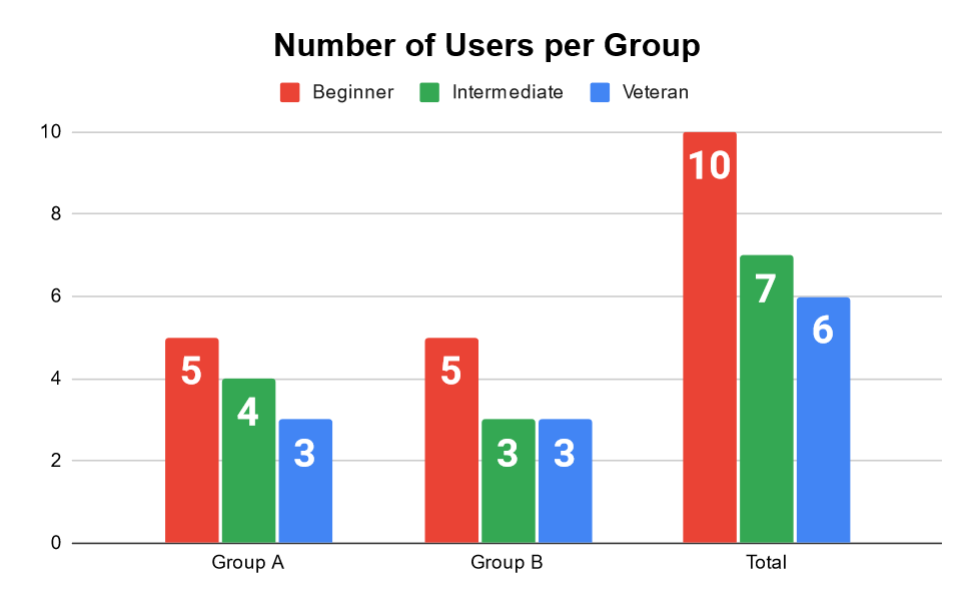
\includegraphics[width=22em]{figures/fig-user-groups.png}
        \legend{Source: Chart assembled by authors.}
        \label{fig:user-group-sizes}
    \end{center}
\end{figure}

\subsection{Experiment Flow}

% Experiment overview
% ===================
%   - Step 1: Perform player classification survey
%       - Be classified as beginner, intermediate, 
%   - Step 2: Be assigned to Group A or Group B
%   - Step 3: Play through part 1
%   - Step 4: Play through part 2
%   - Step 5: Perform player perception & comparison survey

Regarding the execution of our experiment, we defined a series of steps to be performed by users for the authors to be able to classify and divide users, and in sequence collect the performance and perception data of users:

\begin{enumerate}
    \item{User performs the Player Classification Survey;}
    \item{User is classified as a Beginner, Intermediate or Veteran;}
    \item{User is assigned to Group A or Group B;}
    \item{User plays through Part 1 of the Experiment (First Playthrough);}
    \item{User plays through Part 2 of the Experiment (Second Playthrough);}
    \item{User performs the Player Perception Survey.}
\end{enumerate}

% Figure with consolidated user group numbers
\begin{figure}[!ht]
    \begin{center}
    \caption{Diagram representing the steps performed by users in our experiment.}
        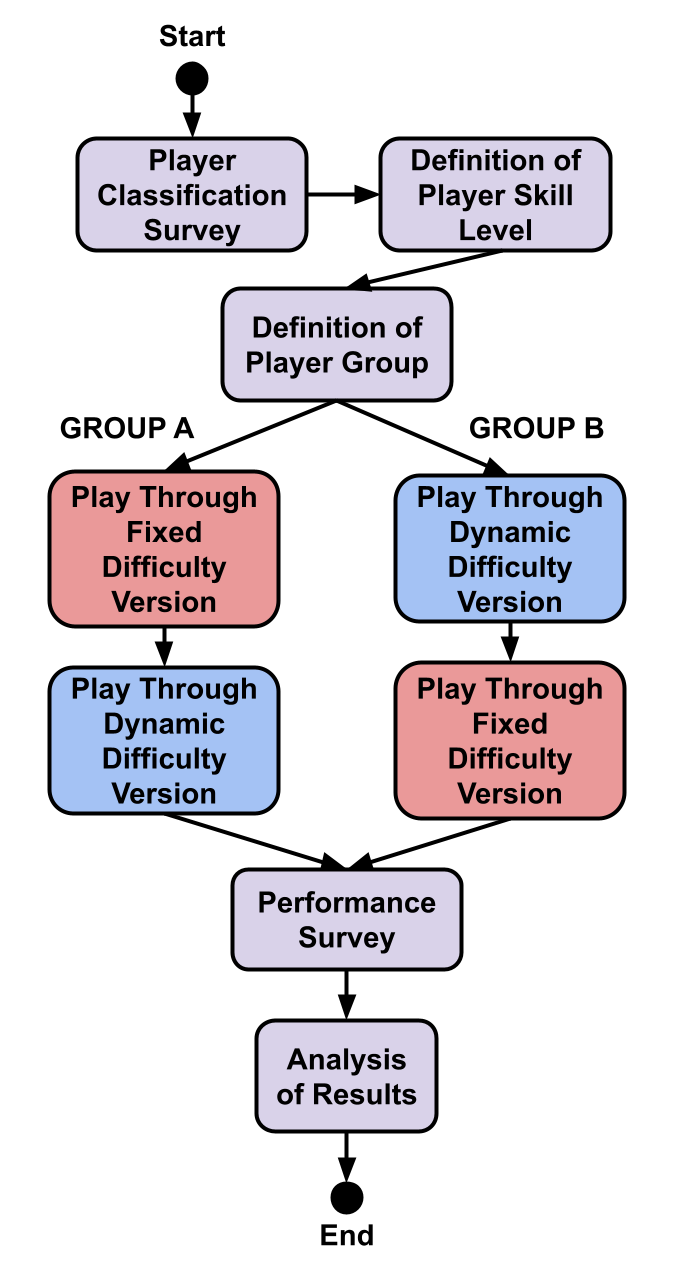
\includegraphics[width=17em]{figures/fig-experiment-flow.png}
        \legend{Source: Diagram assembled by authors.}
        \label{fig:experiment-flow}
    \end{center}
\end{figure}

Figure \ref{fig:experiment-flow} illustrates the aforementioned process in the form of a diagram. There are additional steps which were occluded due to being unrelated to the process of acquiring and evaluating data for the purpose of our experiment. For instance, between a user performing the Player Classification Survey and being classified, users also performed the Experiment Requirement Survey, as it was a necessary step to evaluate if the user hardware was performant enough to run our application.

Additionally, it is important to note that there was no automated method assign users to a classification or a group. Instead, the authors of this work manually analyzed the data and classified users based on observable clusters of data. For the definition of which users would be assigned to each group, a simple symmetrical division was performed without considering any classification-based metrics.

\subsection{Metrics}

% Explanation of used Metrics
% ===================

% Negative Metrics (lower is better)
%   - Avg. Completion Time per Level
%   - Avg. Number of Deaths Per Level
%   - Avg. Health Lost Per Encounter

% Positive Metrics (higher is better)
%   - Avg. Attack Avoidance Efficiency
%   - Avg. Attack Window Efficiency
%   - Avg. Damage Dealt Per 10s In Encounters
%   - Avg. Stamina Level In Encounters

To verify the validity of our hypotheses in each group, we gathered a subset of the metrics which are originally calculated by our application to serve as input for adjustment policies. Such metrics are selected based on their relevance in assessing the overall performance of a player, which will be evaluated in the context of the first and second playthroughs.

Furthermore, we specifically wish to evaluate performance regarding the effectiveness of players to complete game levels -- which includes traversing through environments, defeating enemies and avoiding defeat. Therefore, the metrics selected to define player performance in this experiment attempt to satisfy the efficiency and effectiveness of players when performing game mechanics which help them complete levels faster, defeat enemies faster and avoiding taking damage.

Thus, we selected the following metrics as our objects of analysis: \emph{Average Completion Time per Level}, \emph{Average Number of Deaths per Level}, \emph{Avg. Health Lost per Encounter per Level}, \emph{Average Attack Avoidance Efficiency}, \emph{Average Attack Window Efficiency}, \emph{Average Damage Dealt per 10s in Encounters} and \emph{Average Stamina Level in Encounters}. Table \ref{tab:descriptions-performance-metrics} attempts to provide a brief description of the purpose and unit of measure of each selected metric.

% Table with Descriptions for Performance Metrics used for Evaluating Player Performance
\begin{table}[!ht]
    \begin{center}
      \caption{Descriptions of the Performance Metrics used to evaluate Players.}
      \label{tab:descriptions-performance-metrics}
      \rowcolors{2}{}{gray!25} % Alternate row colors
      \begin{tabular}{ w{c}{6em} m{27em} } % alignments and column size
        \addlinespace
        \toprule
        % Headings
        \bf Metric & \bf Description  \\
        \midrule
        % Data
        \makecell[c]{Adjustment\\Targets\\Average} & Consolidated average $x$ of all \emph{ajustment target} values $v_n \in \{1, 2, 3\}$ of a player at a given level. A value of 1 in this metric would mean that all adjustment values would map to the beginner-level fixed difficulty, while a value of 3 would mean that all adjustment values would map to the veteran-level fixed difficulty. \\
        \makecell[c]{Attack\\Avoidance\\Efficiency} & The percent of attacks, with value $v \in \mathbb{R}(0, 1)$, that the player successfully avoids at a given level by \emph{dodging}, \emph{blocking} or simply moving away from the attack's area of effect. \\
        \makecell[c]{Attack\\Window\\Efficiency} & The percent of time, with value $v \in \mathbb{R}(0, 1)$, in which an enemy character is \emph{vulnerable} and the player is performing an attack. A \emph{vulnerable} enemy is in one of the following conditions: \emph{staggered}, in an \emph{animation lock} or in \emph{cooldown}. \\
        \makecell[c]{Completion\\Time} & The amount of time, with value $v \in \mathbb{R}$ and represented in minutes, which elapses between when the player is given control of their character after a given level starts, and when the player succesfully reaches the end of such level. \\
        \makecell[c]{Damage Dealt\\per 10 seconds} & The average amount of damage dealt by a player for every 10 seconds of combat, with value $v \in \mathbb{R}$ and measured in health points, during the combat encounters at a given level. \\
        \makecell[c]{Deaths per\\Level} & The number of deaths, with value $v \in \mathbb{N}$, of a player at a given level. \\
        \makecell[c]{Health Lost\\per Encounter} & The average amount of health lost by players, with value $v \in \mathbb{R}$, for all combat encounters at a given level.  \\
        \bottomrule
      \end{tabular}
    \end{center}
\end{table}

\subsection{Player Perception Survey}

% Player Perception & Comparison Survey Motivation and Details
% ===================

After collecting data about user performance during the experiment, we wish to verify if the application presents any issues that could affect the observation of the results, and if the results observed in our metrics can correlate with the perceptions of difficulty and challenge of players. Therefore, we presented a set of propositions that attempts to determine if:

\begin{itemize}
    \item{Players experienced any issues regarding defects in our implementation;}
    \item{Players experienced any issues regarding their experiment environment, including hardware, input devices or presentation;}
    \item{Players were interested to our application;}
    \item{Players felt like the game presented a sufficient level of challenge in comparison to their skill, but was not overtly difficult;}
    \item{Players felt like they could sufficiently learn and execute all relevant game mechanics;}
    \item{Players felt like the game was still challenging in a second playthrough;}
\end{itemize}

The propositions are presented in the survey can be mapped to a \emph{Likert Psychometric Scale}. Users can rate their perception on each proposition by selecting one of the following options: \emph{Strongly Disagree}, \emph{Partially Disagree}, \emph{Indifferent}, \emph{I do not Know}, \emph{Partially Agree} and \emph{Strongly Agree}. By performing this assessment, we wish to be able to validate that:

\begin{itemize}
    \item{Our implementation does not present any aesthetics or usability related issues which could affect user performance and invalidate the collected metrics;}
    \item{The metrics selected for the player performance evaluation can sufficiently determine the level of challenge experienced by players in contrast to their skill;}
    \item{The perception of difficulty by players is congruent with their actual performance.}
\end{itemize}

Additionally, we wish to use the results of this assessment to reinforce our data-based player performance analysis. We wish to verify the efficiency of adjustments performed in a first playthrough, to determine if players which experience Dynamic Difficulty first are able to learn game mechanics and perform better. Similarly, this is also performed in regards to the second playthrough, where we wish to determine if players were sufficiently challenged after learning and becoming used to most game mechanics.

Tables \ref{tab:player-perception-survey-questions-pt1} and \ref{tab:player-perception-survey-questions-pt2} provide consolidated lists of the propositions presented in the Player Perception Survey, along with a briefly described purpose for the existence of each proposition. Table \ref{tab:player-perception-survey-questions-pt1} shows the propositions which are analyzed in aggregate, consolidating the results of all user groups to assess user opinions on the quality of our implementation. In contrast, Table \ref{tab:player-perception-survey-questions-pt2} shows the propositions which are analyzed per user group, in order to verify performance alterations in each user profile. Further details on how the survey is presented to users can be seen in Appendix \ref{anx:player-perception-survey}.

\begin{table}
    \begin{center}
      \caption{Aggregate Perception Assessments in the Player Perception Survey.}
      \label{tab:player-perception-survey-questions-pt1}
      \rowcolors{2}{}{gray!25} % Alternate row colors
      \begin{tabular}{ w{c}{10em} m{20em} } % alignments and column size
        \addlinespace
        \toprule
        % Headings
        \bf Assessment & \bf Objective  \\
        \midrule
        % Data
        \makecell[c]{I think the gameplay\\was satisfying} & Evaluate if the gameplay is sufficiently satisfactory to players. \\
        \makecell[c]{I think the graphics\\were visually appealing} & Evaluate if the visuals are sufficiently appealing to players. \\
        \makecell[c]{I think the sounds\\provided proper\\feedback to actions} & Evaluate if the audio harmonizes with the visuals and actions performed by players. \\
        \makecell[c]{I felt interested\\to the game} & Evaluate if users were motivated to play the game during the experiment. \\
        \midrule
        \makecell[c]{I think the game was\\hard to understand} & Evaluate if users had issues understanding basic game elements.  \\
        \makecell[c]{I think the game\\was easy to play} & Evaluate if users had ease with executing basic game mechanics.  \\
        \makecell[c]{I think the game\\was easy to learn} & Evaluate if users had ease with learning basic game mechanics. \\
        \midrule
        \makecell[c]{I had trouble with\\the game controls} & Evaluate if players had issues caused by button mapping, basic mechanics or input device compatibility issues. \\
        \makecell[c]{I had trouble\\hitting enemies} & Evaluate if players had issues caused by failures in the \emph{hit detection system}. \\
        \makecell[c]{I had trouble defending\\against enemies} & Evaluate if players had issues with executing the \emph{blocking} mechanic. \\
        \makecell[c]{I had trouble dodging\\enemy attacks} & Evaluate if players had issues with executing the \emph{dodging} mechanic. \\
        \makecell[c]{I had trouble with\\a specific enemy} & Evaluate if players had issues with a specific enemy type, which would mean the behavior design for such enemy would be inconsistent with the challenge level presented by other entities. \\
        \makecell[c]{I had trouble finding\\out where to go} & Evaluate if players had issues with level design, where the layout and presentation of environments does not present a clear destination. \\
        \makecell[c]{I had a hard\\time playing} & Evaluate if players had more general issues when playing which could not be encompassed by previous propositions. \\
        \midrule
        \makecell[c]{I felt frustrated\\while playing} & Evaluate if players were frustrated with some aspect of the game, such as the difficulty or usability. \\
        \makecell[c]{I felt anxious\\while playing} & Evaluate if players felt anxious while playing due to difficulty.  \\
        \makecell[c]{I felt bored\\while playing} & Evaluate if players were uninterested in the game due to poor aesthetics or level of challenge. \\
        \makecell[c]{I felt comfortable\\while playing} & Evaluate if players were generally comfortable with experience-related aspects of the game, such as difficulty, controls and aesthetics. \\
        \bottomrule
      \end{tabular}
    \end{center}
\end{table}

\begin{table}
    \begin{center}
      \caption{Group-based Perception Assessments in the Player Perception Survey.}
      \label{tab:player-perception-survey-questions-pt2}
      \rowcolors{2}{}{gray!25} % Alternate row colors
      \begin{tabular}{ w{c}{10em} m{20em} } % alignments and column size
        \addlinespace
        \toprule
        % Headings
        \bf Assessment & \bf Objective  \\
        \midrule
        % Data
        \makecell[c]{I think the game\\was difficult} & Evaluate if a user group perceived the game as generally difficult to complete. \\
        \makecell[c]{I think the difficulty\\was unfair} & Evaluate if a user group perceived the game as having a significantly higher level of challenge in comparison to their skill level. \\
        \makecell[c]{I think the enemies\\were challenging} & Evaluate if a user group perceived enemy agents as minimally challenging in comparison to their skill level. \\
        \makecell[c]{I think the enemies were\\too challenging for me} & Evaluate if a user group perceived enemy agents as overtly challenging in comparison to their skill level. \\
        \makecell[c]{I think the enemies\\were too easy for me} & Evaluate if a user group perceived enemy agents as insufficiently challenging to their skill level. \\
        \midrule
        \makecell[c]{I learned how to defend\\against enemy attacks} & Evaluate if a user group was able to learn how to block enemy attacks \\
        \makecell[c]{I learned how to\\dodge enemy attacks} & Evaluate if a user group was able to learn how to avoid enemy attacks. \\
        \makecell[c]{I found myself\\constantly outnumbered} & Evaluate if a user group was able to learn how to isolate targets before engaging combat. \\
        \midrule
        \makecell[c]{I think the enemies in\\later levels were harder} & Evaluate if a user group perceived the enemies in the final levels of a first or second playthrough to be harder. \\
        \makecell[c]{I think the second version\\was easier than the first} & Evaluate if a user group perceived their second playthrough to be easier. Divided by classification. \\
        \makecell[c]{I think the second version\\was harder than the first} & Evaluate if a user group perceived their second playthrough to be harder. Divided by classification. \\
        \makecell[c]{I think the enemies\\in the second version\\were smarter} & Evaluate if a user group perceived the enemy agents in a second playthrough to be harder to deal with. Divided by classification. \\
        \makecell[c]{I think the enemies\\in the second version\\were dumber} & Evaluate if a user group perceived the enemy agents in a second playthrough to be easier to deal with. Divided by classification.  \\
        \makecell[c]{I felt confident in my\\first time playing} & Evaluate if a user group was comfortable with their skill improvement in the first playthrough. Divided by classification. \\
        \makecell[c]{I think I did better in\\my second time playing} & Evaluate if a user group perceived improvements in their second playthrough when comparing to their first playthrough. Divided by classification. \\
        \makecell[c]{I felt more confident in\\the second time playing} & Evaluate if a user group perceived their skill in the second playthrough to be sufficient to the level of challenge. Divided by classification. \\
        \bottomrule
      \end{tabular}
    \end{center}
\end{table}

% =================================================================
% =================================================================
% =================================================================

\section{Results}
% * Results
% * =======================

% In this section we describe the results of data collected during performing the experiment
% First we evaluate perception results for all players
In this section, we describe and analyze the results of the data collected from players when performing the experiment. First, we evaluate the results of a subset of the propositions in the Player Perception Survey in aggregate for all players, with the objective of verifying whether the application presents issues regarding usability, aesthetical fidelity, ease of learning or any technical issues that could affect our evaluation of player performance in comparison to player skill.

% Then, we explore each user classification
% Performance results, then perception results
% Performance results are evaluated per group
% Perception results are evaluated in aggregate per classification, except when comparing the first vs second part of the experiment
Second, we explore the performance and perception results for each user classification, starting with beginner players, proceeding intermediate players, and concluding with veteran players. For the performance results, we isolate and compare the data for each user group and part of the experiment, to attempt to validate our hypotheses on the learning curve of the first playthrough and level of challenge of the second playthrough.

For the perception results of each user classification, we first evaluate a subset of the propositions aggregating the answers for both experiment groups, in order to evaluate perceptions on difficulty and the learning curve for each player skill level. Finally, we evaluate the perceptions of each user classification, separated by experiment group, of the comparison of their performance between the first and second playthroughs, in order to evaluate if the second playthrough presented a sufficient level o challenge to players.

% - How to interpret the performance charts?
%       > Divided in four parts, which are described in the legend below each chart
The performance charts presented in this section reflect the average values of the user performance metrics selected for the experiment. An example of performance charts for the \emph{Deaths per Level} metric can be seen in Figure \ref{fig:result-metric-beginners-deaths-per-level}. The metric being represented, along with the target classification of users of the chart, are displayed on a brief title above the charts. We provided four charts for each metric, for each user classification. Each chart represents a comparison, either between experiment parts (first playthrough versus second playthrough) or between experiment groups (Group A vs Group B). The nature of each comparison is described in a caption below each chart.

%               >  Group A Part 1 vs 2 (a), Group B Part 1 vs 2 (b), Group A vs B Part 1 (c) and Group A vs B part 2 (d)
%       > Objective of Part 1 vs 2 is to assess the difference in performance between the first and second playthrough
%       > Objective of Group A vs B Part 1 is to assess the difference in the learning curve of fixed vs dynamic difficulty
%       > Objective of Group A vs B Part 2 is to assess the difference in the challenge level presented to players in the second part, where they should have learned all basic mechanics and enemy patterns
The comparisons performed by the charts are represented in the following order: (a) \emph{Group A - Part 1 vs Part 2}; (b) \emph{Group B - Part 1 vs Part 2}; (c) \emph{Group A vs B - Part 1}; (d) \emph{Group A vs B - Part 2}. Charts (a) and (b) are used to assess the difference in performance between the first and second playthroughs for each user group, which has the objective of comparing general player performance improvements on dynamic versus fixed difficulty.

The objective of chart (c) is to assess the difference in performance in a first playthrough, comparing fixed to dynamic difficulty. Such comparison has the potential to lead us to conclusions regarding the effectiveness of dynamic adjustments in facilitating the learning curve for a game. Finally, the objective of chart (d) is to assess the difference in performance of fixed versus dynamic difficulty in a second playthrough, which has the potential to lead us to conclusions regarding the challenge level presented by dynamic difficulty in the context where a player has learned and become used to the most relevant game mechanics and enemy patterns.

%       > Vertical axis represents the magnitude of each metric
%       > Horizontal axis separates the data based on each level
%       > Filled bars represent the average value for each metric
%       > Top of field bars has a visual representation of the standard deviation for each collected average
%       > Example: \ref{fig:result-metric-beginners-deaths-per-level}

% - How to interpret the perception charts?
%       > Results mostly to the right show agreement
%       > Results mostly to the left show disagreement to the propostion
%       > Centered results show mixed or indifferent opinions
The perception charts presented in this section reflect the results of a perception assessment which uses a \emph{Likert Psychometric Scale} as a user rating scale. An example of perception chart can be seen in Figure \ref{fig:perception-aesthetics-all-players}. Each entry in the vertical axis represents a proposition in our assessments, while the horizontal axis displays the user agreement or disagreement with such proposition. The scope of users portrayed in the chart is specified in the title for each chart. For instance, in Figure \ref{fig:perception-aesthetics-all-players} the data displays results for all users in our experiment, disregarding player classifications or experiment groups.

To the rightmost portion of the chart, the percentage of users is shown in blue to represent positive agreement of the user base to a proposition, either by partially or strongly agreeing with such proposition. To the leftmost part, results are shown in red to represent disagreement, either by partially or strongly disagreeing with a proposition. In the central portion of the chart, results are shown in gray to represent indifference or an undefined level of agreement.

%  Player Perception Survey
% =======================
\subsection{Perceptions on Usability, Fidelity and Learning of All Players}

% - Why do we want to evaluate perceptions on usability and fidelity?
%       >  verify if the application presents any issues that could affect the observation of the results
In this section, we describe the results of our Player Perception Survey in the scope of evaluating the usability, aesthetical fidelity, ease of learning and general issues regarding the use of the application. Using the results of player usability perceptions, we wish to verify if the application presents any technical issues that would affect the evaluation of player performance in comparison to their skill level, such as hard to use controls or presentation which is incompatible with the user's hardware.

% - Why do we want to evaluate perceptions on the ease of learning?
%       > Verify if the application was overtly complex regarding the ease of learning basic game mechanics, which could affect the results of player performance in early levels or even the entire first playthrough
% - Why do we evaluate the aggregate for all players?
%       > We evaluate the data in aggregate because we wish to validate the design of the application for all user classifications and groups, checking whether the results generally would not be affected by poor design
Regarding player perceptions on the ease of learning of basic game controls and the use of their related mechanics, we wish to verify if the application was overtly complex to learn at a first user interaction, which could significantly affect the evaluation of player performance in comparison to their skill levels during the early levels of a first playthrough, or even for the entire duration of a first playthrough. The data described in this section is evaluated in aggregate for all user classifications and experiment groups, with the objective of evaluating the overall design of the application by evaluating its general impact for all players.

% Perceptions on Aesthetics -- All Players
% =======================
\begin{figure}[!ht]
    \begin{center}
    \caption{Perceptions on the Aesthetics of the game - All Players.}
        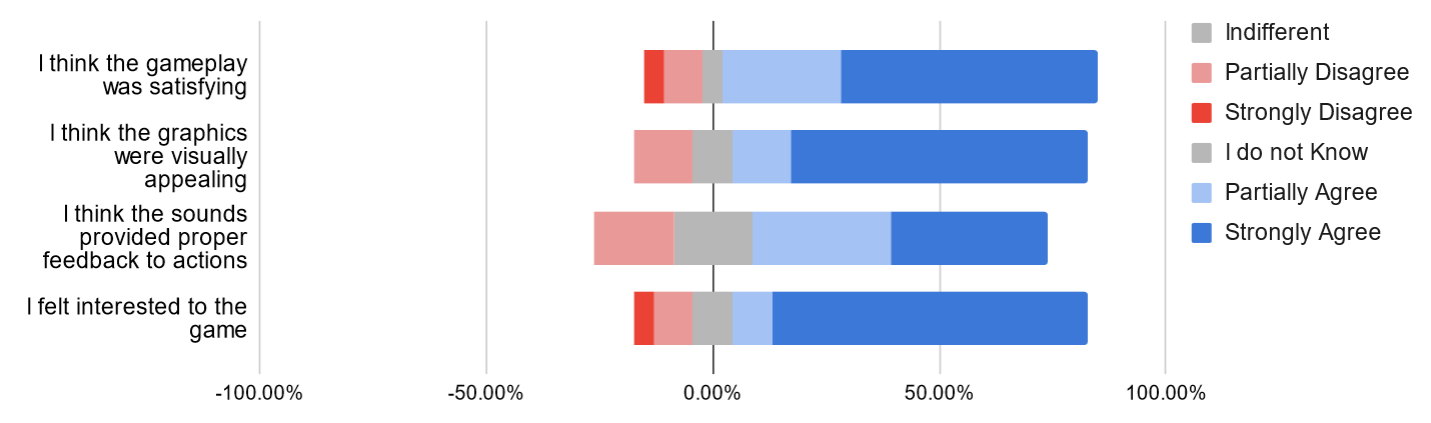
\includegraphics[width=36em]{figures/fig-perception-aesthetics-all-players.png}
        \legend{Source: Chart assembled by authors.}
        \label{fig:perception-aesthetics-all-players}
    \end{center}
\end{figure}

% About 90% of players strongly agreed that they were interested in the game
% About 90% players strongly agreed that the game was satisfying
% About 80% of players strongly agreed that the game was visually appealing, 
% About 90% of players thought the sounds harmonized with in-game occurrences
%   > We can assume there is no lack of interest or dislike based on aesthetical elements
Regarding player perceptions on their interest on the game and the game's aesthetics represented in Figure \ref{fig:perception-aesthetics-all-players}, about 90\% of the user base agreed that they were interested in the game. A similar percentage agreed that the game was satisfying to play, and that the in-game audio (sound effects) harmonized with in-game occurrences. About 80\% of players agreed that the game was visually appealling (regarding the quality of the graphics). Therefore, it can be reasonable to assume that there is no lack of interest or specific issues on the aesthetical elements of our implementation, and such elements should not affect the results of our user performance evaluation.

% Perceptions on Learning - All Players
% =======================
\begin{figure}[!ht]
    \begin{center}
    \caption{Perceptions on the ease of learning to play the game - All Players.}
        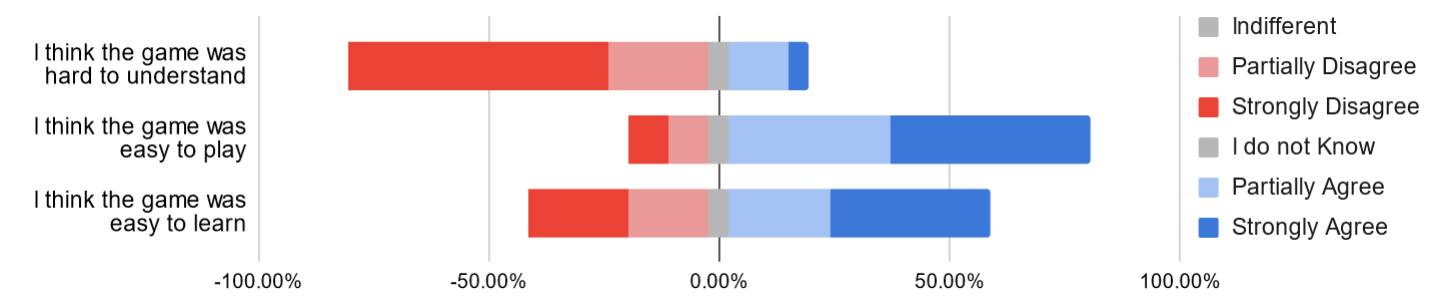
\includegraphics[width=36em]{figures/fig-perception-learning-all-players.png}
        \legend{Source: Chart assembled by authors.}
        \label{fig:perception-learning-all-players}
    \end{center}
\end{figure}

% 60% players strongly disagreed that the game was hard to understand, while the other 40% was mixed, partially agreeing, disagreeing or being indifferent
% Most players agreed that the game was easy to play
% Mixed opinions on the game being easy to learn, with strong opinions on both ends of the spectrum
%   > There might be a problem in the learning curve of the game's mechanics
Regarding player perceptions on the ease of learning how to play the game (by executing basic game mechanics) shown in Figure \ref{fig:perception-learning-all-players}, about 60\% of the player base strongly disagreed that the game was hard to understand, while the remaining 40\% had mixed opinions, by partially agreeing, partially disagreeing or being indifferent to the proposition. About 80\% of the player base agreed that the game was easy to playing regarding basic game mechanics.

The proposition regarding the game being easy to learn had mixed opinions, with a similar amount of strong agreement and disagreement. Therefore, there is an indication that there could be an issue with the game's learning curve regarding the use of basic mechanics, which would be an issue of level design where the order where challenges are presented to the player are unoptimal, and could affect their improvement process. This could affect player performance in the early levels of a first playthrough, where players are still not used to the game's mechanics and have to identify enemy patterns in parallel to learning basic game elements.

% Perceptions on Troubles - All Players
% =======================
\begin{figure}[!ht]
    \begin{center}
    \caption{Perceptions on issues when playing the game - All Players.}
        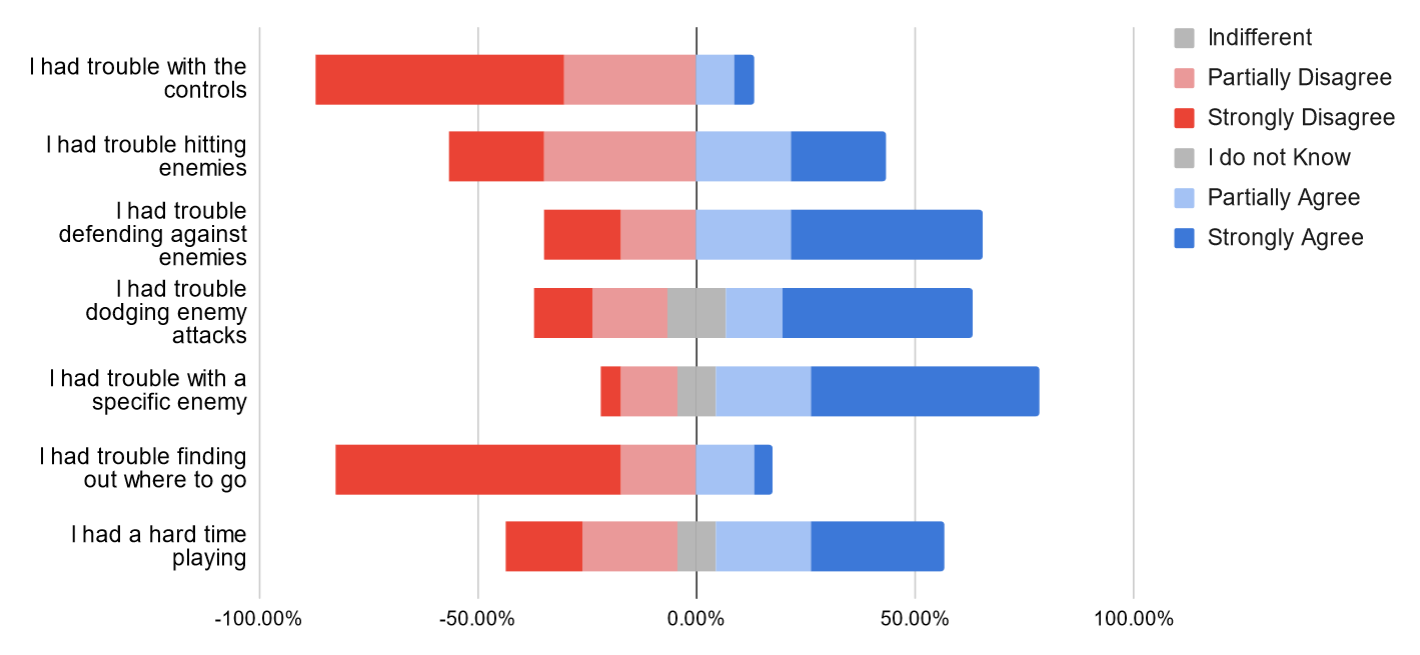
\includegraphics[width=36em]{figures/fig-perception-troubles-all-players.png}
        \legend{Source: Chart assembled by authors.}
        \label{fig:perception-troubles-all-players}
    \end{center}
\end{figure}

% Almost all players disagreed to have issues with the game's controls, with about 30% only partially disagreeing.
% Questions on hitting enemies, defending, dodging, specific enemy and "hard time playing" had mixed opinions, and could have been interpreted as difficulty-related.
% 90% did not find that they had issues finding out where to go
%   > Issues with formulating the questions
%   > Players did not have issues in finding out where to go.
Regarding player perceptions on issues identified when playing the game presented in figure \ref{fig:perception-troubles-all-players}, almost all players disagreed to have issues with the game's controls, with only about 30\% partially disagreeing. Propositions regarding the ability to hit enemies, defend against enemies and dodging enemy attacks had mixed opinions, with a slightly favorable perception on difficulty of performing defensive actions. About 90\% of players disagreed that they had issues finding out the path to level objectives.

Therefore, it is reasonable to assume that the design of input controls did not affect the ability of players to execute basic game mechanics, and that the level layouts provided a clear presentation of the path which should be taken by players. However, we identify an issue with the propositions regarding the ability to hit enemies, defending against enemies and dodging enemy attacks. Such propositions were formulated in a generalistic phrasing that could be interpreted as being related to the player's perception of difficulty, instead of the ability to execute each mechanic. Therefore, we could not consolidate a definite conclusion about the results of such propositions.

% Perceptions on Feelings - All Players
% =======================
\begin{figure}[!ht]
    \begin{center}
    \caption{Perceptions on feelings when playing the game - All Players.}
        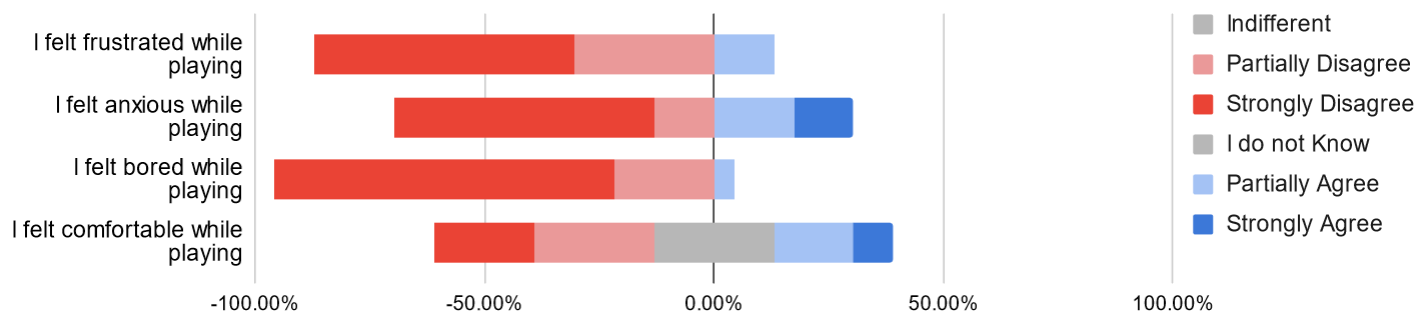
\includegraphics[width=36em]{figures/fig-perception-feelings-all-players.png}
        \legend{Source: Chart assembled by authors.}
        \label{fig:perception-feelings-all-players}
    \end{center}
\end{figure}

% Almost all players disagreed to have felt frustrated
% Most players disagreed to have felt anxious
% Almost all players disagreed to have felt bored
% Players had mixed opinions on feeling comfortable
%   > Short duration of the experiment might not have been enough to capture relevant affect-based data
%   > Players were receptive to dying and repeating levels
%   > Players were not bored when being defeated
Regarding player perceptions on affect-based propositions presented in figure \ref{fig:perception-feelings-all-players}, about 90\% of users disagreed to have felt frustrated when playing the game, with about 40\% only partially disagreeing with such proposition. About 80\% of players disagreed to have felt anxious while playing, and about 95\% of users disagreed to have felt bored whiel playing. Regarding feeling comfortable while playing, players had mixed opinions, with a slight tendency towards disagreeing with feeling comfortable.

We identify an issue with capturing affect-based metrics regarding the short duration of the experiment, which was devised to last in average 30 minutes of duration. In this short time frame, players might not be able to have sufficient information to assess whether they were affected positively or negatively by the game. However, with the current data we could still assume that boredom did not affect the performance players in the second playthrough, and that players were significantly receptive to being defeated and repeating the later levels on a playthrough.

% =================================================================
% =================================================================
% =================================================================

\subsection{Beginner Players}

% Describe and analyze possible causes for results in metrics for beginner players
% Verify global increase and decrease of metrics through charts (a) and (b)
% Compare the effects of dynamic difficulty on the learning curve through chart (c)
% Compare the level of challenge of dynamic through chart (d)
% Analyze the validity of the data through the standard deviation
In this section, we describe and analyze the observed results for each performance metric in the scope of beginner players. We attempt to verify the global increase and decrease of performance by analyzing charts \textsc{(a)} and \textsc{(b)} for each metric. We attempt to assess the effects of dynamic difficulty on the learning curve through chart \textsc{(c)} for each metric. We compare the level of challenge presented in the \nth{2} playthrough through chart \textsc{(d)}. Finally, we attempt to estimate the validity of the data through the general standard deviation of samples for each metric. A summarized version of the observations used as input for the analysis can be seen in Table \ref{tab:observations-performance-metrics-beginners}.

% Performance
% =============================

% Table with Observations for Performance Metrics for Beginner Players
\begin{table}[ht]
    \begin{center}
      \caption{Summarized observations on Performance Metrics for Beginner Players.}
      \label{tab:observations-performance-metrics-beginners}
      \rowcolors{2}{}{gray!25} % Alternate row colors
      \begin{tabular}{ >{\small}w{c}{6em} >{\footnotesize}w{l}{28em} } % alignments and column size
        \addlinespace
        \toprule
        % Headings
        \bf Metric & \bf Observations  \\
        \midrule
        % Data
        % ----------------------------------------------------------------
        \makecell[c]{Adjustment\\Targets\\Average} & 
        \makecell*[{{p{33em}}}]
        {
            \textbullet\space Significant increase in average target level for \nth{2} part in group A. Could show increased challenge level for \nth{2} playthrough; \\ % (a)
            \textbullet\space Steady increase towards intermediate fixed difficulty in \nth{1} part for group B (Dynamic Difficulty). Shows satisfactory learning curve; \\ % (b)
            \textbullet\space Low standard deviation in all observed results. % std deviation
        } \\
        % ----------------------------------------------------------------
        % Attack avoidance efficiency
        \makecell[c]{Attack\\Avoidance\\Efficiency} & 
        \makecell*[{{p{33em}}}]
        {
            \textbullet\space Globally higher efficiency in \nth{2} playthrough. Players seem to be more defensively efficient in a \nth{2} playthrough. \\ % global
            \textbullet\space Slightly higher efficiency in \nth{1} playthrough for players in Group B (Dynamic). Could show signs of a more efficient learning curve. \\ % (c)
            \textbullet\space Slightly less efficiency in the \nth{2} playthrough for Group A (Dynamic). Could be explained by a higher average difficulty on dynamic difficulty. \\ % (d)
            \textbullet\space Significant standard deviation in some of the samples. \\ % std deviation
        } \\
        % ----------------------------------------------------------------
        % Attack Window Efficiency
        \makecell[c]{Attack\\Window\\Efficiency} & 
        \makecell*[{{p{33em}}}]
        {
            \textbullet\space Globally higher efficiency in \nth{2} playthrough. Players seems to be more offensively efficient in a \nth{2} playthrough. \\ % global
            \textbullet\space Globally lower efficiency in level 3. Could be caused by the new enemy type introduced. \\ % global
            \textbullet\space Slightly higher efficiency in \nth{1} playthrough for Group B (Dynamic). Could represent a more efficient learning curve. \\ % (c)
            \textbullet\space Significantly lesser efficiency in \nth{2} playthrough for Group A (Dynamic). Could be caused by a more significative level of challenge. \\ % (d)
            \textbullet\space Significant standard deviation in some of the samples. \\ % std deviation
        } \\
        % ----------------------------------------------------------------
        % Completion time
        \makecell[c]{Completion\\Time} & 
        \makecell*[{{p{33em}}}]
        {
            \textbullet\space Steady global increase of completion time after each level. \\
            \textbullet\space Spike in global completion time (higher) in last level. \\
            \textbullet\space Slightly lower global completion times in \nth{2} playthrough. \\
            \textbullet\space Slightly lower Group B (Dynamic) completion times in \nth{1} playthrough. Significant decrease in 4th level. \\
            \textbullet\space Slightly higher Group A (Dynamic) completion times in \nth{2} playthrough. Higher level of challenge from adjustments. \\
            \textbullet\space Significant difference in completion times in \nth{4} level between Groups A and B. \\
            \textbullet\space Low standard deviation in most samples. \\ % std deviation
        } \\
        % ----------------------------------------------------------------
        % Damage Dealth per 10 seconds
        \makecell[c]{Damage Dealt\\per 10 seconds} & 
        \makecell*[{{p{33em}}}]
        {
            \textbullet\space Globally higher damage dealt in \nth{2} playthrough. \\ % global
            \textbullet\space Globally lower damage dealt in \nth{3} level. Could be mapped to a difficulty spike. \\ % global
            \textbullet\space Slightly higher damage dealt in \nth{1} playthrough by Group B (Dynamic). Higher contrast in \nth{3} level. Could show the effects of learning curve. \\ % (c)
            \textbullet\space Mixed results on damage dealt in \nth{2} playthrough between both groups. \\ % (d)
            \textbullet\space A few isolated samples present a significant standard deviation. \\ % std deviation
        } \\
        % ----------------------------------------------------------------
        % Deaths per Level
        \makecell[c]{Deaths per\\Level} & 
        \makecell*[{{p{33em}}}]
        {
            \textbullet\space Global decrease in deaths in \nth{2} playthrough. \\ % global
            \textbullet\space Decrease in \nth{2} playthrough for Group B (Fixed) is much more significant than group A. Could be an effect of a more efficient learning curve. \\ % (b)
            \textbullet\space Similar number of deaths in \nth{1} playthrough for both groups. \\ % (c)
            \textbullet\space Significantly higher average of deaths in Group A (Dynamic) \nth{2} playthrough. Could be an effect of increased level of challenge. \\ % (d)
            \textbullet\space High standard deviation in samples for later levels. Could show issues with learning curve. \\ % std deviation
        } \\
        % ----------------------------------------------------------------
        % Health Lost per Encounter
        \makecell[c]{Health Lost\\per Encounter} & 
        \makecell*[{{p{33em}}}]
        {
            \textbullet\space Significantly lower global damage taken in \nth{2} playthrough. Players are more defensively efficient. \\ % global
            \textbullet\space Significantly lower decrease of damage taken in Group B \nth{2} playthrough. Could correlate with learning curve. \\ % (b)
            \textbullet\space Similar amount of damage taken between groups in \nth{1} playthrough. \\ % (c)
            \textbullet\space Significantly higher amount of damage taken in Group A (Dynamic) in \nth{2} playthrough. Correlates with level of challenge. \\ % (d)
            \textbullet\space High standard deviation in Group B \nth{1} playthrough. \\ % std deviation
        } \\
        % ----------------------------------------------------------------
        \bottomrule
      \end{tabular}
    \end{center}
\end{table}

%adjustment_target_level
% Avg Adjustment Target per Level - Beginners
% =======================
\begin{figure}[ht]
    \begin{center}
    \caption{Avg. Adjustment Targets Average (Y) per Level (X) for Beginners.}
        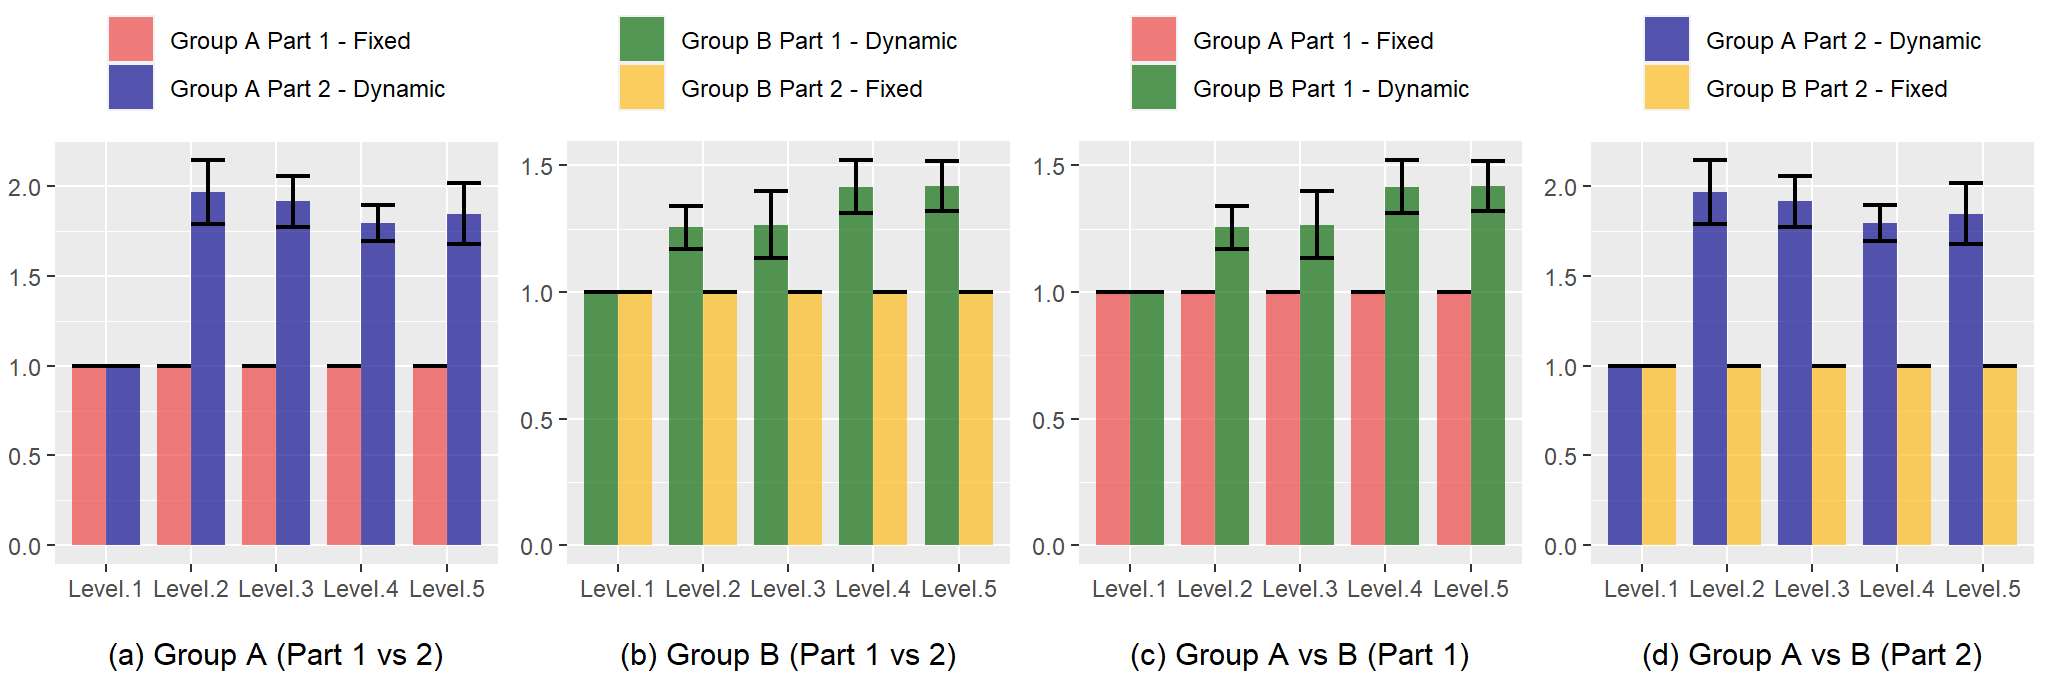
\includegraphics[width=\textwidth]{figures/adjustment_target_level-beginner_players.png}
        \legend{Source: Assembled by authors.}
        \label{fig:result-metric-beginners-adjustment-target-level}
    \end{center}
\end{figure}

Regarding the \emph{Adjustment Targets Average}, which can be analyzed in Figure \ref{fig:result-metric-beginners-adjustment-target-level}, we noticed a significant increase in the average adjustment level in the second playthrough for players in Group A, which played the Fixed Difficulty version first and the Dynamic Difficulty version second. As this metric represents the average target difficulty for each of the adjustments, we can compare the results to the fixed presets for the intermediate difficulty. Through this comparison, we can infer that beginner players were able to sufficiently learn the game mechanics and enemy behavioral patterns, and would be able to complete the game at the presets for the intermediate difficulty.

We also noticed a steady increase in adjustment targets during the first playthrough for players in Group B, which played the Dynamic Difficulty version first. This could reinforce the idea that players steadily learned and improved upon their execution of game mechanics, as the DDA system inferred that the performance of players was generally above the thresholds for presets for the beginner difficulty. All results showed an acceptable standard deviation, to which we can conclude that the results appropriately represent the beginner players group. 

%attack_avoidance_efficiency
% Avg Attack Avoidance Efficiency per Level - Beginners
% =======================
\begin{figure}[ht]
    \begin{center}
    \caption{Avg. Attack Avoidance Efficiency (Y) per Level (X) for Beginners.}
        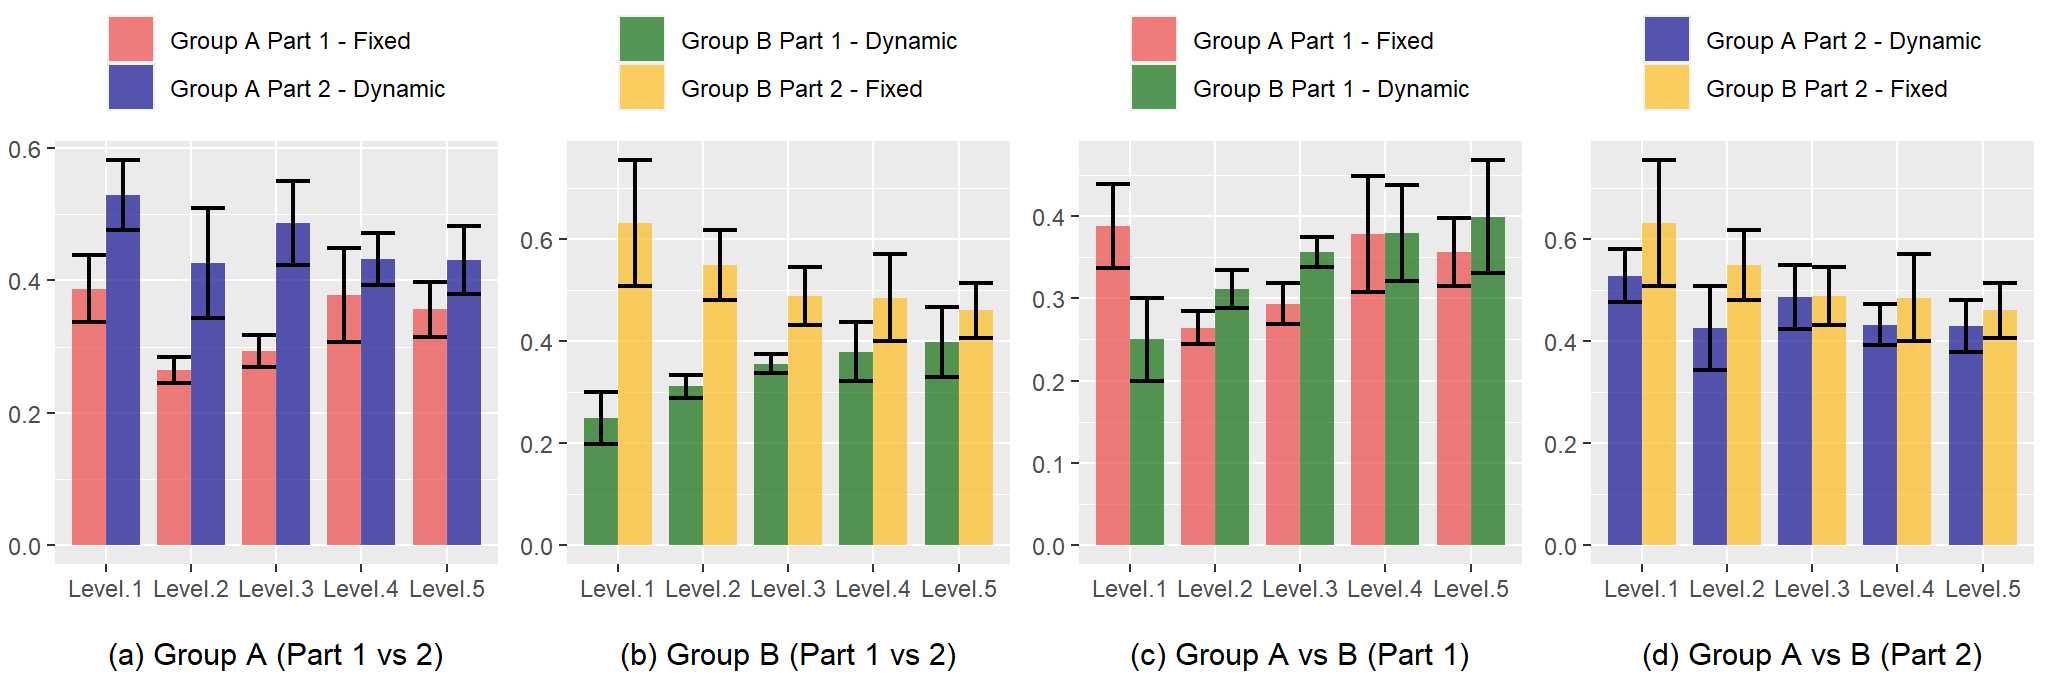
\includegraphics[width=\textwidth]{figures/attack_avoidance_efficiency-beginner_players.png}
        \legend{Source: Assembled by authors.}
        \label{fig:result-metric-beginners-attack-avoidance-efficiency}
    \end{center}
\end{figure}

Regarding the efficiency of avoiding enemy attacks, which can be analyzed in Figure \ref{fig:result-metric-beginners-attack-avoidance-efficiency}, we noticed a significantly higher efficiency for both groups in the second playthrough. In general, players seem to be better at defending themselves in the second playthrough, where they would have learned all basic game mechanics and general enemy behaviors. We also noticed a slightly higher efficiency in the first playthrough after the second level for players in Group B, which played the Dynamic Difficulty version first. This could be related to a more efficient learning curve, where players which are presented to tougher challenges first might be able to defend themselves better in the later levels.

We noticed a reduced efficiency in the second playthrough for Group A, which played the Dynamic Difficulty version second. By relating this metric with the \emph{Adjustment Targets Average}, we can infer that a higher degree of challenge had a negative impact on the ease at which a player was able to dodge attacks. This can be related with the fact that in higher difficulties the player will often engage combat against a larger amount of enemies simultaneously, which could make dodging attacks harder. We identified a significant standard deviation in some of the samples, and particularly in the first part of the experiment.

%attack_window_efficiency
% Avg Attack Window Efficiency per Level - Beginners
% =======================
\begin{figure}[ht]
    \begin{center}
    \caption{Avg. Attack Window Efficiency (Y) per Level (X) for Beginners.}
        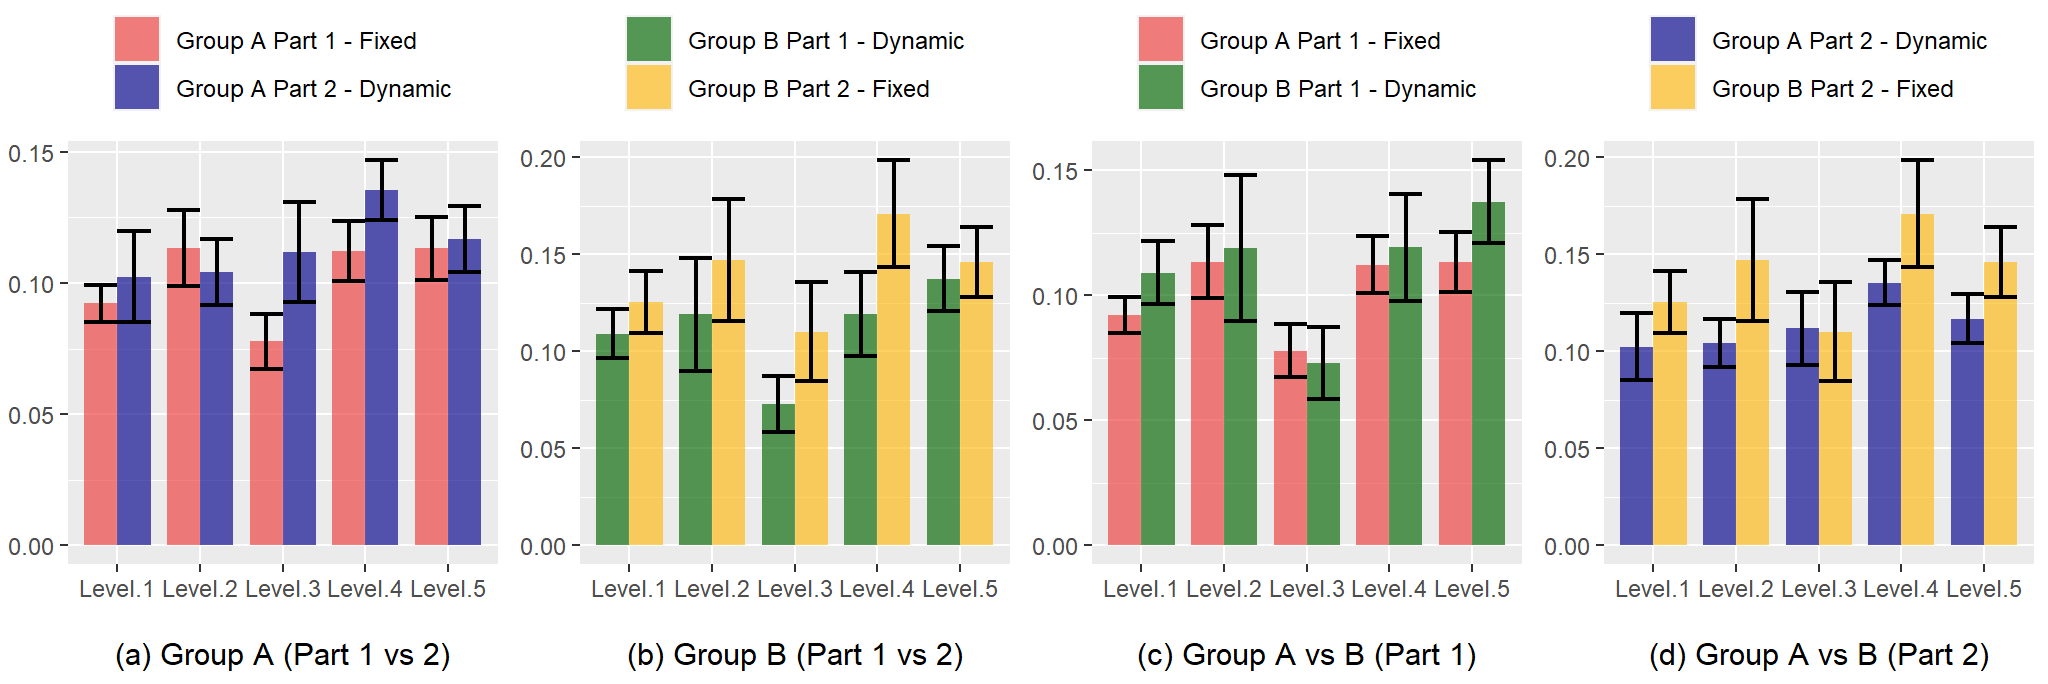
\includegraphics[width=\textwidth]{figures/attack_window_efficiency-beginner_players.png}
        \legend{Source: Assembled by authors.}
        \label{fig:result-metric-beginners-attack-window-efficiency}
    \end{center}
\end{figure}

Regarding the efficiency of dealing damage to enemies when they are vulnerable through the \emph{Attack Window Efficiency} metric, which can be analyzed in Figure \ref{fig:result-metric-beginners-attack-window-efficiency}, we noticed a higher efficiency in the second playthrough for both groups. Players seemed to be better at taking advantage of enemy vulnerabilities, such as staggers or attack cooldowns. This could be related to the players understanding that after an enemy performs an attack, they have a cooldown time before performing another. However, we also noticed a lower efficiency for both groups in level 3, which correlates with the introduction of the \emph{Armored Knight} enemy, which is designed to be the hardest enemy in the game.

We also noticed a slightly higher efficiency in the first playthrough for Group B, which plays the Dynamic Difficulty version of the application first, and particularly in levels 4 and 5. This reinforces our previous idea that Dynamic Difficulty presents a more efficient learning curve for understanding strategies. In the second playthrough, players from Group A, which played the Fixed Difficulty version first, had a significantly lesser efficiency in taking advantage of attack windows. This could be related to an increase level of challenge, where the player has to tackle larger enemy groups simultaneously. We noticed a significant standard deviation in some of the samples.

%completion_time
% Avg Completion Time per Level - Beginners
% =======================
\begin{figure}[ht]
    \begin{center}
    \caption{Avg. Completion Time (Y) per Level (X) for Beginners.}
        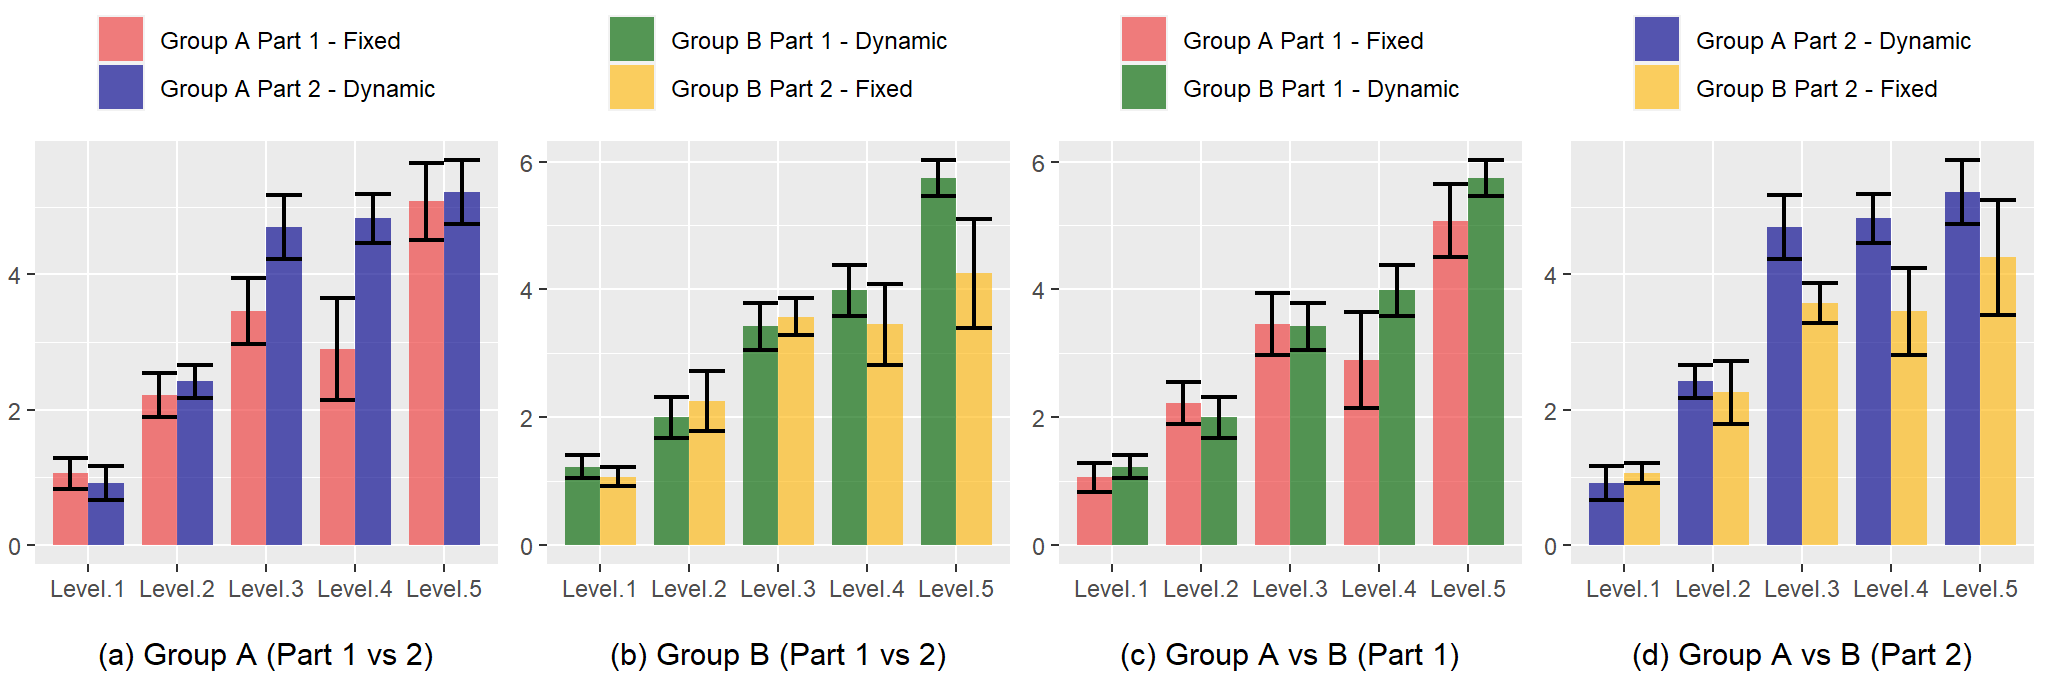
\includegraphics[width=\textwidth]{figures/completion_time-beginner_players.png}
        \legend{Source: Assembled by authors.}
        \label{fig:result-metric-beginners-completion-time}
    \end{center}
\end{figure}

Regarding the average time beginner players took to complete which level, which can be analyzed in Figure \ref{fig:result-metric-beginners-completion-time}, we noticed slight but continuous increase of completion time for both groups with each level, which correlates with our intented level design and experiment duration. However, we noticed a spike in the completion time for both groups in the last level, which took significantly longer to complete. During the design stage, we devised the last level to take about the same duration as the fourth level. This could signify either an unexpected increase in the difficulty, or an issue with the level layout.

We also noticed slightly lower level completion times for both groups during the second playthrough, which aligns with the previously observed efficiency when dealing with enemies. Additionally, since the level layout might be the same depending on the adjustment target, this could also be related to the player being used to such level layout. In Group B, which plays the Dynamic Difficulty version first, we noticed slightly lower completion times during the first playthrough, with the exception of a significant decrease in the fourth level. This could also reinforce differences in the learning curve and efficiency of players which learn to play in a DDA system.

Group A had slightly higher completion times during the second playthrough, in which they would play the DDA version of the application. This could be caused by a generally higher level of challenge caused by the adjustment targets, where a higher amount of enemies, higher enemy difficulty and a different level layout could significantly affect the performance of players. Additionally, there was a significant difference in completion times for the fourth level during the second playthrough when comparing Group A to Group B, where group B was had considerably lower completion times. This could be explained by the fact that Group B experienced the Fixed Difficulty version second, which had beginner-level adjustment targets -- and thus players which were already accustomed to game mechanics would find the level of challenge to be low. We found there was a low standard deviation in almost all samples for this metric.

%damage_dealt_per_10s
% Avg Damage Dealt per 10s per Level - Beginners
% =======================
\begin{figure}[ht]
    \begin{center}
    \caption{Avg. Damage Dealt per 10 seconds (Y) per Level (X) for Beginners.}
        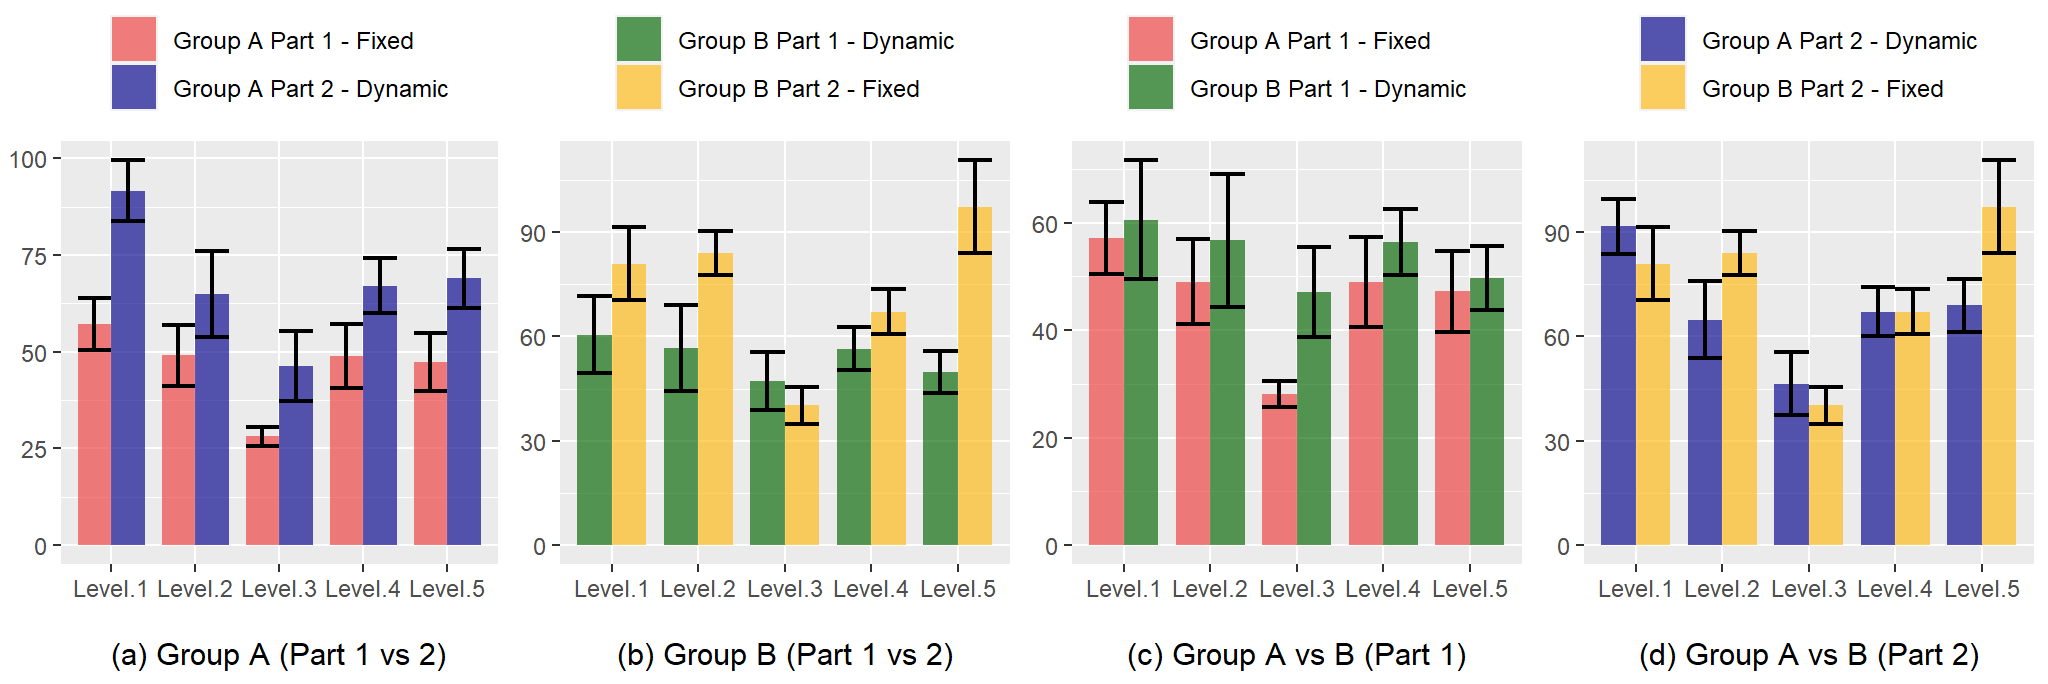
\includegraphics[width=\textwidth]{figures/damage_dealt_per_10s-beginner_players.png}
        \legend{Source: Assembled by authors.}
        \label{fig:result-metric-beginners-damage-dealt-per-10s}
    \end{center}
\end{figure}

Regarding the average damage dealt by players during combat, which is represented by the \emph{Damage Dealt per 10 seconds} metric and can be analyzed in Figure \ref{fig:result-metric-beginners-damage-dealt-per-10s}, we noticed that both groups dealt a significantly higher amount of damage during the second playthrough. In general, it could be inferred that players were much more efficient offensively, and our findings harmonize with the results for the \emph{Attack Window Efficiency} metric. However, we noticed a lower amount of damage dealt during the third level for both groups. This could be related to a difficulty spike, which could be caused by the introduction of the \emph{Armored Knight} enemy.

We also noticed a slightly higher amount of damage dealt in the first playthrough by Group B in comparison to Group A, with a higher contrast during the third level. This reinforces the hypothesis of a more efficient learning curve during first playthroughs on DDA systems. However, we had mixed results on the damage dealt during the second playthrough for both groups, which leads to no conclusion regarding the level of challenge presented by DDA systems on a second playthrough. A few isolated samples of this metric had a large standard deviation.

%deaths_per_level
% Avg Deaths per Level - Beginners
% =======================
\begin{figure}[ht]
    \begin{center}
    \caption{Avg. Deaths (Y) per Level (X) for Beginners.}
        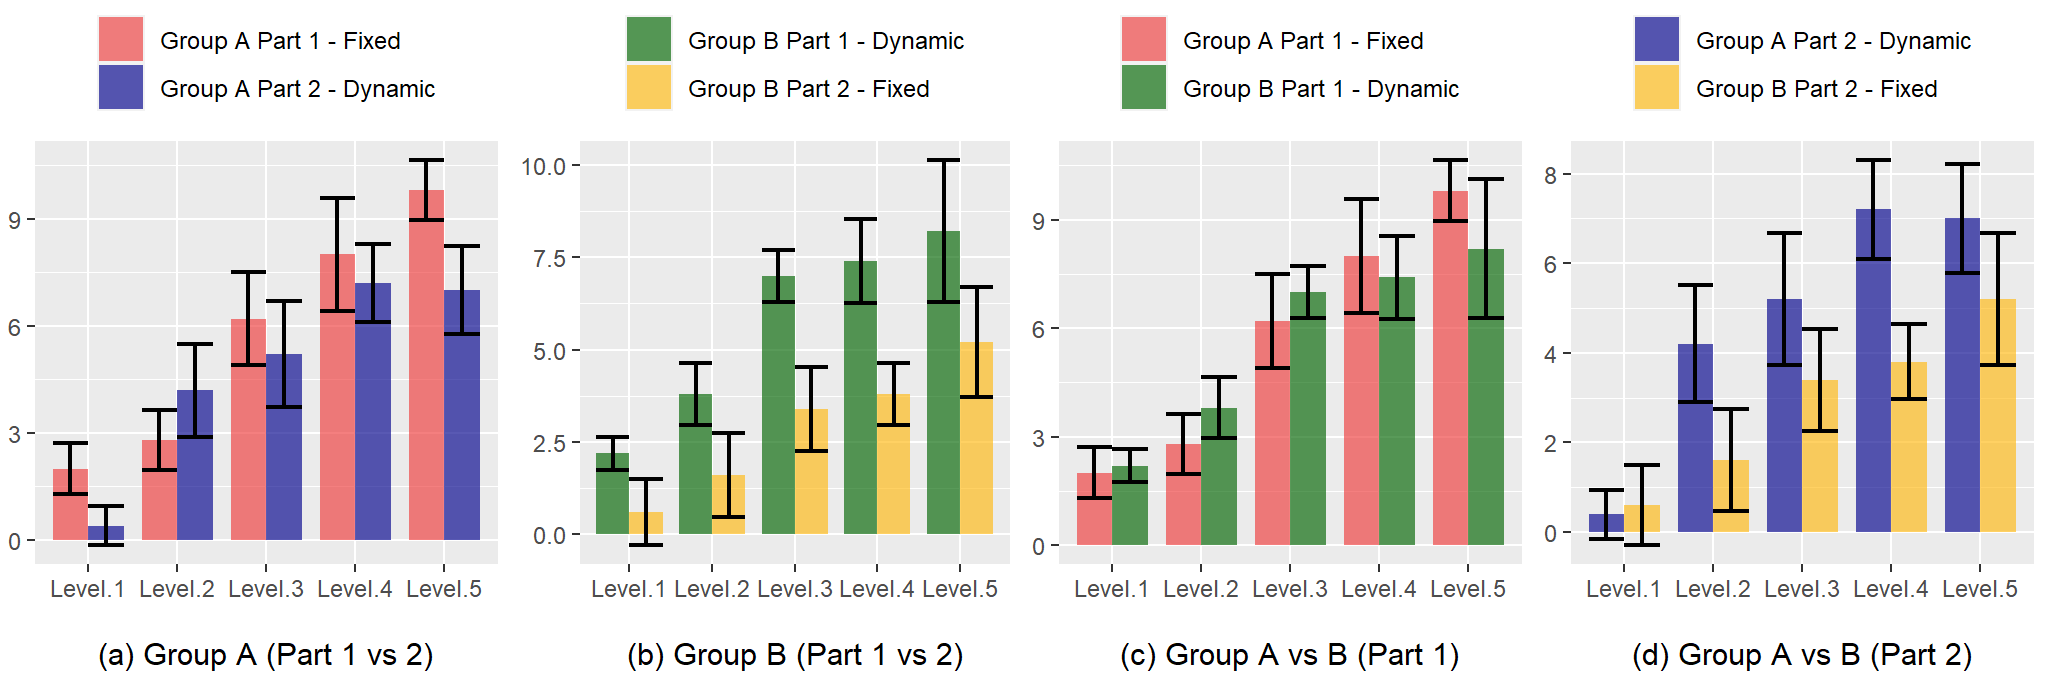
\includegraphics[width=\textwidth]{figures/deaths_per_level-beginner_players.png}
        \legend{Source: Assembled by authors.}
        \label{fig:result-metric-beginners-deaths-per-level}
    \end{center}
\end{figure}

Regarding the average number of deaths at each level, which can be analyzed in Figure \ref{fig:result-metric-beginners-deaths-per-level}, we noticed a significant decrease in the number of deaths for both groups during the second playthrough. However, the decrease for Group B (which plays the Fixed Difficulty version second) is much more significant than Group A, which reinforces the fact that the Dynamic Difficulty version presented a much more adequate challenge level for players on a second playthrough. Additionally, we could infer that the learning curve for players which played the DDA version first was more effective.

During the first playthrough, we noticed a similar number of deaths for both groups, with a slight decrease in the number of deaths at the fourth and fifth level for players who played the DDA version first. We also observed a significantly higher number of deaths in the second playthrough for Group A, which played the Dynamic Difficulty version second. This could be a representative of the increased level of challenge of Dynamic Difficulty at a second playthrough. We also noticed a high standard deviation in the samples for later levels, which could show issues with level design or the learning curve.

%health_lost_per_encounter
% Avg Health Lost per Encounter per Level - Beginners
% =======================
\begin{figure}[ht]
    \begin{center}
    \caption{Avg. Health Lost per Encounter (Y) per Level (X) for Beginners.}
        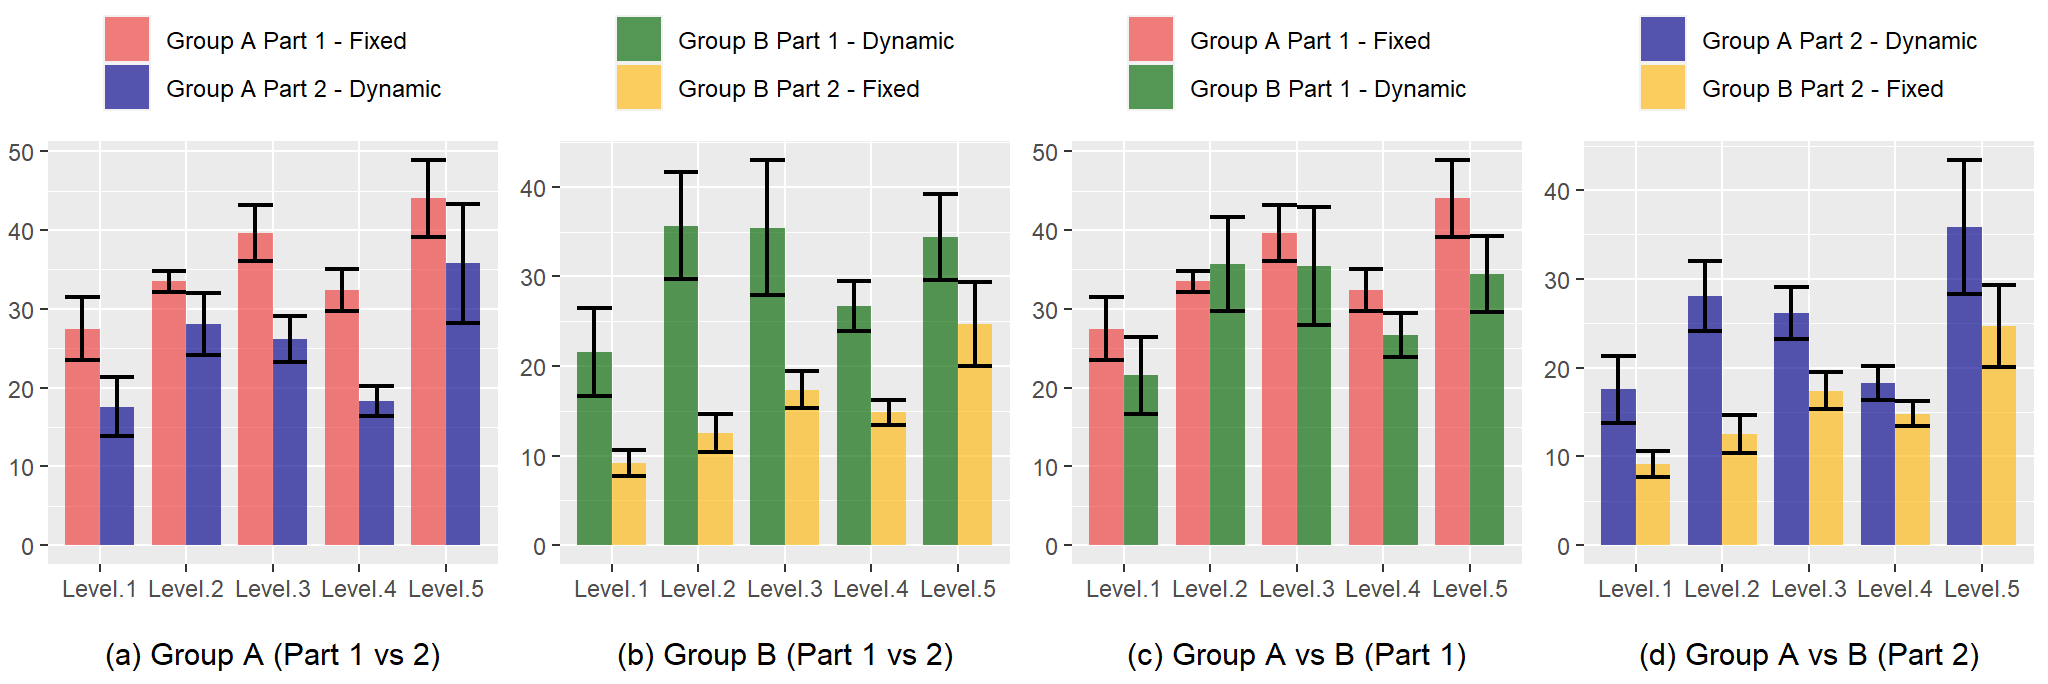
\includegraphics[width=\textwidth]{figures/health_lost_per_encounter-beginner_players.png}
        \legend{Source: Assembled by authors.}
        \label{fig:result-metric-beginners-health-lost-per-encounter}
    \end{center}
\end{figure}

Regarding the amount of health lost during combat, which is represented by the \emph{Health Lost per Encounter} metric and can be analyzed through Figure \ref{fig:result-metric-beginners-health-lost-per-encounter}, we noticed a significant decrease of damage taken for both groups in a second playthrough, which reinforces our previous observation that players are more defensively efficient during a second playthrough, where they would have learned all basic game mechanics and enemy behavioral patterns.

During the second playthrough, we noticed a significantly lower damage taken by Group B in comparison to Group A, which could correlate with the learning curve by starting with a Dynamic Difficulty version first, and playing an easier version of the game second. We noticed a similar amount of damage taken by both groups in the first playthrough, which correlates with the observed results for the number of deaths. We also noticed a significantly higher amount of damage taken in group A in the second playthrough when comparing to Group B, which correlates with the level of challenge presented in a DDA system at a second playthrough. We noticed a high standard deviation in the samples for the first playthrough of Group B.

% Perceptions
% =============================

% Perceptions on Difficulty -- Beginner Players
% =======================
\begin{figure}[ht]
    \begin{center}
    \caption{Perceptions on Difficulty - Beginner Players.}
        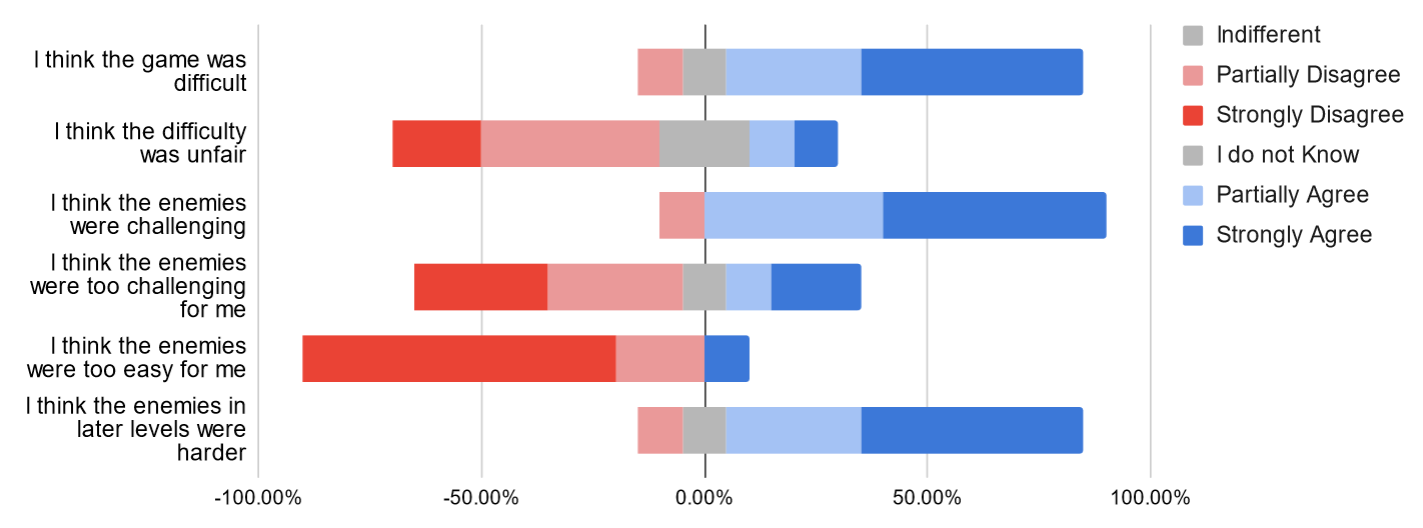
\includegraphics[width=36em]{figures/fig-perception-difficulty-beginner-players.png}
        \legend{Source: Chart assembled by authors.}
        \label{fig:perception-difficulty-beginner-players}
    \end{center}
\end{figure}

Regarding the perceptions of beginner players on game difficulty, which can be analyzed in Figure \ref{fig:perception-difficulty-beginner-players}, most users perceived the game as being difficult, with about 50\% strongly aggreing and 30\% partially agreeing. About 70\% of players did not perceive the difficulty as being unfair, but 40\% only partially disagreed with the proposition. Therefore, we can assume that a more granular analysis on each specific group could have exposed issues regarding the level of challenge presented to players.

About 90\% of players perceived the enemies to be challenging, with 50\% strongly agreeing to such proposition. Most players found that the enemies were not overtly challenging regarding their skill level, but about 20\% disagreed. About 90\% of players disagreed that the enemies were too easy in comparison to their skill level, and 80\% of players felt that the enemies in the later levels were harder. Since enemy encounters in later levels were in fact designed to be more difficult, it is reasonable to infer that there are no relevant issues regarding the balancing of enemies for beginner players. 

% Perceptions on Learning -- Beginner Players
% =======================
\begin{figure}[ht]
    \begin{center}
    \caption{Perceptions on Learning - Beginner Players.}
        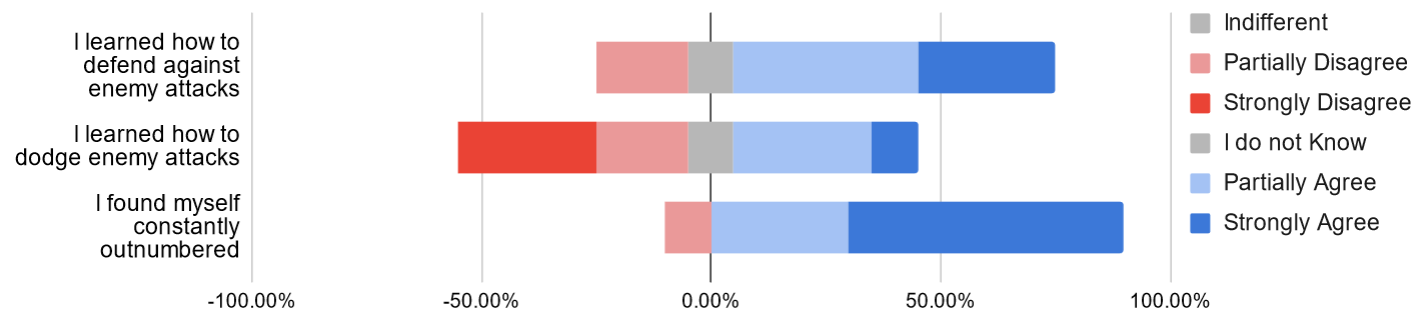
\includegraphics[width=36em]{figures/fig-perception-learning-beginner-players.png}
        \legend{Source: Chart assembled by authors.}
        \label{fig:perception-learning-beginner-players}
    \end{center}
\end{figure}

Regarding the perceptions of beginner players on learn basic mechanics of the game, which can be analyzed in Figure \ref{fig:perception-learning-beginner-players}, most users felt like they learned how to defend (block) against enemy attacks, with about 50\% only partially agreeing to such proposition. Mixed opinions were observed regarding the dodging mechanic, where 30\% of beginners strongly felt that they did not learn how to dodge. Additionally, 90\% of players felt like they were constantly outnumbered, with about 60\% strongly agreeing with such proposition. These results could show that beginner players were unable to properly learn the dodge mechanic. Additionally, we had strong indications that beginner players did not properly learn how to isolate their targets when engaging in combat.

% Perceptions on Playthroughs -- Beginner Players Group A
% =======================
\begin{figure}[ht]
    \begin{center}
    \caption{Perceptions on Playthroughs - Beginner Players Group A.}
        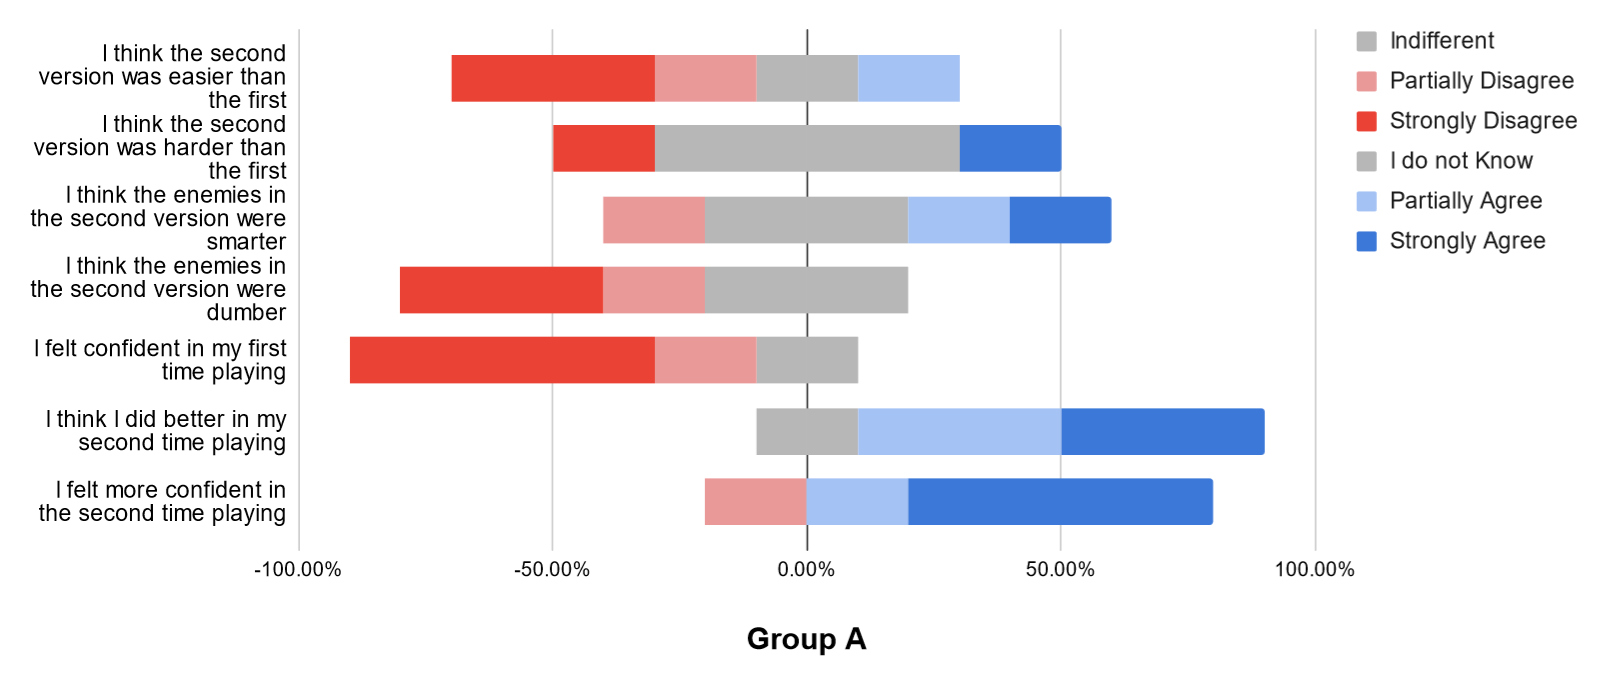
\includegraphics[width=36em]{figures/fig-perception-versions-beginner-players-group-a.png}
        \legend{Source: Chart assembled by authors.}
        \label{fig:perception-playthrough-beginner-players-group-a}
    \end{center}
\end{figure}

Regarding the perceptions of beginner players from Group A when comparing the first to the second playthrough, which can be analyzed in Figure \ref{fig:perception-playthrough-beginner-players-group-a}, about 80\% of players disagreed that the second version was easier than the first, and 80\% of players agreed that the second version was harder than the first. These results align with the fact that players in Group A experienced a higher challenge level in the second version caused by the adjustments performed by the dynamic difficulty.

About half of the beginner players were unable to tell whether the enemies in the second version were smarter, with an additional 30\% of players being agreeable to such proposition. Most players disagreed with the enemies in the second version being less intelligent, with about 40\% not being able to tell the difference. These results can be interpreted as some of the beginner players in Group A being able to perceive that the enemies in the Dynamic Difficulty version did in fact present a more sophisticated behaviors, with different attack patterns and decision algorithms.

About 80\% of players disagreed with feeling confident in their first playthrough, and 80\% of players felt like they performed better during their second playthrough. Additionally, 80\% of players also felt more confident during their second playthrough. Such perceptions align with the results seen in our performance metrics, where even though the level of challenge presented to players was higher, players were able to tackle enemies and execute game mechanics more efficiently.

% Perceptions on Playthroughs -- Beginner Players Group B
% =======================
\begin{figure}[ht]
    \begin{center}
    \caption{Perceptions on Playthroughs - Beginner Players Group B.}
        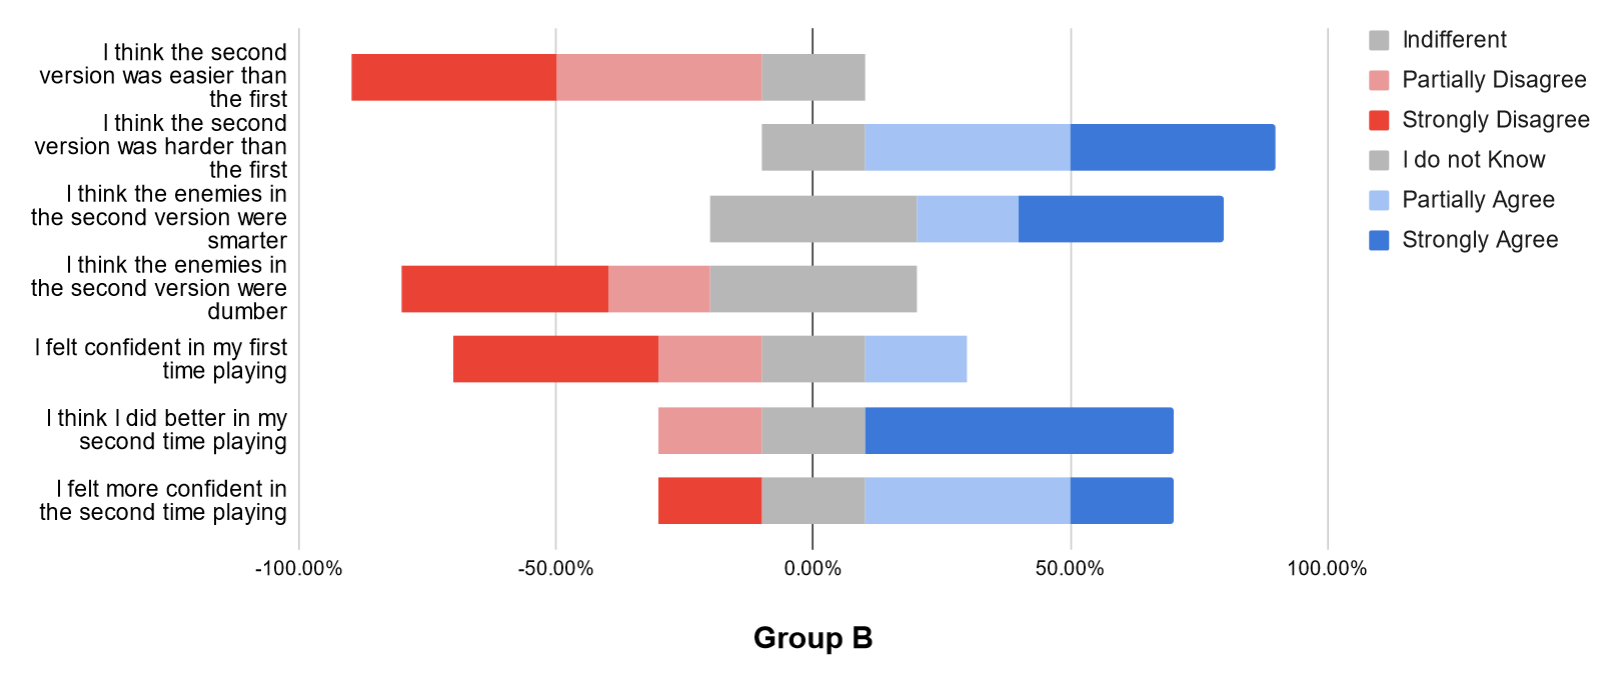
\includegraphics[width=36em]{figures/fig-perception-versions-beginner-players-group-b.png}
        \legend{Source: Chart assembled by authors.}
        \label{fig:perception-playthrough-beginner-players-group-b}
    \end{center}
\end{figure}

Regarding the perceptions of beginner players from Group B when comparing the first to the second playthrough, which can be analyzed in Figure\ref{fig:perception-playthrough-beginner-players-group-b}, about 70\% of players did not agree with the proposition that the second version of the game (Dynamic difficulty) was easier than the first. The other 30\% of players had partially agreeable or indifferent opinions. Most players were indifferent or did not know whether the second version was harder than the first, with the other 20\% either strongly agreeing or disagreeing. These results could be interpreted as players not being able to recognize the difference in difficulty between the two versions, even though players in Group B experienced a significantly easier level of challenge, as previously observed.

About 60\% of players felt like enemies in the second version were smarter than the first, with 40\% being unable to tell the difference. Most players disagreed that enemies in the second version were less intelligent, with 40\% being unable to assess the validity of the proposition. These results go in disagreement with the performance results regarding adjustment target values, where the overall game difficulty was observed to be lower in the second playthrough for players in Group B.

About 60\% of players disagreed with feeling confident in their first playthrough, with 40\% presenting indifferent or partially agreeable opinions. Similarly, 60\% of players perceived their performance on the second playthrough to be better, with 40\% partially agreeing to feeling more confident on a second playthrough. These results align with the previously seen performance results for group B, which were observed to be significantly higher than the first part of the experiment.

% ==================================================
% ==================================================
% ==================================================

\subsection{Intermediate Players}

% TODO write paragraphs

% Performance
% =============================

% Table with Observations for Performance Metrics for Intermediate Players
\begin{table}
    \begin{center}
      \caption{Summarized observations on Performance Metrics for Intermediate Players.}
      \label{tab:observations-performance-metrics-intermediates}
      \rowcolors{2}{}{gray!25} % Alternate row colors
      \begin{tabular}{ >{\small}w{c}{6em} >{\footnotesize}w{l}{25em} } % alignments and column size
        \addlinespace
        \toprule
        % Headings
        \bf Metric & \bf Observations  \\
        \midrule
        % Data
        % ----------------------------------------------------------------
        \makecell[c]{Adjustment\\Targets\\Average} & 
        \makecell*[{{p{30em}}}]
        {
            \textbullet\space Observation 1. \\
            \textbullet\space Observation 2. \\
            \textbullet\space Observation 3. \\
        } \\
        % ----------------------------------------------------------------
        % Attack avoidance efficiency
        \makecell[c]{Attack\\Avoidance\\Efficiency} & 
        \makecell*[{{p{30em}}}]
        {
            \textbullet\space Observation 1. \\
            \textbullet\space Observation 2. \\
            \textbullet\space Observation 3. \\
        } \\
        % ----------------------------------------------------------------
        % Attack Window Efficiency
        \makecell[c]{Attack\\Window\\Efficiency} & 
        \makecell*[{{p{30em}}}]
        {
            \textbullet\space Observation 1. \\
            \textbullet\space Observation 2. \\
            \textbullet\space Observation 3. \\
        } \\
        % ----------------------------------------------------------------
        % Completion time
        \makecell[c]{Completion\\Time} & 
        \makecell*[{{p{30em}}}]
        {
            \textbullet\space Observation 1. \\
            \textbullet\space Observation 2. \\
            \textbullet\space Observation 3. \\
        } \\
        % ----------------------------------------------------------------
        % Damage Dealth per 10 seconds
        \makecell[c]{Damage Dealt\\per 10 seconds} & 
        \makecell*[{{p{30em}}}]
        {
            \textbullet\space Observation 1. \\
            \textbullet\space Observation 2. \\
            \textbullet\space Observation 3. \\
        } \\
        % ----------------------------------------------------------------
        % Deaths per Level
        \makecell[c]{Deaths per\\Level} & 
        \makecell*[{{p{30em}}}]
        {
            \textbullet\space Observation 1. \\
            \textbullet\space Observation 2. \\
            \textbullet\space Observation 3. \\
        } \\
        % ----------------------------------------------------------------
        % Health Lost per Encounter
        \makecell[c]{Health Lost\\per Encounter} & 
        \makecell*[{{p{30em}}}]
        {
            \textbullet\space Observation 1. \\
            \textbullet\space Observation 2. \\
            \textbullet\space Observation 3. \\
        } \\
        % ----------------------------------------------------------------
        \bottomrule
      \end{tabular}
    \end{center}
\end{table}

%adjustment_target_level
% Avg Adjustment Target per Level - Intermediates
% =======================
\begin{figure}[!ht]
    \begin{center}
    \caption{Avg. Adjustment Targets Average (Y) per Level (X) for Intermediates.}
        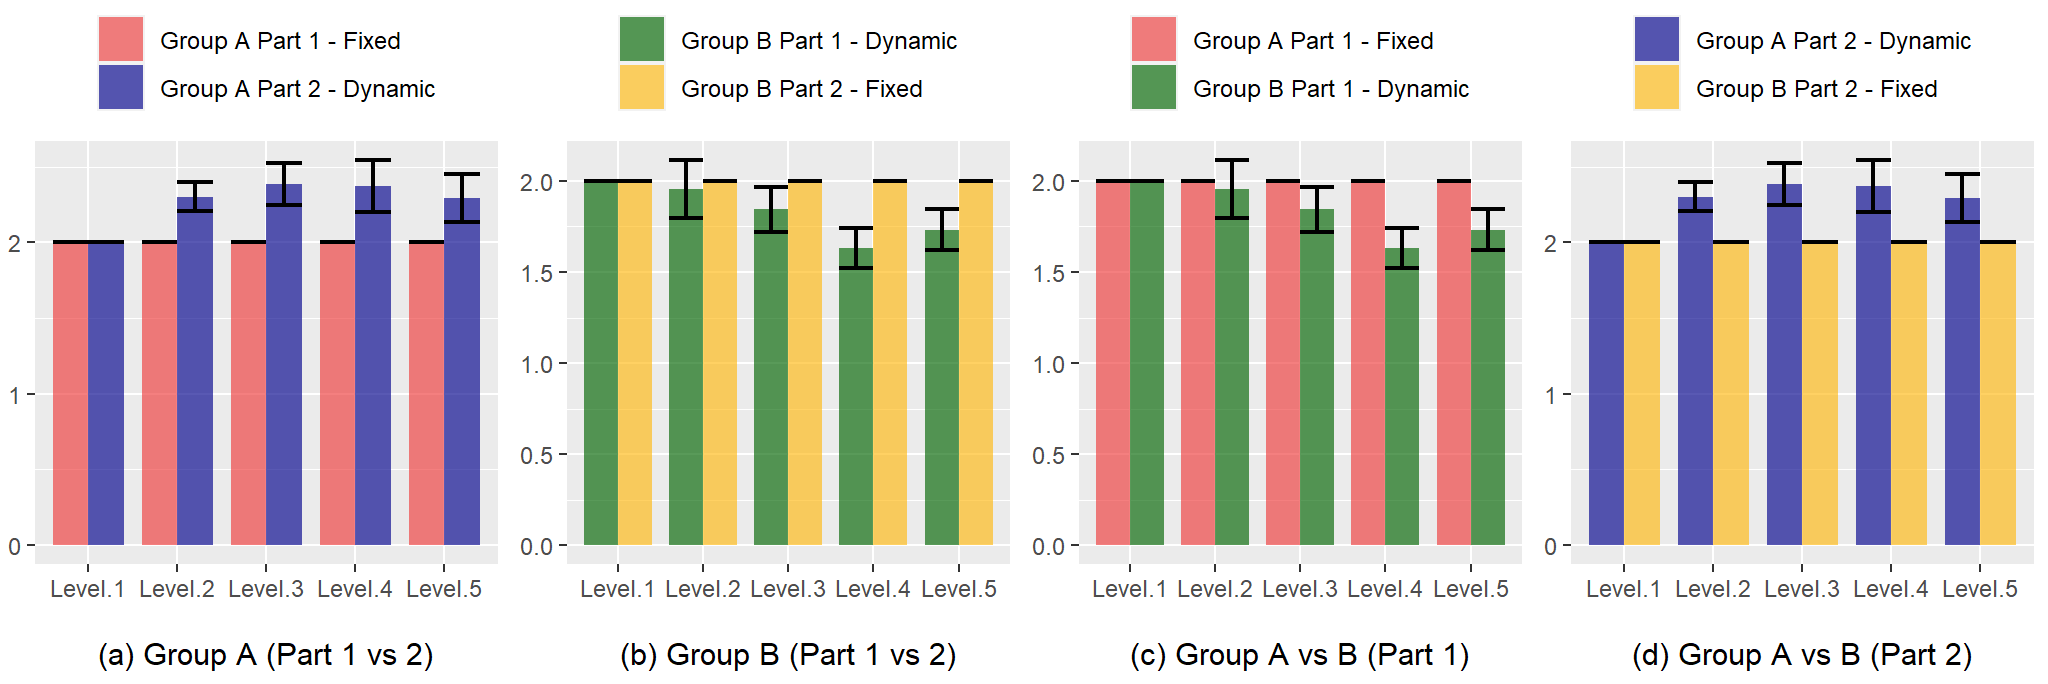
\includegraphics[width=\textwidth]{figures/adjustment_target_level-intermediate_players.png}
        \legend{Source: Assembled by authors.}
        \label{fig:result-metric-intermediate-adjustment-target-level}
    \end{center}
\end{figure}

%attack_avoidance_efficiency
% Avg Attack Avoidance Efficiency per Level - Intermediates
% =======================
\begin{figure}[!ht]
    \begin{center}
    \caption{Avg. Attack Avoidance Efficiency (Y) per Level (X) for Intermediates.}
        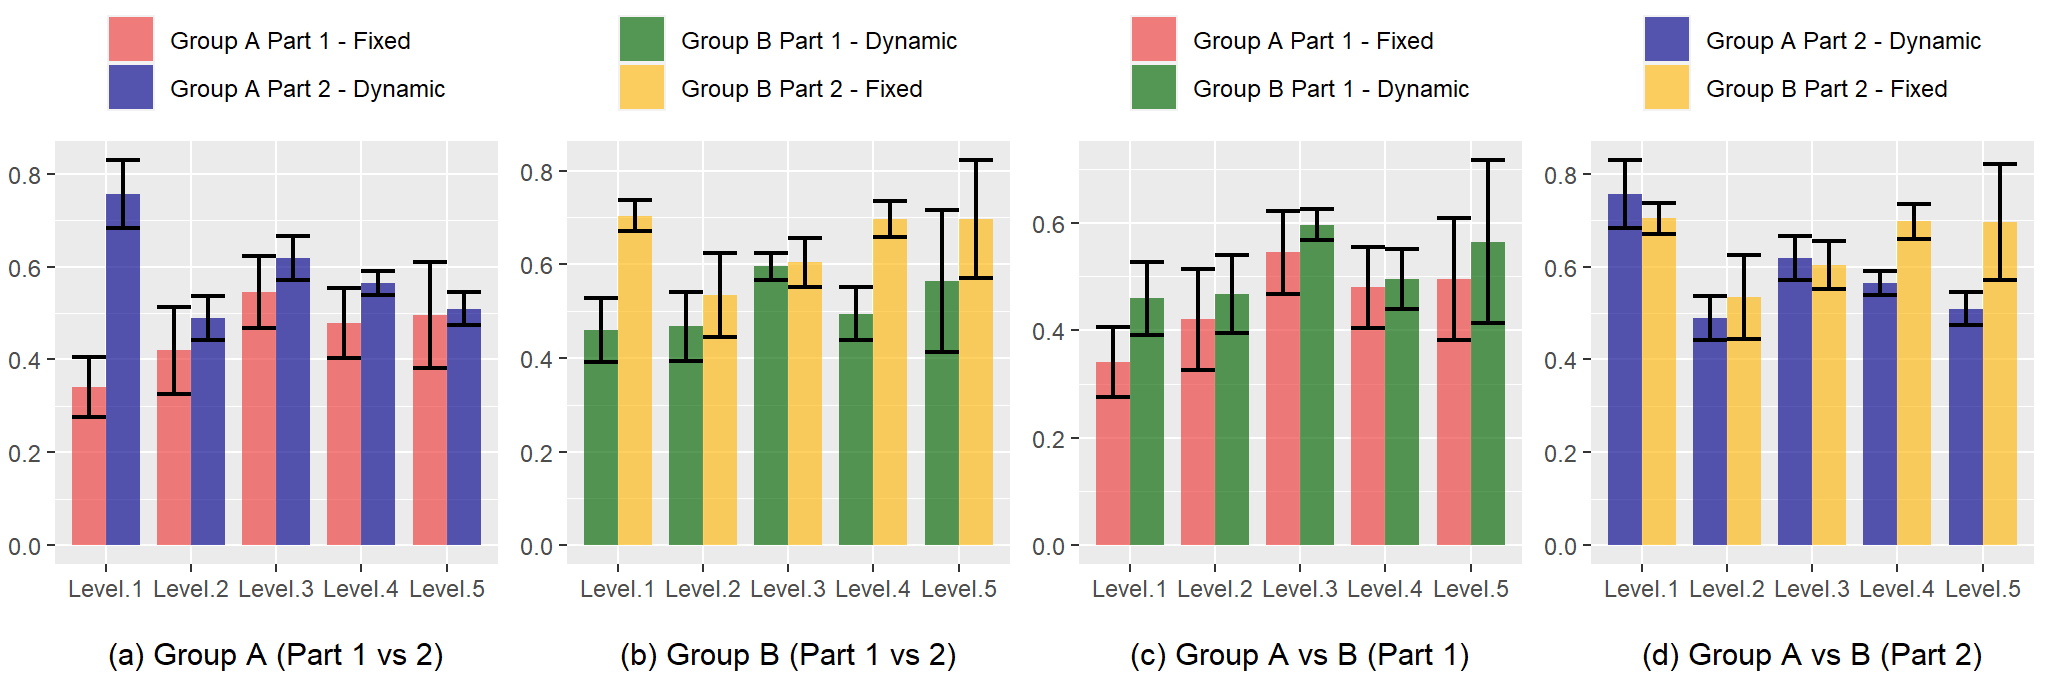
\includegraphics[width=\textwidth]{figures/attack_avoidance_efficiency-intermediate_players.png}
        \legend{Source: Assembled by authors.}
        \label{fig:result-metric-intermediates-attack-avoidance-efficiency}
    \end{center}
\end{figure}

%attack_window_efficiency
% Avg Attack Window Efficiency per Level - Intermediates
% =======================
\begin{figure}[!ht]
    \begin{center}
    \caption{Avg. Attack Window Efficiency (Y) per Level (X) for Intermediates.}
        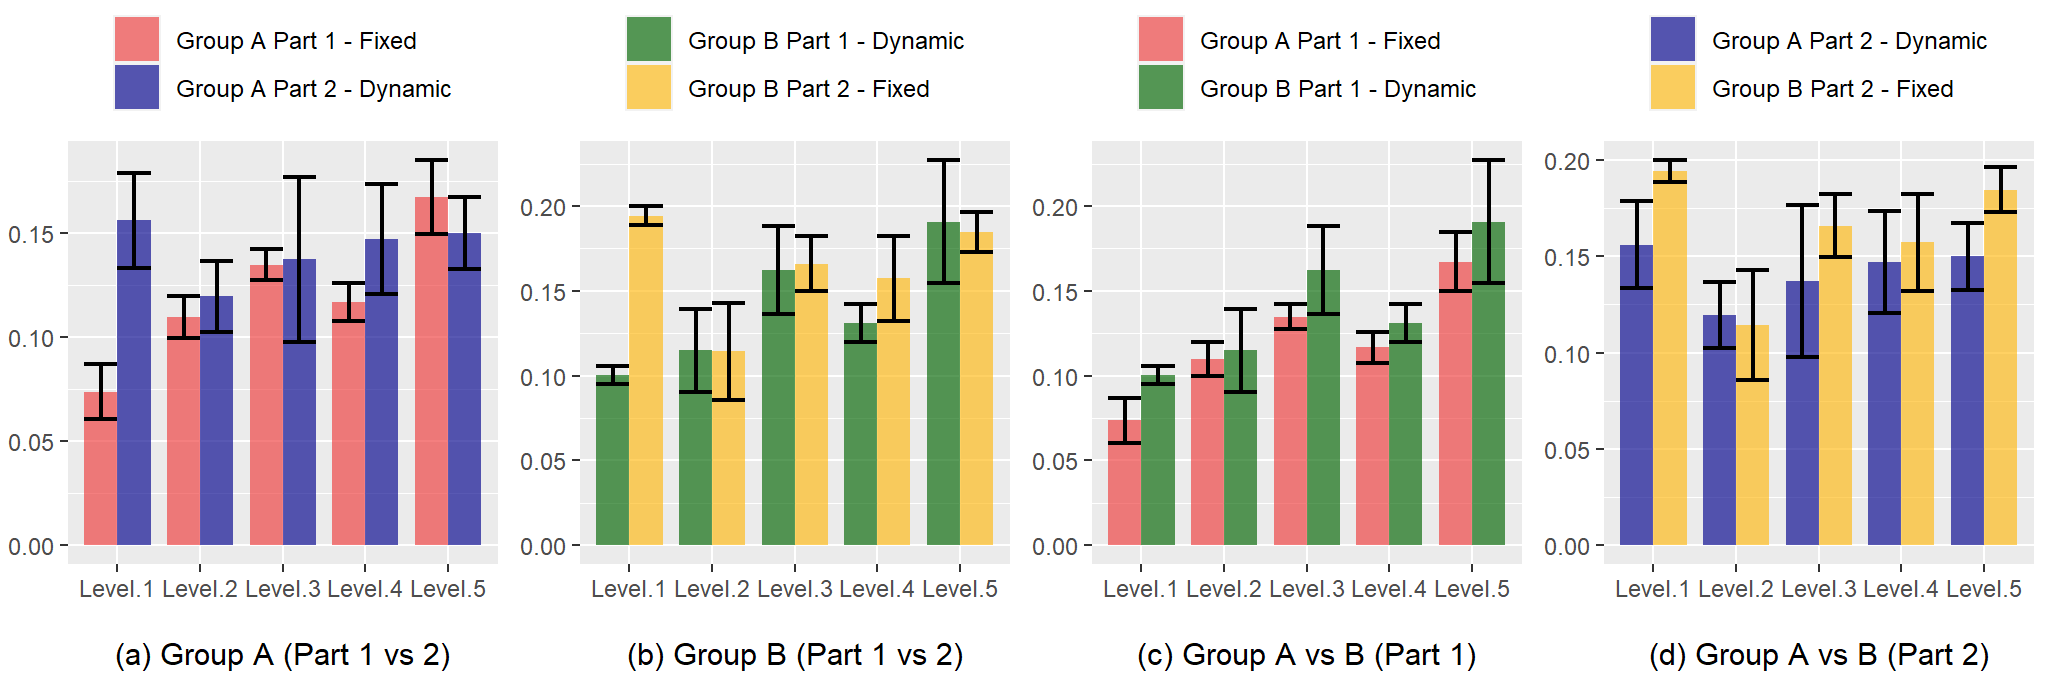
\includegraphics[width=\textwidth]{figures/attack_window_efficiency-intermediate_players.png}
        \legend{Source: Assembled by authors.}
        \label{fig:result-metric-intermediates-attack-window-efficiency}
    \end{center}
\end{figure}

%completion_time
% Avg Completion Time per Level - Intermediates
% =======================
\begin{figure}[!ht]
    \begin{center}
    \caption{Avg. Completion Time (Y) per Level (X) for Intermediates.}
        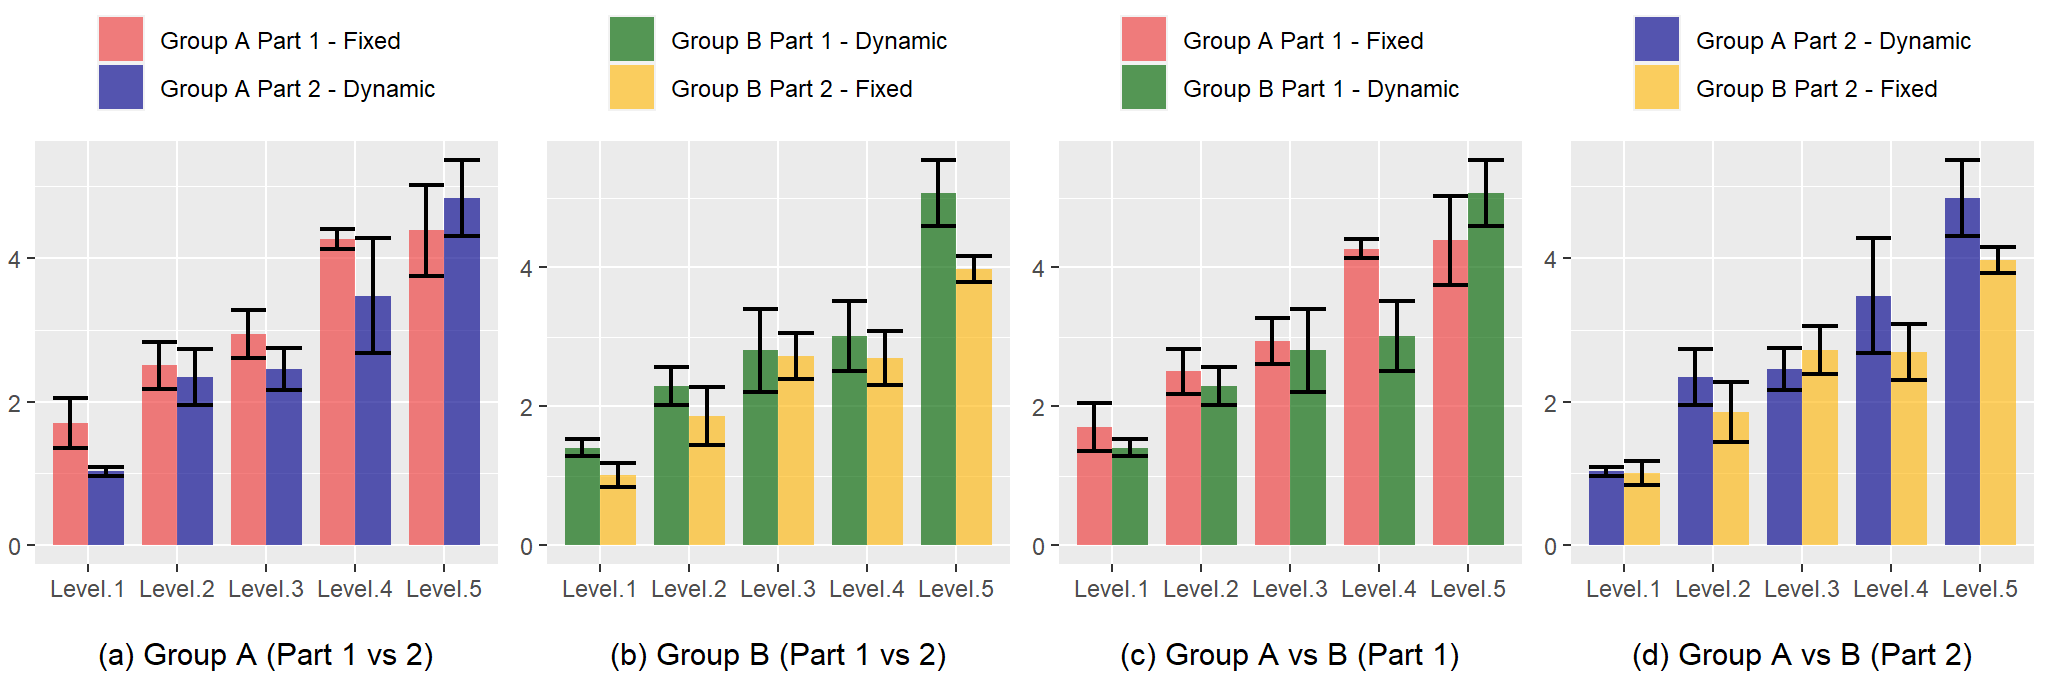
\includegraphics[width=\textwidth]{figures/completion_time-intermediate_players.png}
        \legend{Source: Assembled by authors.}
        \label{fig:result-metric-intermediates-completion-time}
    \end{center}
\end{figure}

%damage_dealt_per_10s
% Avg Damage Dealt per 10s per Level - Intermediates
% =======================
\begin{figure}[!ht]
    \begin{center}
    \caption{Avg. Damage Dealt per 10 seconds (Y) per Level (X) for Intermediates.}
        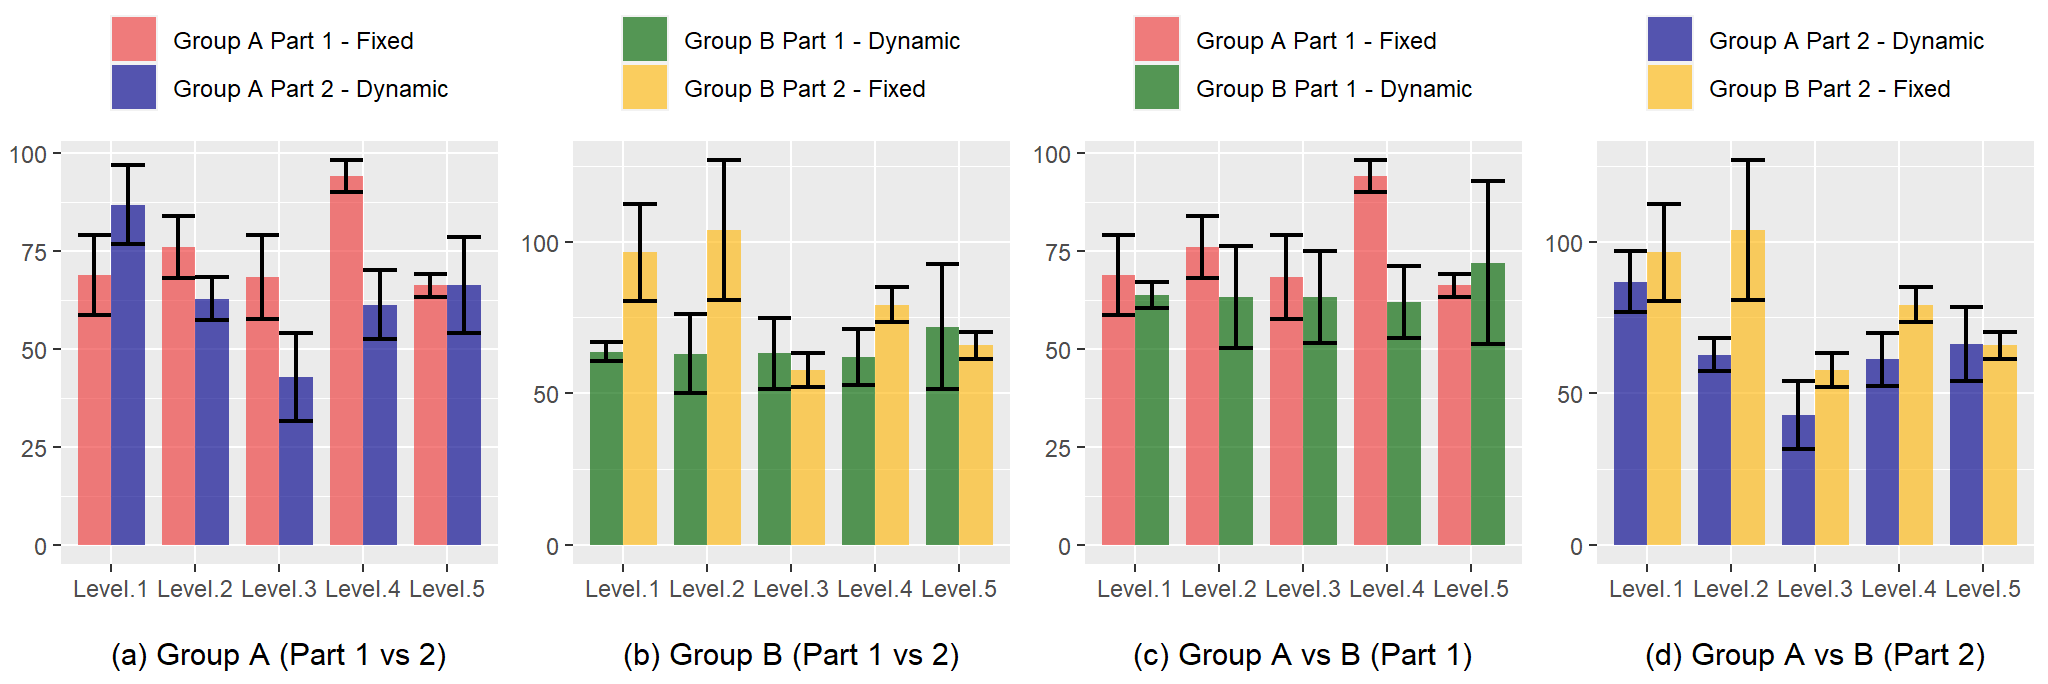
\includegraphics[width=\textwidth]{figures/damage_dealt_per_10s-intermediate_players.png}
        \legend{Source: Assembled by authors.}
        \label{fig:result-metric-intermediates-damage-dealt-per-10s}
    \end{center}
\end{figure}

%deaths_per_level
% Avg Deaths per Level - Intermediates
% =======================
\begin{figure}[!ht]
    \begin{center}
    \caption{Avg. Deaths (Y) per Level (X) for Intermediates.}
        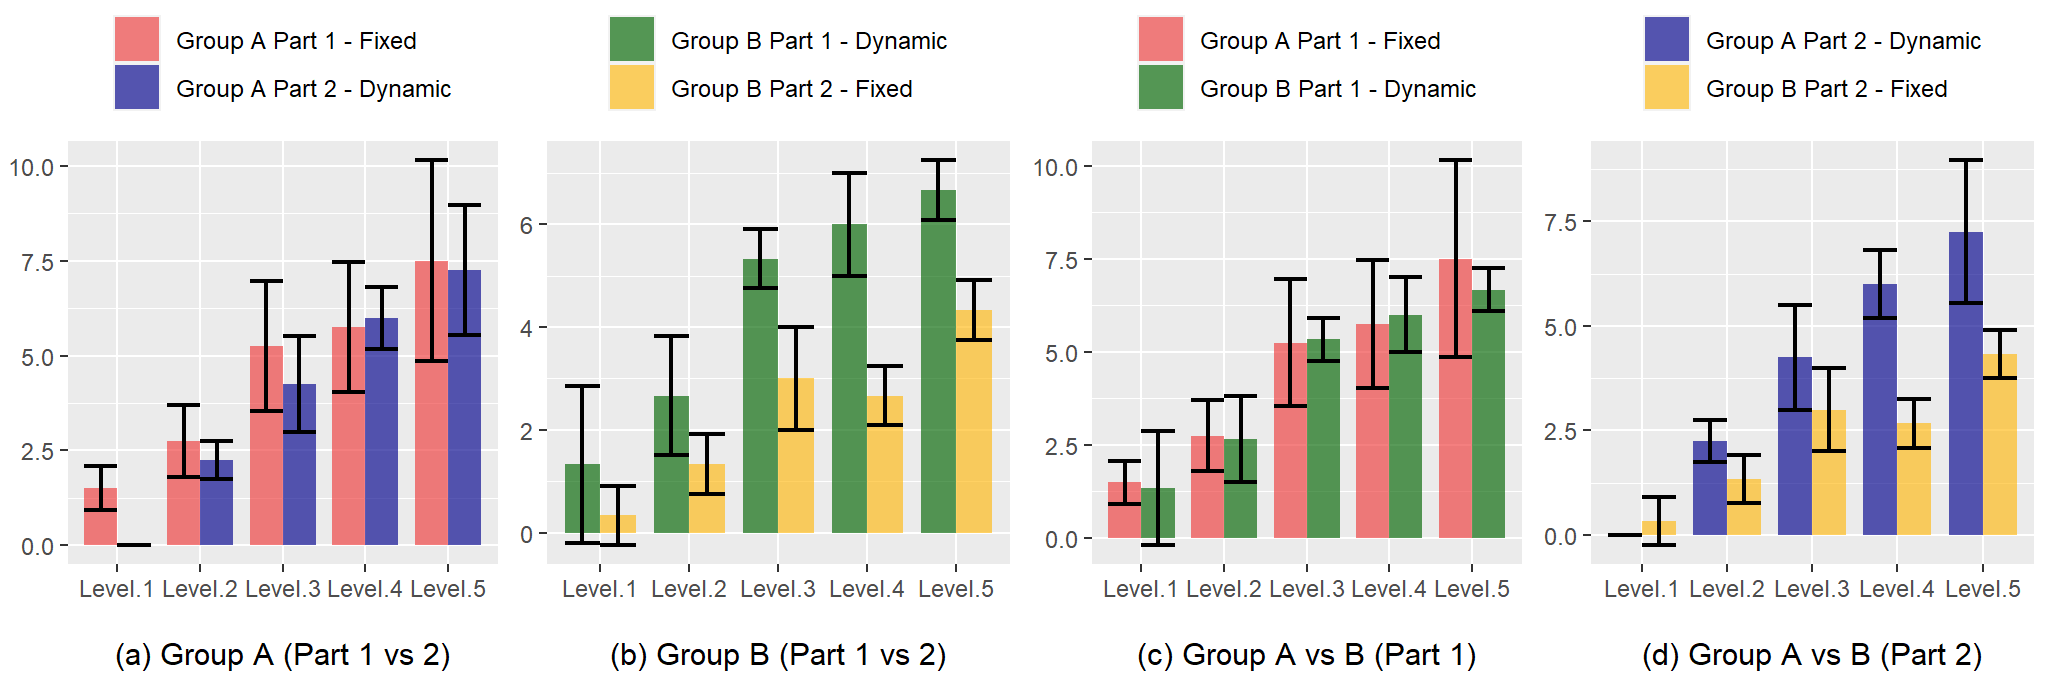
\includegraphics[width=\textwidth]{figures/deaths_per_level-intermediate_players.png}
        \legend{Source: Assembled by authors.}
        \label{fig:result-metric-intermediates-deaths-per-level}
    \end{center}
\end{figure}

%health_lost_per_encounter
% Avg Health Lost per Encounter per Level - Intermediates
% =======================
\begin{figure}[!ht]
    \begin{center}
    \caption{Avg. Health Lost per Encounter (Y) per Level (X) for Intermediates.}
        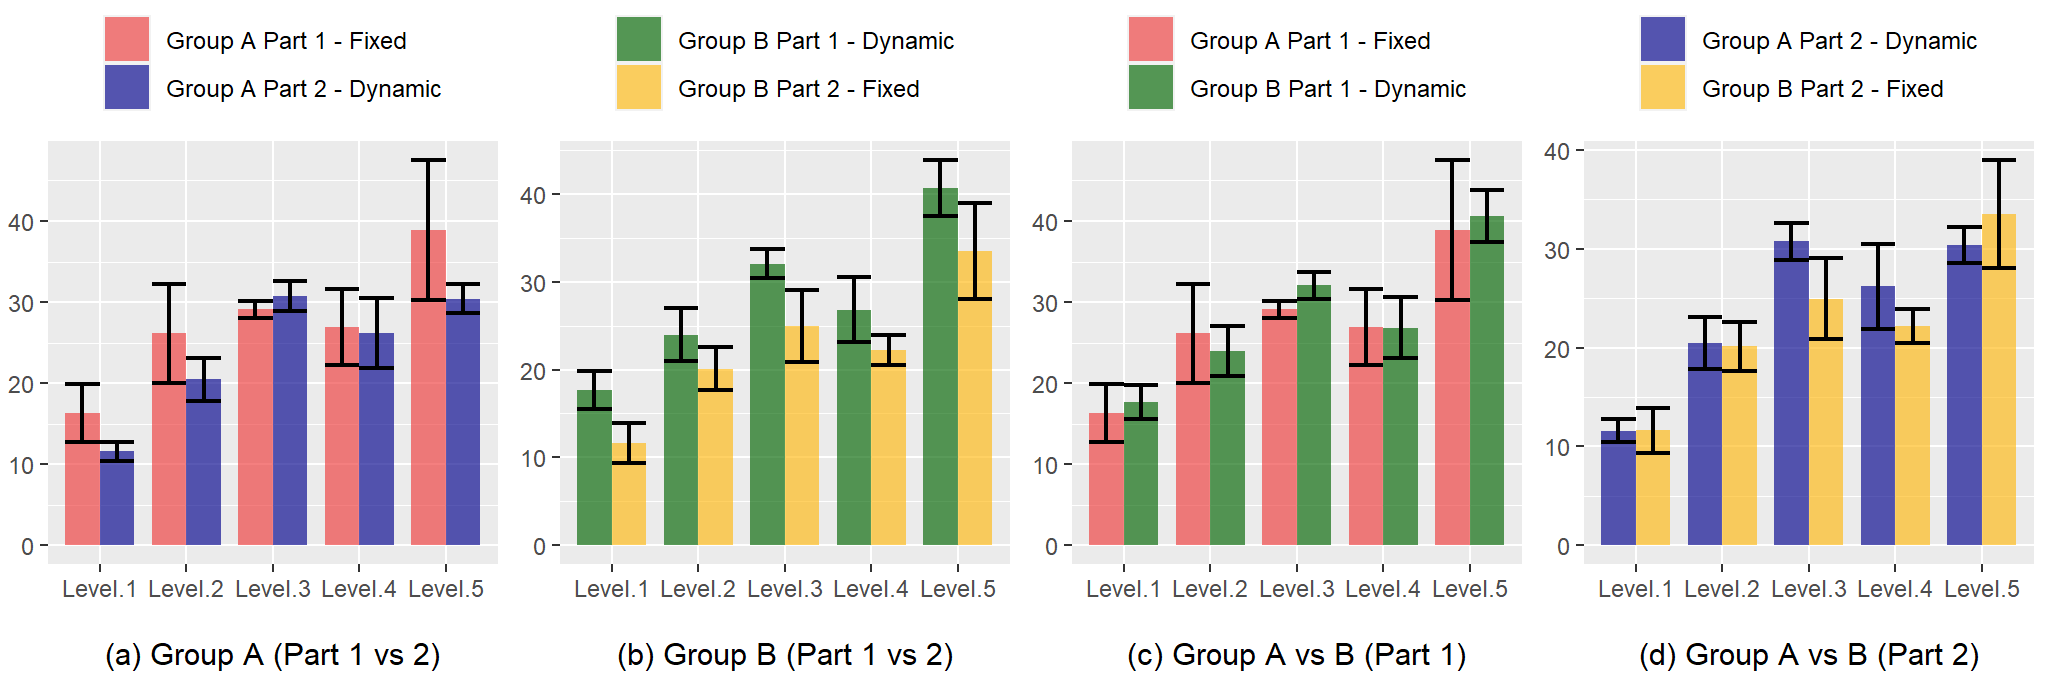
\includegraphics[width=\textwidth]{figures/health_lost_per_encounter-intermediate_players.png}
        \legend{Source: Assembled by authors.}
        \label{fig:result-metric-intermediates-health-lost-per-encounter}
    \end{center}
\end{figure}

% Perception
% =============================

% TODO write paragraphs

% Perceptions on Difficulty -- Intermediate Players
% =======================
\begin{figure}[!ht]
    \begin{center}
    \caption{Perceptions on Difficulty - Intermediate Players.}
        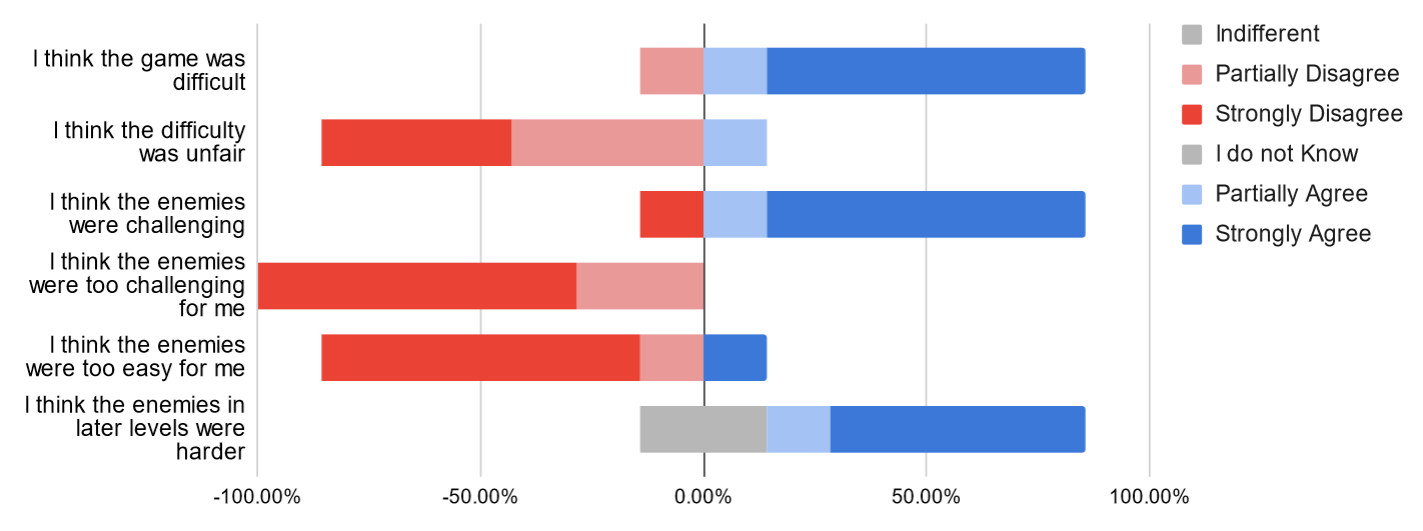
\includegraphics[width=36em]{figures/fig-perception-difficulty-intermediate-players.png}
        \legend{Source: Chart assembled by authors.}
        \label{fig:perception-difficulty-intermediate-players}
    \end{center}
\end{figure}

% Perceptions on Learning -- Intermediate Players
% =======================
\begin{figure}[!ht]
    \begin{center}
    \caption{Perceptions on Learning - Intermediate Players.}
        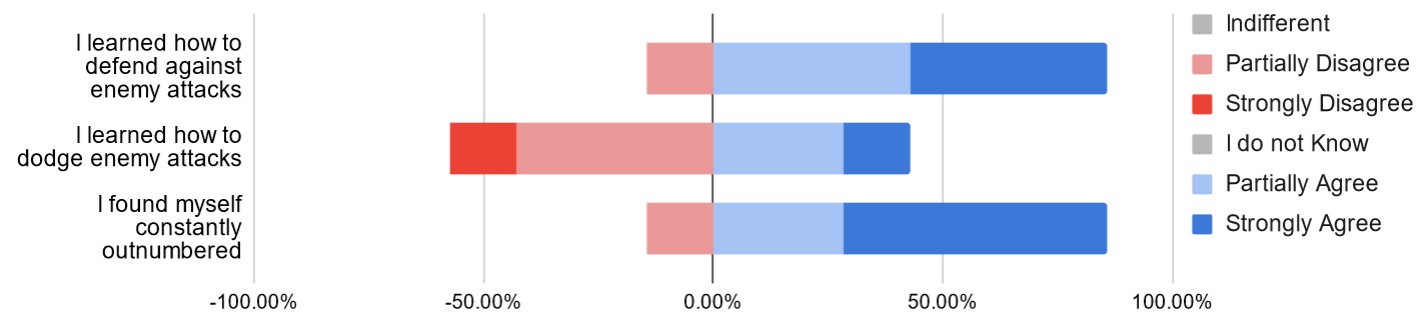
\includegraphics[width=36em]{figures/fig-perception-learning-intermediate-players.png}
        \legend{Source: Chart assembled by authors.}
        \label{fig:perception-learning-intermediate-players}
    \end{center}
\end{figure}

% Perceptions on Playthroughs -- Intermediate Players Group A
% =======================
\begin{figure}[!ht]
    \begin{center}
    \caption{Perceptions on Playthroughs - Intermediate Players Group A.}
        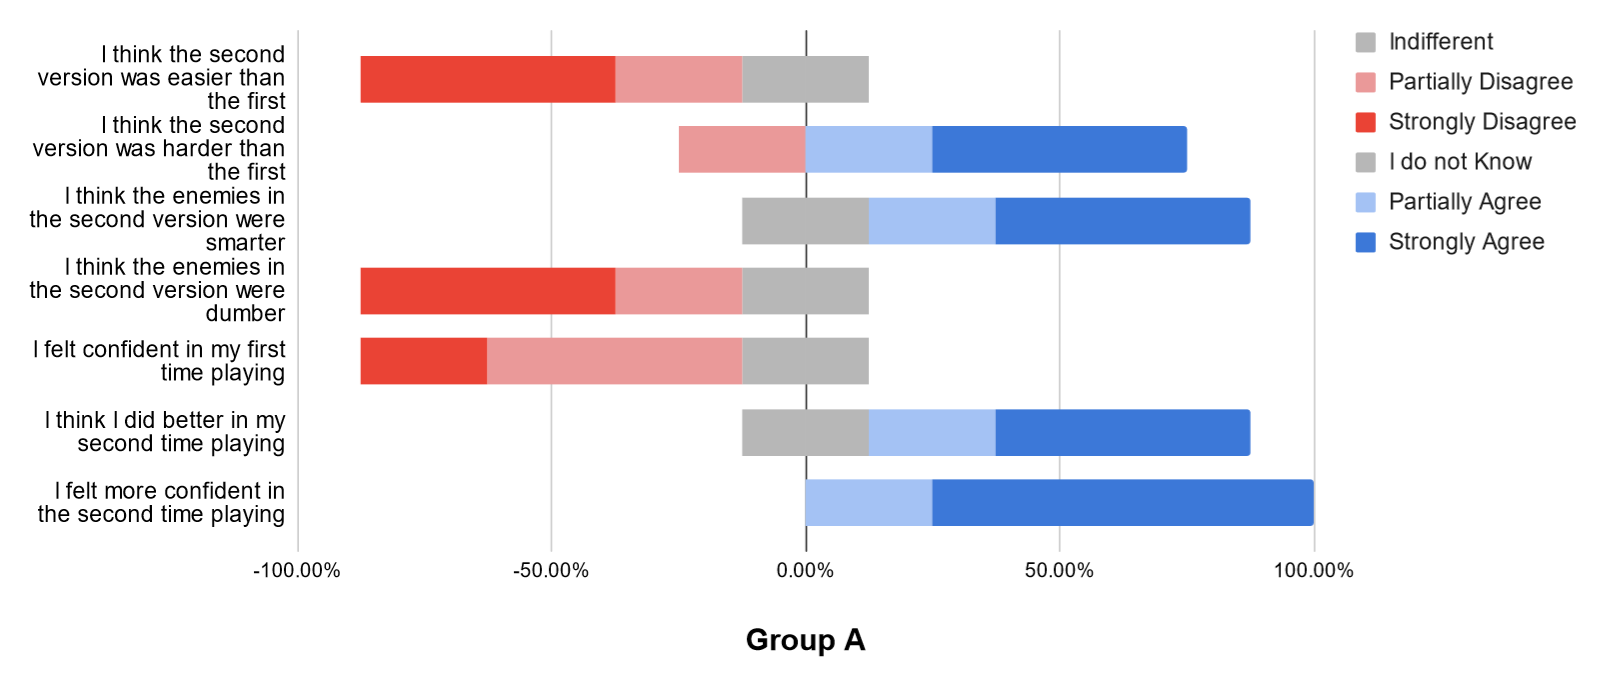
\includegraphics[width=36em]{figures/fig-perception-versions-intermediate-players-group-a.png}
        \legend{Source: Chart assembled by authors.}
        \label{fig:perception-playthrough-intermediate-players-group-a}
    \end{center}
\end{figure}

% Perceptions on Playthroughs -- Intermediate Players Group B
% =======================
\begin{figure}[!ht]
    \begin{center}
    \caption{Perceptions on Playthroughs - Intermediate Players Group B.}
        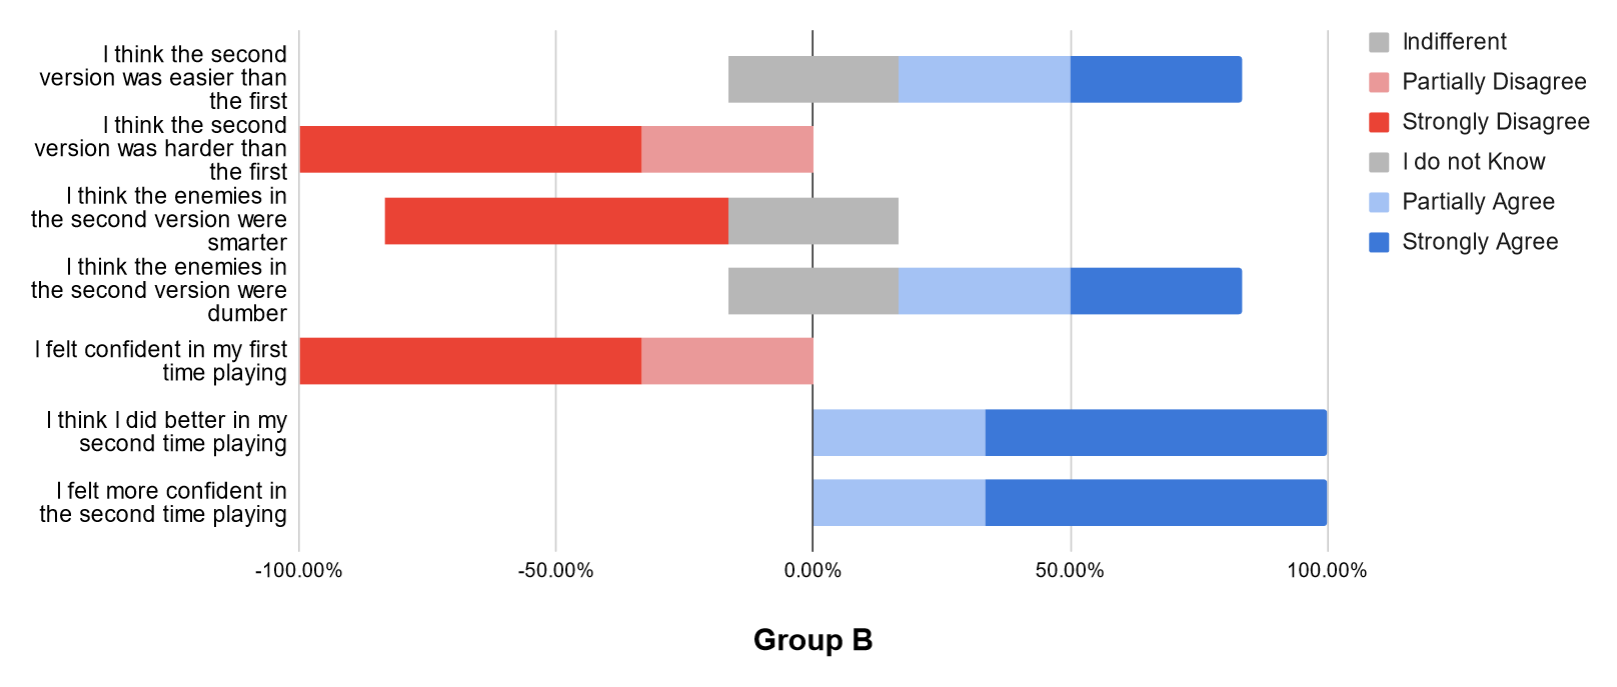
\includegraphics[width=36em]{figures/fig-perception-versions-intermediate-players-group-b.png}
        \legend{Source: Chart assembled by authors.}
        \label{fig:perception-playthrough-intermediate-players-group-b}
    \end{center}
\end{figure}

% ==================================================
% ==================================================
% ==================================================

\subsection{Veteran Players}

% TODO write paragraphs

% Performance
% =============================

% Table with Observations for Performance Metrics for Veteran Players
\begin{table}
    \begin{center}
      \caption{Summarized observations on Performance Metrics for Veteran Players.}
      \label{tab:observations-performance-metrics-veterans}
      \rowcolors{2}{}{gray!25} % Alternate row colors
      \begin{tabular}{ >{\small}w{c}{6em} >{\footnotesize}w{l}{25em} } % alignments and column size
        \addlinespace
        \toprule
        % Headings
        \bf Metric & \bf Observations  \\
        \midrule
        % Data
        % ----------------------------------------------------------------
        \makecell[c]{Adjustment\\Targets\\Average} & 
        \makecell*[{{p{30em}}}]
        {
            \textbullet\space Observation 1. \\
            \textbullet\space Observation 2. \\
            \textbullet\space Observation 3. \\
        } \\
        % ----------------------------------------------------------------
        % Attack avoidance efficiency
        \makecell[c]{Attack\\Avoidance\\Efficiency} & 
        \makecell*[{{p{30em}}}]
        {
            \textbullet\space Observation 1. \\
            \textbullet\space Observation 2. \\
            \textbullet\space Observation 3. \\
        } \\
        % ----------------------------------------------------------------
        % Attack Window Efficiency
        \makecell[c]{Attack\\Window\\Efficiency} & 
        \makecell*[{{p{30em}}}]
        {
            \textbullet\space Observation 1. \\
            \textbullet\space Observation 2. \\
            \textbullet\space Observation 3. \\
        } \\
        % ----------------------------------------------------------------
        % Completion time
        \makecell[c]{Completion\\Time} & 
        \makecell*[{{p{30em}}}]
        {
            \textbullet\space Observation 1. \\
            \textbullet\space Observation 2. \\
            \textbullet\space Observation 3. \\
        } \\
        % ----------------------------------------------------------------
        % Damage Dealth per 10 seconds
        \makecell[c]{Damage Dealt\\per 10 seconds} & 
        \makecell*[{{p{30em}}}]
        {
            \textbullet\space Observation 1. \\
            \textbullet\space Observation 2. \\
            \textbullet\space Observation 3. \\
        } \\
        % ----------------------------------------------------------------
        % Deaths per Level
        \makecell[c]{Deaths per\\Level} & 
        \makecell*[{{p{30em}}}]
        {
            \textbullet\space Observation 1. \\
            \textbullet\space Observation 2. \\
            \textbullet\space Observation 3. \\
        } \\
        % ----------------------------------------------------------------
        % Health Lost per Encounter
        \makecell[c]{Health Lost\\per Encounter} & 
        \makecell*[{{p{30em}}}]
        {
            \textbullet\space Observation 1. \\
            \textbullet\space Observation 2. \\
            \textbullet\space Observation 3. \\
        } \\
        % ----------------------------------------------------------------  
        \bottomrule
      \end{tabular}
    \end{center}
\end{table}

%adjustment_target_level
% Avg Adjustment Target per Level - Veterans
% =======================
\begin{figure}[!ht]
    \begin{center}
    \caption{Avg. Adjustment Targets Average (Y) per Level (X) for Veterans.}
        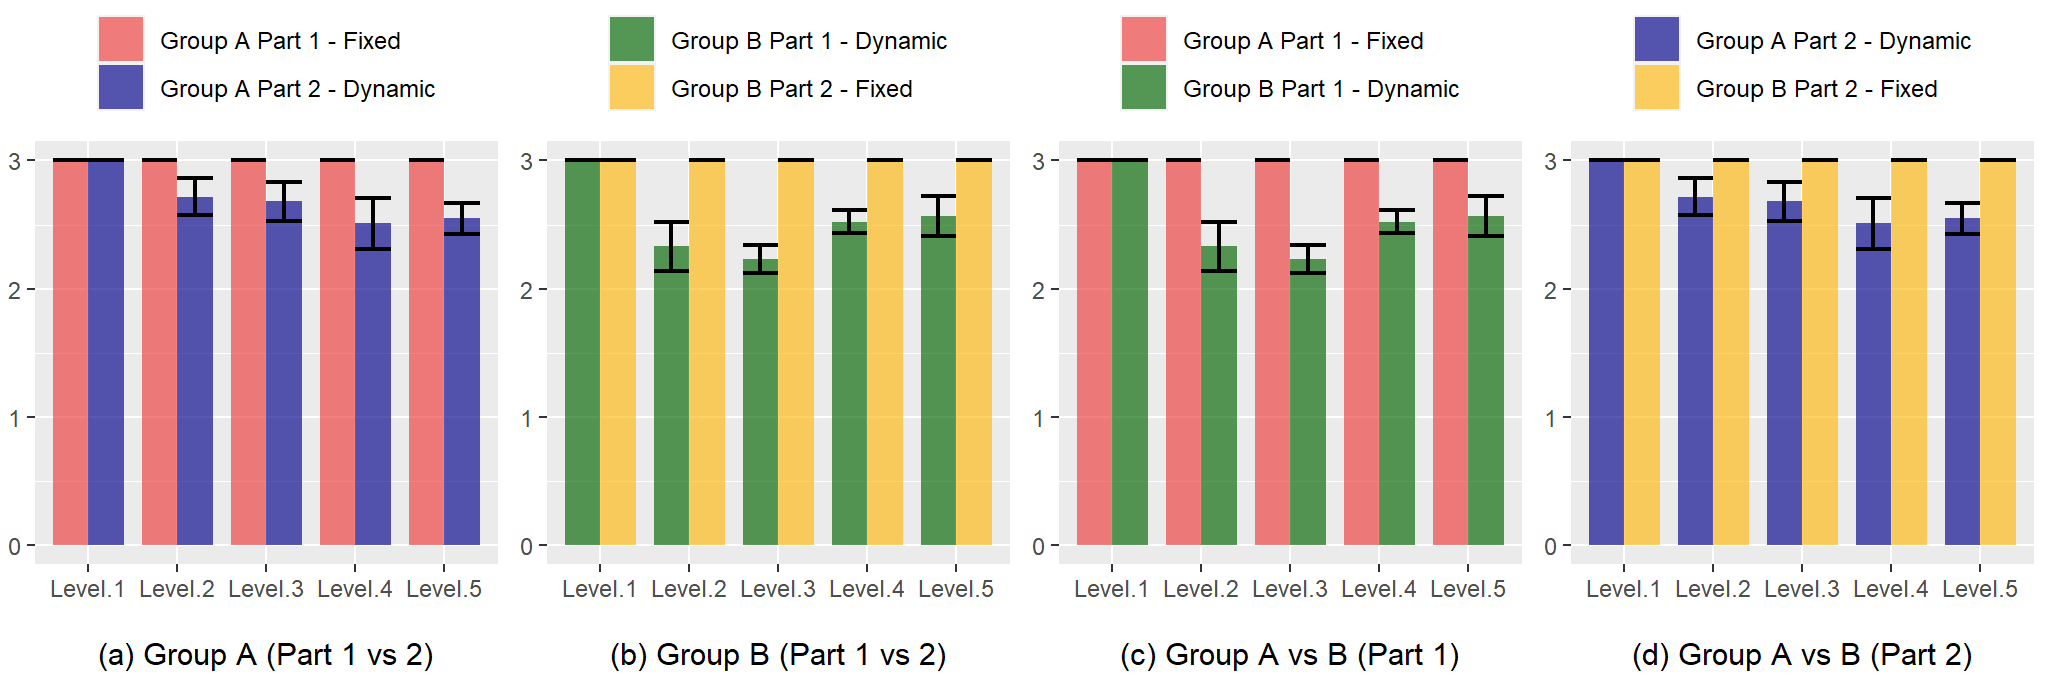
\includegraphics[width=\textwidth]{figures/adjustment_target_level-veteran_players.png}
    \legend{Source: Assembled by authors.}
    \label{fig:result-metric-veteran-adjustment-target-level}
    \end{center}
\end{figure}

%attack_avoidance_efficiency
% Avg Attack Avoidance Efficiency per Level - Veterans
% =======================
\begin{figure}[!ht]
    \begin{center}
        \caption{Avg. Attack Avoidance Efficiency (Y) per Level (X) for Veterans.}
        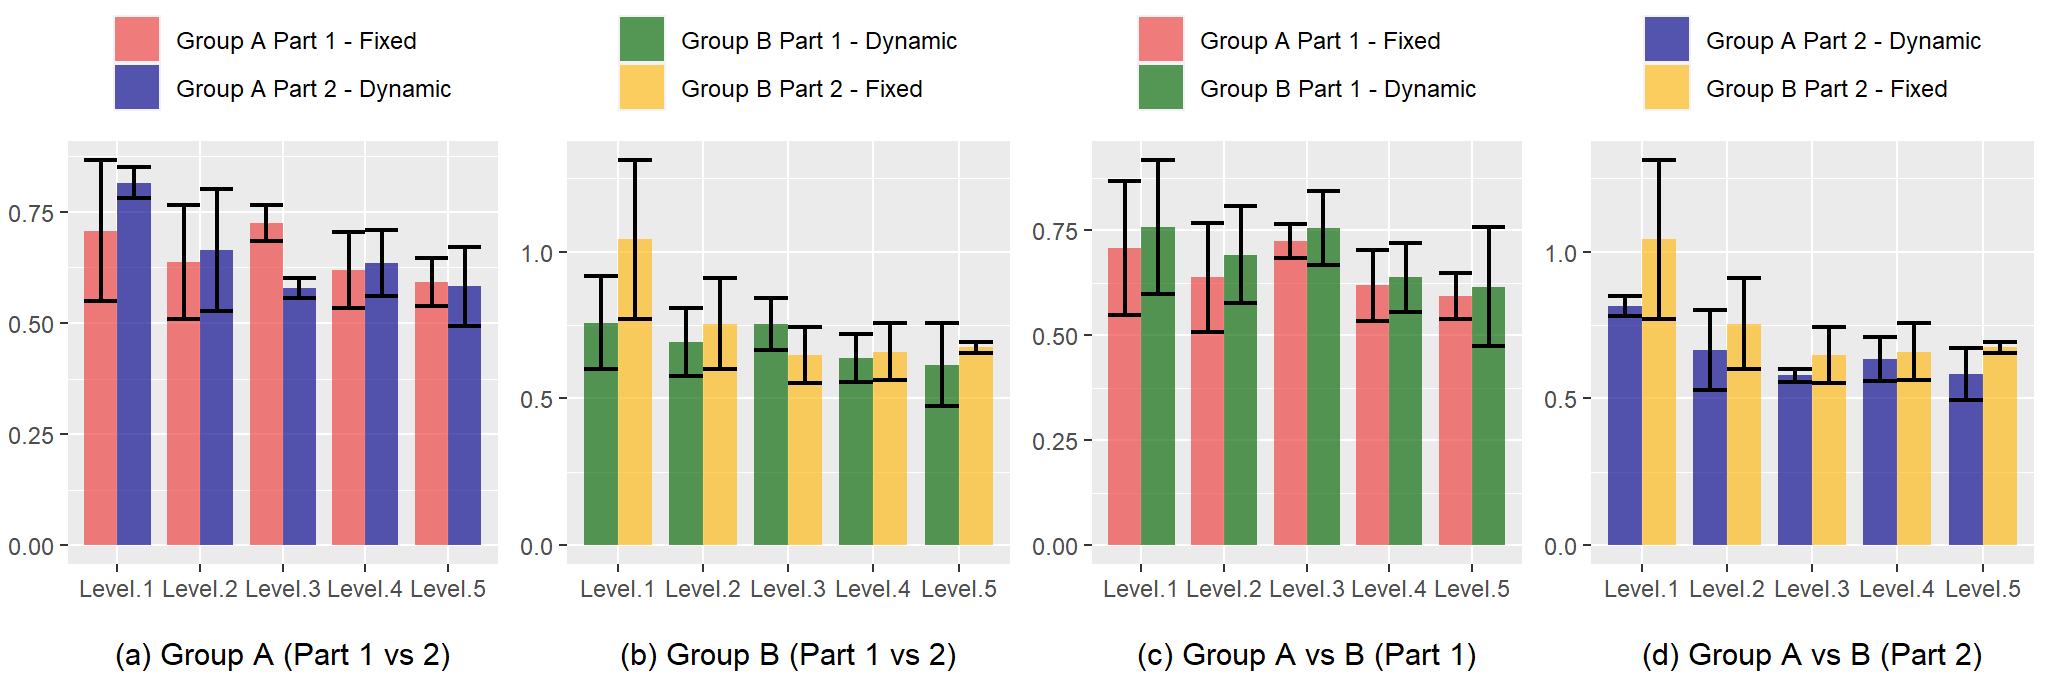
\includegraphics[width=\textwidth]{figures/attack_avoidance_efficiency-veteran_players.png}
    \legend{Source: Assembled by authors.}
    \label{fig:result-metric-veterans-attack-avoidance-efficiency}
    \end{center}
\end{figure}

%attack_window_efficiency
% Avg Attack Window Efficiency per Level - Veterans
% =======================
\begin{figure}[!ht]
    \begin{center}
    \caption{Avg. Attack Window Efficiency (Y) per Level (X) for Veterans.}
        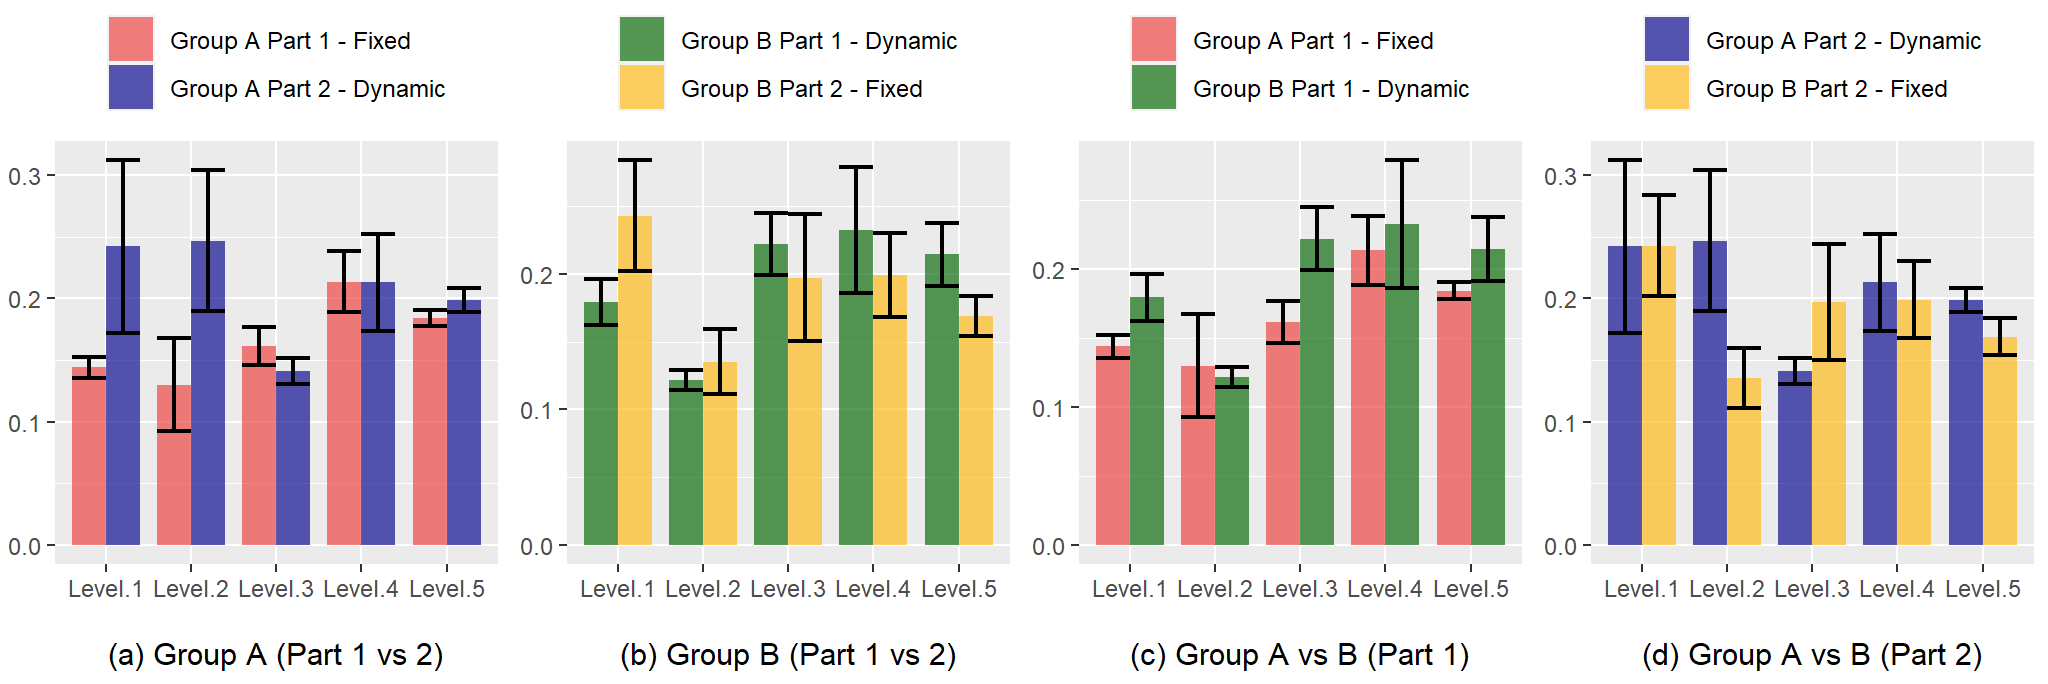
\includegraphics[width=\textwidth]{figures/attack_window_efficiency-veteran_players.png}
    \legend{Source: Assembled by authors.}
    \label{fig:result-metric-veterans-attack-window-efficiency}
    \end{center}
\end{figure}

%completion_time
% Avg Completion Time per Level - Veterans
% =======================
\begin{figure}[!ht]
    \begin{center}
    \caption{Avg. Completion Time (Y) per Level (X) for Veterans.}
        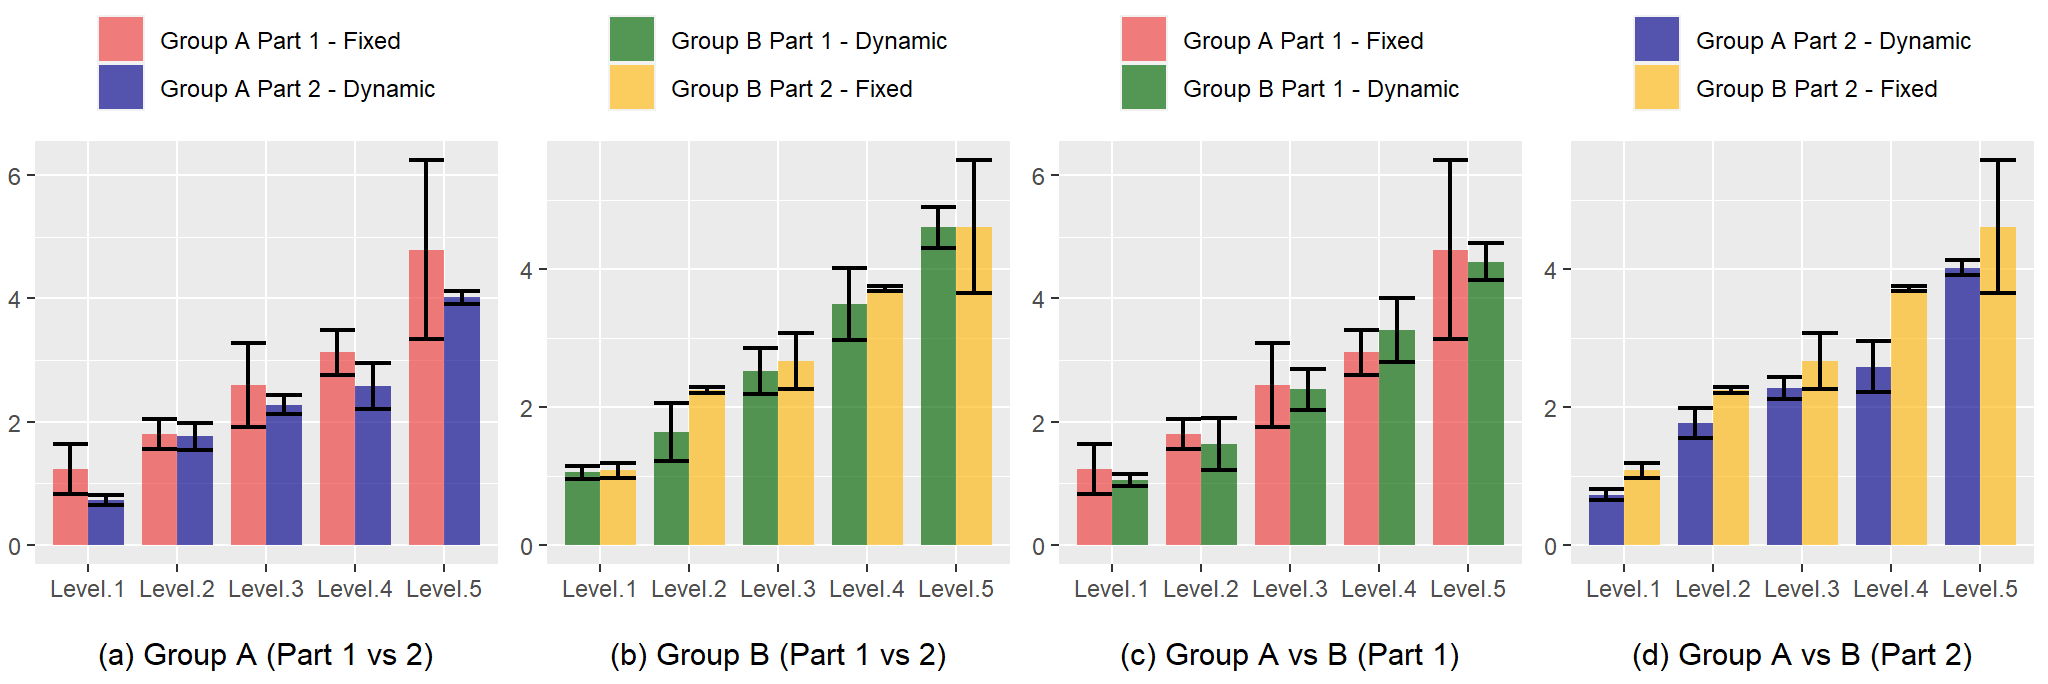
\includegraphics[width=\textwidth]{figures/completion_time-veteran_players.png}
        \legend{Source: Assembled by authors.}
        \label{fig:result-metric-veterans-completion-time}
    \end{center}
\end{figure}

%damage_dealt_per_10s
% Avg Damage Dealt per 10s per Level - Veterans
% =======================
\begin{figure}[!ht]
    \begin{center}
    \caption{Avg. Damage Dealt per 10 seconds (Y) per Level (X) for Veterans.}
        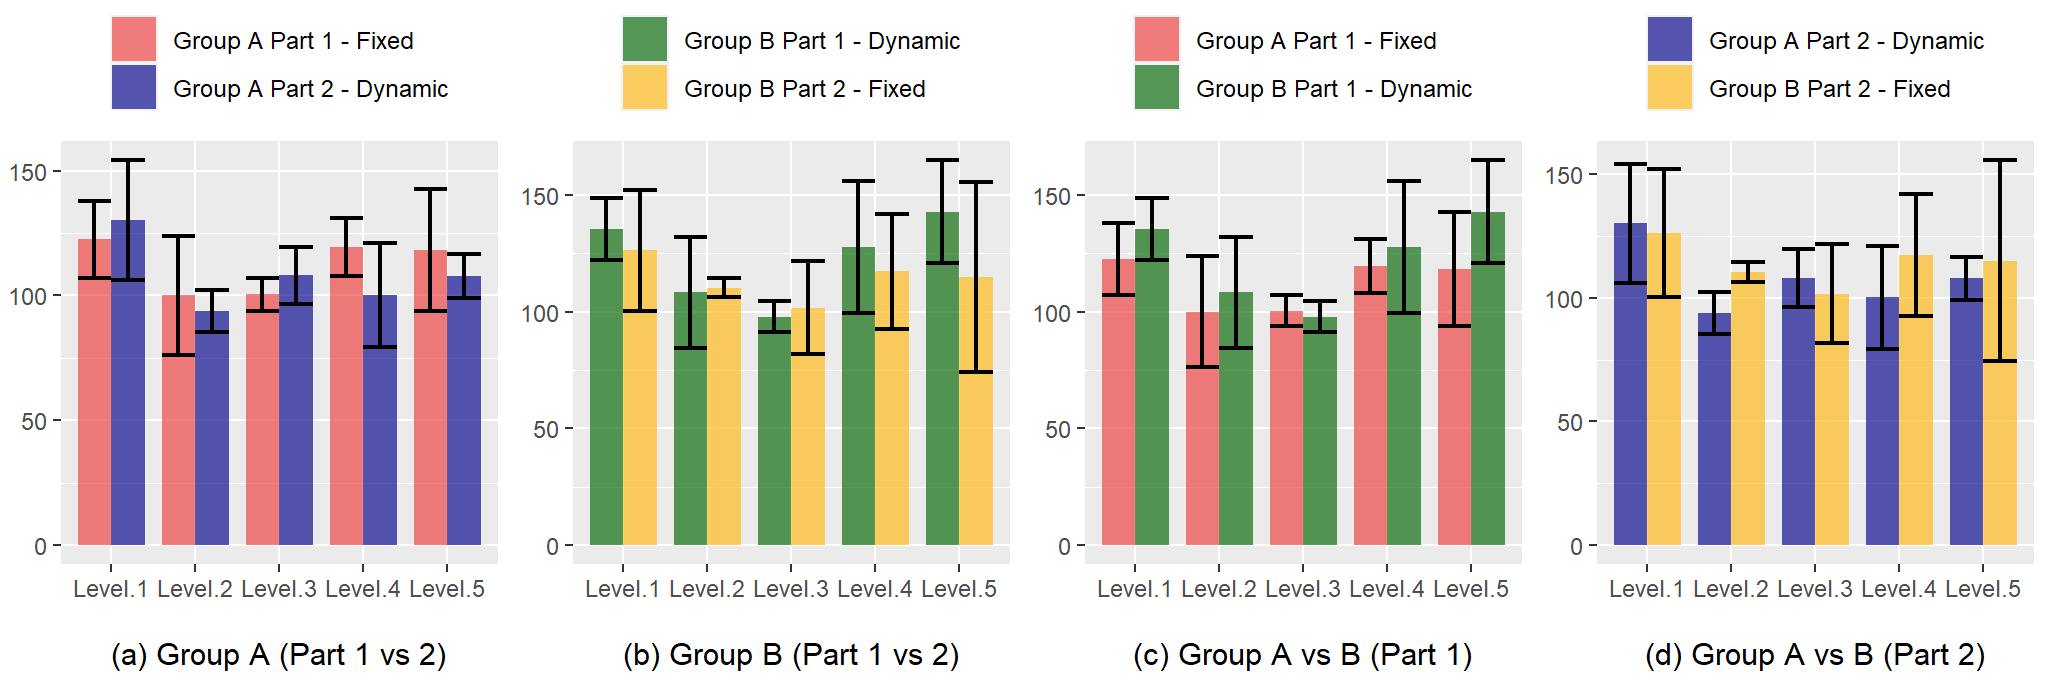
\includegraphics[width=\textwidth]{figures/damage_dealt_per_10s-veteran_players.png}
        \legend{Source: Assembled by authors.}
        \label{fig:result-metric-veterans-damage-dealt-per-10s}
    \end{center}
\end{figure}

%deaths_per_level
% Avg Deaths per Level - Veterans
% =======================
\begin{figure}[!ht]
    \begin{center}
    \caption{Avg. Deaths (Y) per Level (X) for Veterans.}
        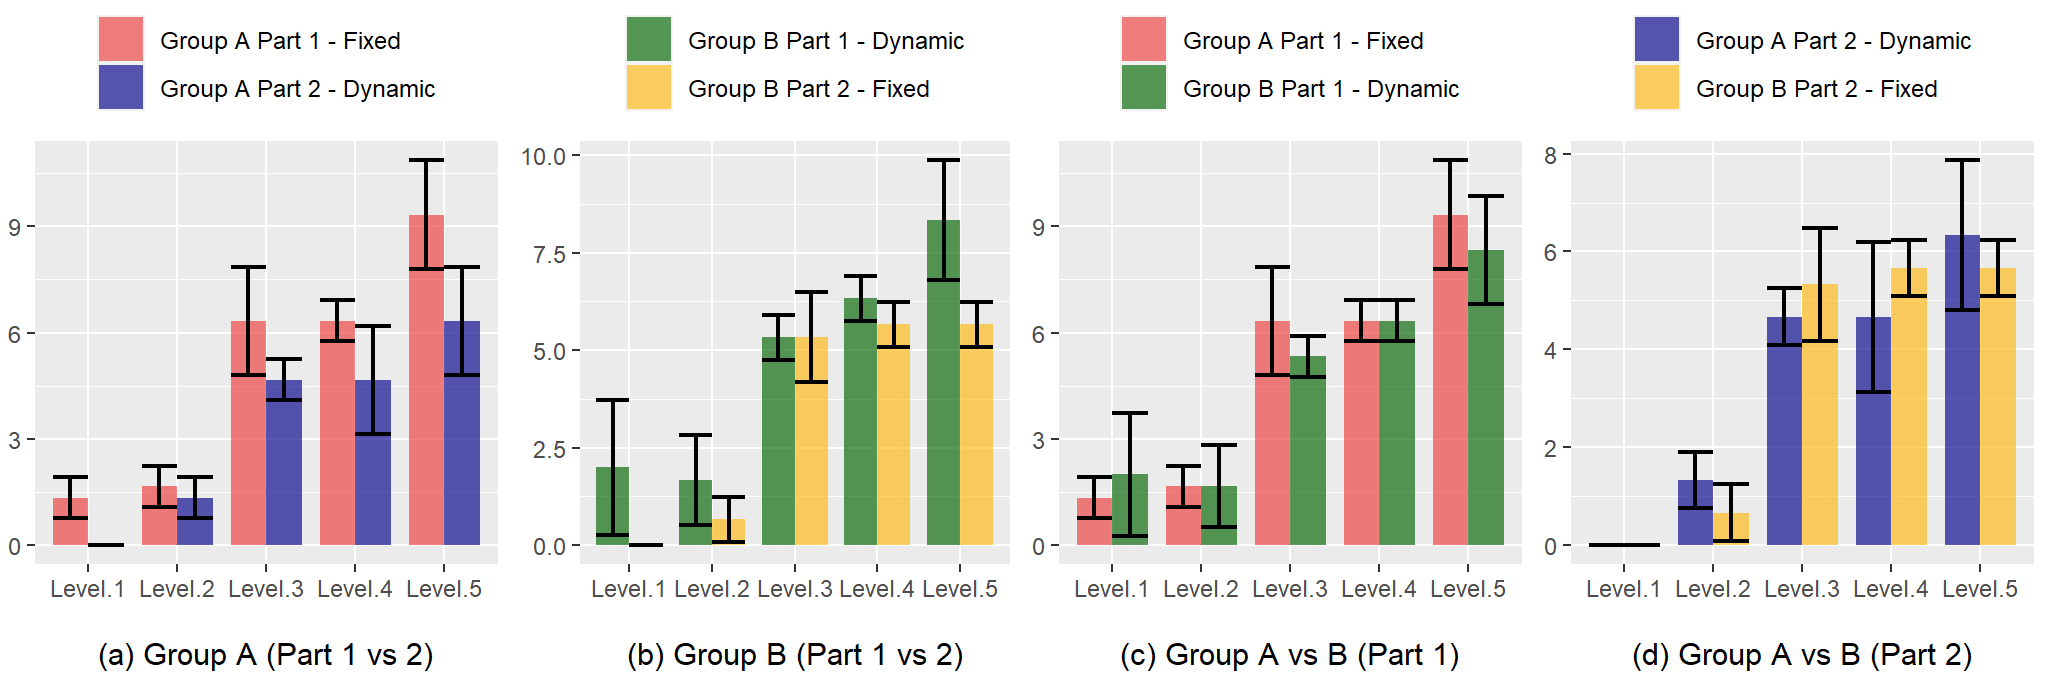
\includegraphics[width=\textwidth]{figures/deaths_per_level-veteran_players.png}
        \legend{Source: Assembled by authors.}
        \label{fig:result-metric-veterans-deaths-per-level}
    \end{center}
\end{figure}

%health_lost_per_encounter
% Avg Health Lost per Encounter per Level - Veterans
% =======================
\begin{figure}[!ht]
    \begin{center}
    \caption{Avg. Health Lost per Encounter (Y) per Level (X) for Veterans.}
        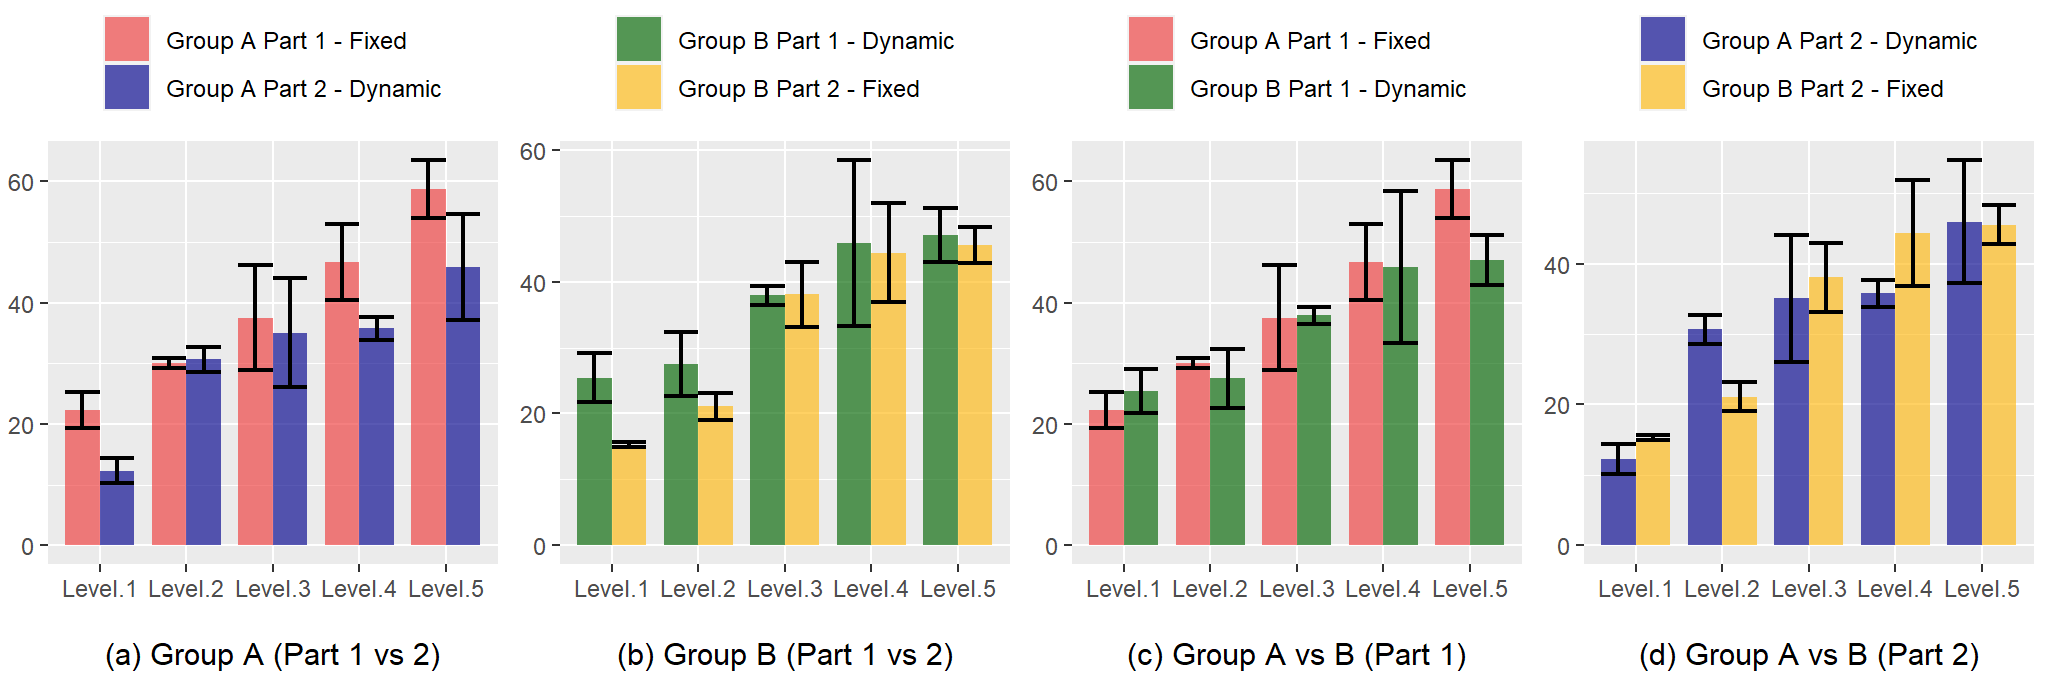
\includegraphics[width=\textwidth]{figures/health_lost_per_encounter-veteran_players.png}
        \legend{Source: Assembled by authors.}
        \label{fig:result-metric-veterans-health-lost-per-encounter}
    \end{center}
\end{figure}

% Perception
% =============================

% TODO write paragraphs

% Perceptions on Difficulty -- Veteran Players
% =======================
\begin{figure}[!ht]
    \begin{center}
    \caption{Perceptions on Difficulty - Veteran Players.}
        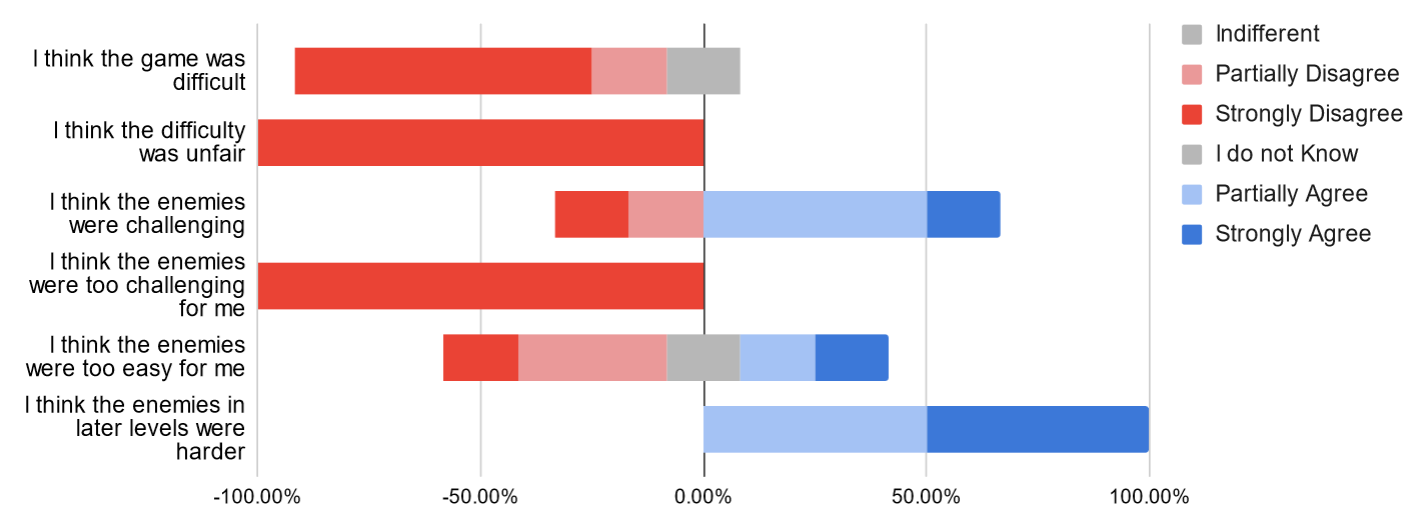
\includegraphics[width=36em]{figures/fig-perception-difficulty-veteran-players.png}
        \legend{Source: Chart assembled by authors.}
        \label{fig:perception-difficulty-veteran-players}
    \end{center}
\end{figure}

% Perceptions on Learning -- Veteran Players
% =======================
\begin{figure}[!ht]
    \begin{center}
    \caption{Perceptions on Learning - Veteran Players.}
        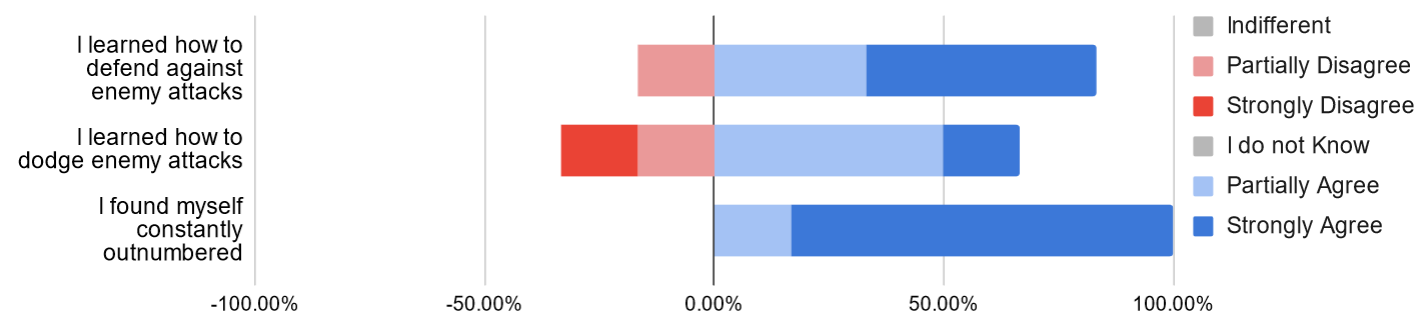
\includegraphics[width=36em]{figures/fig-perception-learning-veteran-players.png}
        \legend{Source: Chart assembled by authors.}
        \label{fig:perception-learning-veteran-players}
    \end{center}
\end{figure}

% Perceptions on Playthroughs -- Veteran Players Group A
% =======================
\begin{figure}[!ht]
    \begin{center}
    \caption{Perceptions on Playthroughs - Veteran Players Group A.}
        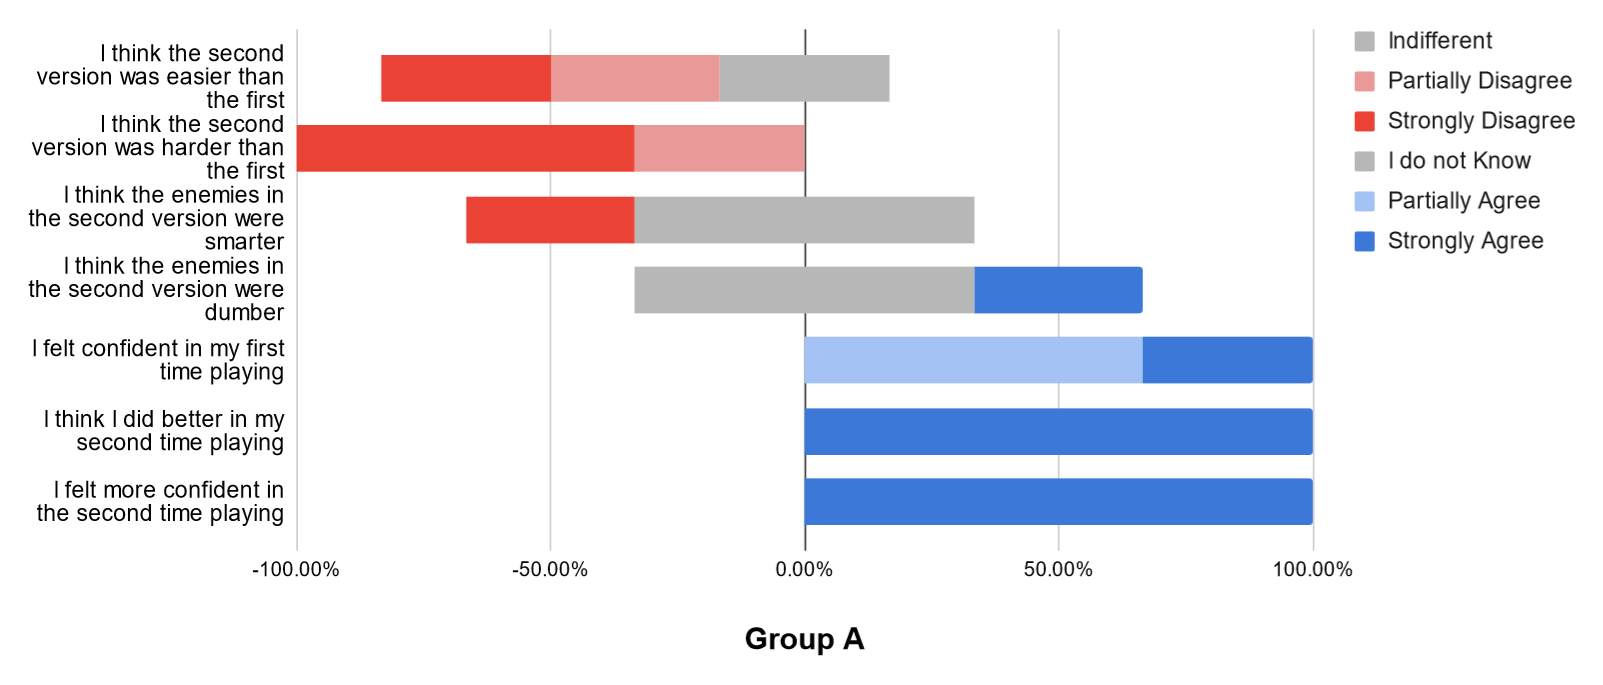
\includegraphics[width=36em]{figures/fig-perception-versions-veteran-players-group-a.png}
        \legend{Source: Chart assembled by authors.}
        \label{fig:perception-playthrough-veteran-players-group-a}
    \end{center}
\end{figure}

% Perceptions on Playthroughs -- Veteran Players Group B
% =======================
\begin{figure}[!ht]
    \begin{center}
    \caption{Perceptions on Playthroughs - Veteran Players Group B.}
        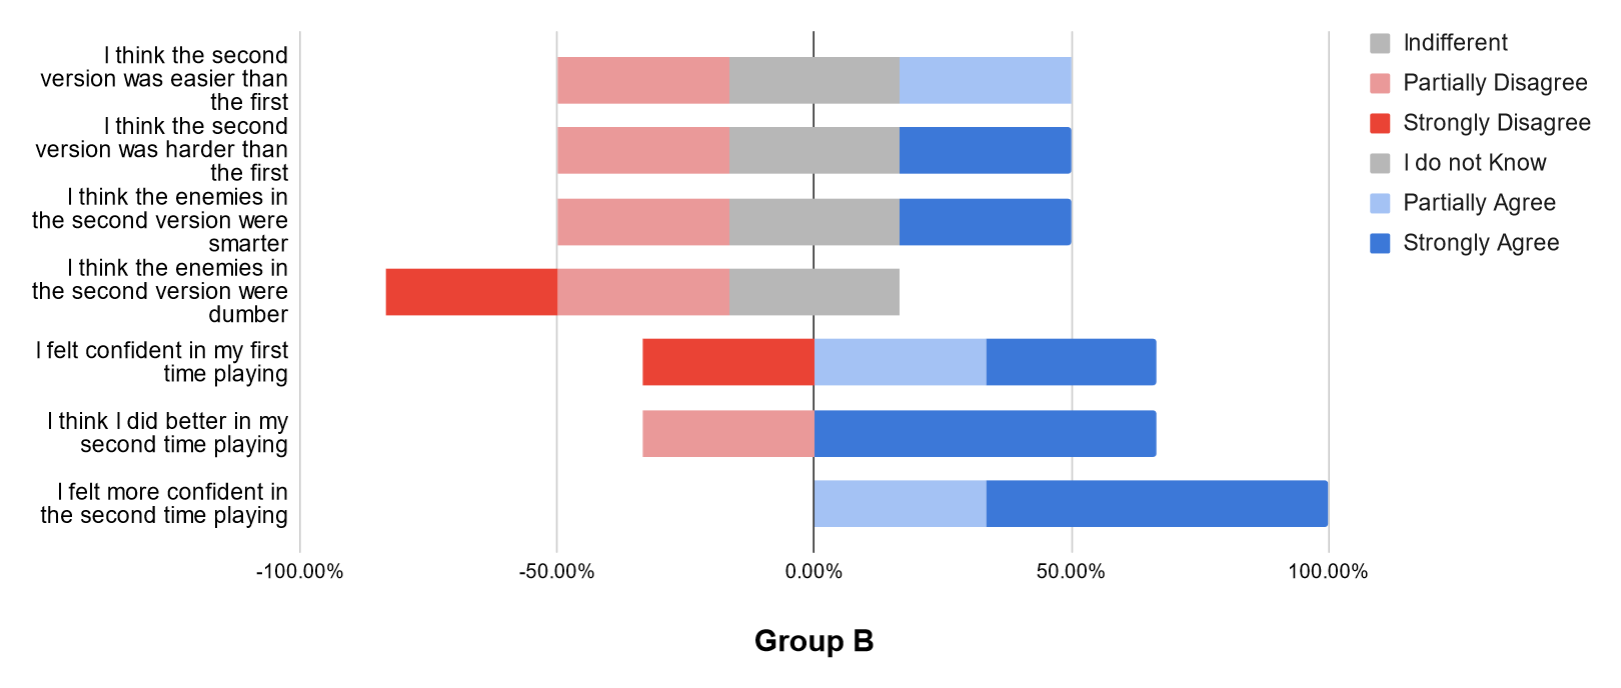
\includegraphics[width=36em]{figures/fig-perception-versions-veteran-players-group-b.png}
        \legend{Source: Chart assembled by authors.}
        \label{fig:perception-playthrough-veteran-players-group-b}
    \end{center}
\end{figure}

% =================================================================
% =================================================================
% =================================================================

\section{Conclusions}

% \subsection{Summary of Results}
% * Summary of Results
% * =======================

% Conclusions regarding the formulation of the experiment
% Conclusions regarding the classification of the user base
% Conclusions regarding the separation of user groups
% Conclusions regarding the results of the perception survey for all users
% Conclusions regarding the results of the performance of beginner players
% Conclusions regarding the results of the perception survey for beginner players

% \subsection{Limitations}
% * Limitations
% * =======================

% Calculation and adjustments based on metrics are executed between levels
% Difficulty in level 2 was always higher in DDA systems, which might show a level design issue
% Adjusments should have been tested in isolation and in groups
% Should have 5 difficulty levels for DDA, instead of 3. Because veterans and beginners should extrapolate higher and lower limits.
% Should have increased fixed difficult on 2nd part of experiment to reflect players playing on a higher difficulty on the 2nd time
% Low sample amounts
% Short duration of experiment
% Issues with formulation of the classification survey
% Issues with formulation of the perception survey
% Adjustment Targets metric had low significance
% High std deviation is most metrics

% =================================================================
% =================================================================
% =================================================================